\chapter{Elektrizit"atslehre}
\label{kap_elektrizitatslehre}



In der \textbf{Elektro\emph{statik}} untersuchen wir \emph{ruhende}
Ladungen, in der \textbf{Elektro\emph{dynamik}} \emph{bewegte}
Ladungen.




\section{Ladung und $E$-Feld}
\label{kap_ladung-und-e-feld}



\subsection{Elektrische Ladung und \textsc{Coulomb}-Kraft}
\label{kap_elektrische-ladung-und-}


\begin{Wichtig}
   Man kann Ladungen weder erzeugen noch vernichten; nur \emph{trennen}.
\end{Wichtig}
Eine Ladung $Q$ tritt stets nur als Vielfaches der Elementarladung
$e_o \approx 1.602 \cdot 10^{-19}\operatorname{C}$ auf.

Diese Ergebnis erh"alt man bspw. aus dem
\textsc{\index{Milikan}Milikan}-Versuch: "Oltr"opfchen mit Radius $r$
werden zwischen zwei Kondensatorplatten bei einem bestimmten E-Feld
und damit mit bestimmter Spannung $U_0$ in Schwebe gehalten und dann
fallengelassen.

Durch die \textsc{Stokes}-Reibung
(s. Kap. \ref{kap_festkorper-in-flussigkeit}) n"ahert sich das
"Oltr"opfchen einer Geschwindigkeit $v_0$ an, dadurch kann man die Masse
$m$ bestimmen ($m = \frac{6\pi\eta r v_0}{g}$).

"Uber $m$ und $U_0$ kann man schlie"slich die Ladung $q$ berechnen ($q =
\frac{mg}{E} = \frac{6\pi\eta r v_0}{E_0}$).


\bigskip


\begin{Wichtig}
Zwischen zwei Ladungen $Q_i$ im an den Orten $\vec r_i$ wirkt die \index{Coulomb-Kraft} \textbf{\textbf{Coulomb}-Kraft}
\begin{equation}
   \label{eqn_coulomb}
\boxed{
   \vec F_{12} = \frac{\vec r_1 - \vec r_2}{\|\vec r_1 - \vec r_2\|}
   \cdot \frac{1}{4 \pi \varepsilon_0} \cdot \frac{Q_1
     \cdot Q_2}{\|\vec r_1 - \vec r_2\|^2}
}
\end{equation}
\end{Wichtig}
% wobei wir die Abk"urzung
% \begin{equation}
%    \label{eqn_permeabilitaet}
%    \varepsilon = \varepsilon_0 \cdot
% \varepsilon_r
% \end{equation}
%  verwendet haben.
Dabei ist $\varepsilon_0$ die
\textbf{\index{Influenzkonstante}Influenzkonstante} mit $\varepsilon_0
\approx 8.854 \cdot
10^{-12}\frac{\operatorname{C}}{\operatorname{V\cdot m}}$
% und
% $\varepsilon_r$ die \textbf{Permittivit"at} die vom Material
% abh"angt.


Rechnet man nicht im SI sondern im cgs-System, so wird der Faktor
$\frac{1}{4\pi\varepsilon}$ durch $1$ ersetzt. Im cgs-System verwendet
man als Einheit der Ladung die Einheit $\operatorname{ESL}$ mit
\begin{equation}
   \label{eq:172}
   1\operatorname{ESL} = 1 \operatorname{cm} \cdot \sqrt{\operatorname{dyn}}
\end{equation}
wobei $\operatorname{dyn}$ die Einheit einer Kraft ist.


\bigskip


Das praktische an Formel \eqref{eqn_coulomb} ist, dass sie Anziehung
und Absto"sung abdeckt: Bei zwei gleichnamigen Ladungen ist das letzte
Produkt positiv, bei zwei verschiedennamigen negativ. Betrachten wir
nun zwei gleichnamige Ladungen, so sollten diese sich absto"sen -- und
wirklich zeigt die Kraft $\vec F_{12}$, die \emph{auf} das erste Teilchen
wirkt, \emph{weg} vom zweiten Teilchen. Ist genau eine der beiden
Ladungen negativ, so dreht sich die Richtung um und die Kraft auf das
erste Teilchen zeigt zum zweiten Teilchen.





\subsection{$E$-Feld}
\label{kap_e-feld}

\begin{Def}[E-Feld]
   Der Raum um eine Ladung $Q$, in dem eine (Probe)Ladung $q$ eine
   \textsc{Coulomb}-Kraft erf"ahrt, ist vom \textbf{\index{Elektrisches
       Feld}Elektrischen Feld} durchsetzt.

   Eine elektrisch positive Probeladung bewegt sich im E-Feld auf
   \textbf{\index{Feldlinien}Feldlinien}.
\end{Def}

Dabei ist das E-Feld ein \emph{Vektorfeld} $\vec E(\vec r)$. Dieser
Vektor zeigt in die Richtung, in welche die Kraft auf eine positive
Probeladung wirkt. Quantitativ gilt:
\begin{equation}
   \label{eqn_e-feld}
\vec E := \frac{\vec F}{q}
~ ~ \Rightarrow ~ ~
\boxed{
\vec F = \vec E \cdot q
}
\end{equation}

So ist das E-Feld eines mit $Q$ geladenen Punkts (dabei ist $\vec r$
der Verbindungsvektor der Ladungsmittelpunkte):
\begin{equation}
   \label{eq:173}
   \vec E =  \frac{1}{q} \cdot \frac{Q \cdot q }{4\pi\varepsilon_0 \cdot
     \|\vec r\|^2} \cdot \frac{\vec r}{\|\vec r\|} =
\frac{Q}{4\pi\varepsilon_0 \cdot
     \|\vec r\|^2} \cdot \frac{\vec r}{\|\vec r\|} = \vec E(\vec r)
\end{equation}


M"ochte man das E-Feld bestimmen, welches die $N$ Ladungen $Q_i$
erzeugen, so summiert man "uber die einzelnen E-Felder, die jede Ladung
f"ur sich erzeugt. Dazu verwenden wir Gl. \eqref{eq:173}, weil wir jede
Ladung als Punkt verwenden.

\begin{equation}
   \label{eq:174}
   E(\vec r) = \sum_{i = 1}^N \left (\frac{Q_i}{4\pi\varepsilon_0 \cdot
     \|\vec r_i\|^2} \cdot \frac{\vec r_i}{\|\vec r_i\|} \right )
\end{equation}
dabei ist $\vec r_i$ der Verbindungsvektor zwischen $\vec r$ und $\vec
r(Q_i)$ -- also der Position der $i$-ten Ladung.

Wenn wir nun zu einer kontinuierlichen Ladungsverteilung "ubergehen,
m"ussen wir $N \to \infty$ laufen lassen und verwenden statt den
einzelnen Ladungen $Q_i$ die
\textbf{\index{Ladungsdichte}Ladungsdichte} $\varrho(\vec r)$ und
erhalten:
\begin{equation}
   \label{eq:175}
\boxed{
   \vec E(\vec r) = \frac{1}{4\pi\varepsilon_0} \int_V
   \frac{\varrho(\vec r_i)}{\|\vec r_i\|^2} \frac{\vec r_i}{\|\vec
     r_i\|} \diff V
}
\end{equation}
mit den Verbindungsvektoren $\vec r_i$ zwischen $\vec r$ und dem
Volumenelement $\diff V$.

Anstelle der Dichte $\varrho$ die sich auf ein Volumen bezieht,
verwendet man auch die
\textbf{\index{Fl"achenladungsdichte}Fl"achenladungsdichte} $\sigma =
\sigma(\vec r)$, f"ur die entsprechend gilt:
\begin{equation}
   \label{eq:176}
      \vec E(\vec r) = \frac{1}{4\pi\varepsilon_0} \int_A
   \frac{\sigma(\vec r_i)}{\|\vec r_i\|^2} \frac{\vec r_i}{\|\vec
     r_i\|} \diff A
\end{equation}
Formal kann man sich dies herleiten, indem man eine
\emph{Delta-Distribution} einf"uhrt; diese steht bei $\varrho$. Damit
formal noch gilt
\begin{equation*}
   Q = \int_V \varrho \diff V
\end{equation*}
verwendet man als Ladungsdichte $\sigma$, die Definiert ist "uber:
\begin{equation*}
   Q - \int_V \sigma \delta(u) \diff V = \int_A \sigma \diff A
\end{equation*}




\subsection{Superposition}
\label{kap_superposition}

Wir behandeln das E-Feld hier als \emph{linieare} Theorie, d.h. wir
k"onnen die Rechenregeln der Linearen Algebra verwenden.

Praktisch hei"st das f"ur uns eigentlich, dass wir E-Felder stets als
"Uberlagerung elementarer E-Felder sehen k"onnen: Die Felder
durchdringen sich ohne sich gegenseitig zu beeinflussen, was wir aber
\emph{beobachten} ist die Vektoraddition der E-Felder.





\subsection{Elektrisches Potential}
\label{kap_elektrisches-potential}

Das Potential eines Punktes $\vec r$ im E-Feld ist definiert als
Quotient aus Arbeit, die ben"otigt wird, um ein Teilchen der Ladung $q$
von der Stelle wegzubewegen, und der Ladung $q$ selbst. Da das E-Feld
theoretisch bis ins Unendliche reicht, muss man das Teilchen auch
wirklich bis ins Unendliche bewegen.

Da die Arbeit ("uber der Kurve $\gamma$) definiert ist als
$$
W = \int_\gamma \vec F \cdot \diff \vec s
$$
gilt entsprechend wegen $ \vec F = \vec E \cdot q$:
\begin{equation*}
   \label{eq:186}
   \frac{W}{q} = \frac{1}{q} \int_\gamma \vec F \cdot \diff \vec s =
 \frac{1}{q} \int_\gamma q \vec E \cdot \diff \vec s
\end{equation*}

\begin{Def}
   [\index{Elektrisches Potential}Elektrisches Potential $\varphi$]
   des von $Q$ erzeugten E-Felds mit $Q$ im Zentrum:
\begin{equation}
   \label{eq:177}
   \varphi(\vec r) = \int_{\vec r}^\infty \vec E(\vec s) \diff \vec s
   = \frac{1}{4\pi\varepsilon_0} \cdot \frac{Q}{\|\vec r\|}
\end{equation}
\end{Def}
(nach \eqref{eq:173}) mit der Einheit $[\varphi] = \frac{\operatorname{J}}{\operatorname{C}} =
\operatorname{V}$ (Volt)

Das Potential h"angt also nur von der \emph{Entfernung} zu $Q$
ab. Dadurch entstehen
\emph{\index{"Aquipotentialfl"achen}"Aquipotentialfl"achen} als
Kugelfl"achen mit $Q$ im Zentrum.

Je n"aher man mit $q$ an $Q$ ist, desto gr"o"ser ist $\varphi$ -- also
wird $q$ vom Ursprung $Q$ stark abgesto"sen: Es wird viel Energie frei,
wenn $q$ sich wegbewegt.

Wir haben gleichzeitig ein Potential $\varphi$ erzeugt, welches wir in
alle Raumrichtungen partiell ableiten k"onnen -- also den
\emph{\index{Gradienten}Gradienten} bilden k"onnen. Dabei gilt:
\begin{equation}
   \label{eq:178}
  \vec \nabla \varphi = \frac{Q}{4\pi\varepsilon_0} \cdot \vec \nabla \frac{1}{\|\vec r\|}
\end{equation}
%Nun verwenden wir, dass
%$\vec r \cdot \vec r = \langle \vec r | \vec r
%\rangle = \|\vec r\|^2$; dann k"onnen wir
%n"amlich schreiben
Da $\|\vec r\| = \sqrt{(x^2 + y^2 + z^2)}$ k"onnen wir schreiben:
$$
\frac{1}{\|\vec r\|} = (x^2 + y^2 + z^2)^{-\frac{1}{2}}
$$
Und das k"onnen wir ableiten:
\begin{eqnarray*}
   \label{eq:179}
\vec \nabla \frac{1}{\|\vec r\|} &=& \vec \nabla (x^2 + y^2 +
z^2)^{-\frac{1}{2}} \\
&=&
\begin{pmatrix}
   \frac{\partial }{\partial x} (x^2 + y^2 + z^2)^{-\frac{1}{2}}\\
   \frac{\partial }{\partial y} (x^2 + y^2 + z^2)^{-\frac{1}{2}}\\
   \frac{\partial }{\partial z} (x^2 + y^2 + z^2)^{-\frac{1}{2}}
\end{pmatrix} \\
&=&
 - \begin{pmatrix}
  x\\y\\z
\end{pmatrix} \cdot (x^2 + y^2 + z^2)^{-\frac{3}{2}}   \\
&=&
- \vec r \cdot \frac{1}{\|\vec r\|^3}
\end{eqnarray*}
und so gilt f"ur Gl.~\eqref{eq:178}:
\begin{eqnarray}
   \label{eq:180}
   \vec \nabla \varphi = \frac{Q}{4\pi\varepsilon_0} \cdot \left ( - \vec r \cdot \frac{1}{\|\vec r\|^3} \right )
\end{eqnarray}
Und das ist bis auf das "`$-$"' genau die Formel f"ur $\vec E$ die wir
in \eqref{eq:173} f"ur das Potential einer einzelnen Ladung gefunden
hatten.

Wir haben es also geschafft, das Vektorfeld $\vec E$ durch ein
Potential $\varphi$ auszudr"ucken, sodass
\begin{eqnarray}
   \label{eqn_e_phi}
\boxed{   \vec E = - \vec \nabla \varphi   }
\end{eqnarray}
gilt. % Und alternativ f"ur die Spannung:
% \begin{equation}
%    \label{eq:181}
%    \vec F =  -  \vec \nabla U
% \end{equation}

Daraus folgt nun, weil man $\vec E$ als (negativen) Gradient eines
Skalarpotentials $\varphi$ darstellen kann:
\begin{Wichtig}
   $\vec E$ ist wirbelfrei, also
   \begin{equation}
      \label{eqn_e-wirbelfrei}
\boxed{\oint_\gamma \vec E \diff \vec s = 0   }
   \end{equation}
\end{Wichtig}
Alternativ kann man auch sagen, dass in $\vec E$ die
\emph{\index{Rotation}Rotation} verschwindet:
\begin{equation}
   \label{eq:183}
   \vec \nabla \times \vec E = \vec 0
\end{equation}

Rein praktisch bedeutet dies:
\begin{Wichtig}
   Das E-Feld ist \index{konservativ}konservativ.
\end{Wichtig}
Es ist also egal, welchen Weg man zwischen den Punkte $A$ und $B$
nimmt, man wird stets die selbe Energie daf"ur brauchen.

\bigskip

"Uber das Potential definieren wir nun:
\begin{Def}
   [Spannung $U$]
Die Elektrische Spannung zwischen zwei Punkten ist die
\emph{\index{Potentialdifferenz}Potentialdifferenz}  der Punkte:
\begin{equation}
   \label{eq:184}
   U_{12} = \varphi(\vec r_1) - \varphi(\vec r_2) = \int_{\vec r_1}^{\vec
     r_2} \vec E (\vec r) \diff \vec s
\end{equation}
\end{Def}
Dadurch ist auch klar, dass eine Ladung $q$ die Arbeit $W$ braucht, um
die Spannung $U$ zu "uberwinden:
\begin{equation}
   \label{eq:185}
   W = U \cdot q
\end{equation}




\subsection{E-Feld eines Dipols, Dipolmoment}
\label{kap_e-feld-dipols}

Wir betrachten einen Dipol, der auf der $z$-Achse liegt mit der
(positiven) Ladung $Q^+$ in H"ohe $z = \frac{d}{2}$ und der
(negativen) Ladung $Q^-$ in H"ohe $z = -\frac{d}{2}$.

Das Potential dieses Dipols ist also eine "Uberlagerung zweier
Potentiale, deren Urspr"unge vom Koordinatensystemursprung verschoben
liegen. Wir addieren diese Potentiale einfach:
\begin{equation}
   \label{eq:182}
   \varphi(x,y,z) = \frac{1}{4\pi\varepsilon_0} \left ( \frac{Q}{\sqrt{x^2
          + y^2 + (z-\frac{d}{2})^2}} + \frac{-Q}{\sqrt{x^2
          + y^2 + (z+\frac{d}{2})^2}} \right )
\end{equation}
Nun wollen wir aber das \emph{\index{Fernfeld}Fernfeld}
betrachten -- also $r \gg d$. Dazu betrachten wir zuerst einmal die Nenner:
\begin{equation*}
   \label{eq:187}
  \left (   x^2 + y^2 + (z-\frac{d}{2})^2 \right )^{-\frac{1}{2}} =
  \left ( x^2 + y^2 + z^2 -dz + \frac{d^2}{4} \right )^{-\frac{1}{2}}
% =
% \left ( r^2 - dz + \frac{d^2}{4} \right ) ^{\frac{1}{2}}
\end{equation*}
% hier klammern wir $r^2$ aus:
% \begin{equation}
%    \label{eq:188}
%    \left ( r^2 \left ( 1 - \frac{dz}{r^2} + \frac{d^2}{4r^2} \right )
%    \right )^{\frac{1}{2}}
% \end{equation}
% und hier verschwindet der rechte Term.
weil $d$ gegen"uber $r$ so klein ist, k"onne wir $d^2 \approx 0$
setzen\footnote{Formal muss man dazu so vorgehen:
$$
(z - \frac{d}{d})^2 = z^2\, (1 - \frac{d}{z} + \frac{d^2}{4\, z^4})
$$
hier haben wir explizit den Term $\left ( \frac{d}{z} \right )^2$
vorliegen und \emph{diesen} d"urfen wir vernachl"assigen. Hier
untersucht man einen \emph{Bruch}, d.h. wir setzen die Gr"o"sen $z$
und $d$ direkt in den Vergleich zueinander und k"onnen hier $z \gg d$
verwenden.}  und erhalten
\begin{equation*}
   \label{eq:189}
     \left ( r^2 -dz  \right )^{-\frac{1}{2}}
\end{equation*}
Wenn wir die \textsc{Taylor}entwicklung nach $d$ machen, erhalten
wir\footnote{Wir h"atten auch gleich die \textsc{Taylor}-Entwicklung
  machen k"onnen und w"aren auf das selbe Ergebnis gekommen!}
\begin{equation*}
   \label{eq:190}
\frac{1}{r}+\frac{z\,d}{2\,{r}^{3}}+\frac{3\,{z}^{2}\,{d}^{2}}{8\,{r}^{5}}+\frac{5\,{z}^{3}\,{d}^{3}}{16\,{r}^{7}}+...
\end{equation*}
und vernachl"assigen wirder alle Terme, in denen $d$ quadratisch
ist. Wenn wir dies in Gl. \eqref{eq:182} verwenden, erhalten wir:
\begin{eqnarray}
\nonumber
   \varphi(x,y,z) &\approx&
\frac{1}{4\pi\varepsilon_0} \left
   (  \left ( \frac{Q}{r}+\frac{z\,Q\,d}{2\,{r}^{3}} \right )
-
\left ( \frac{Q}{r}-\frac{z\,Q\,d}{2\,{r}^{3}} \right )
\right )\\
   \label{eq:191}
&=&
\frac{1}{4\pi\varepsilon_0} \left
   ( \frac{z\,Q\,d}{{r}^{3}} \right )
\end{eqnarray}
Nun definieren wir:
\begin{Def}
   [\index{Dipolmoment}Dipolmoment $\vec p$] zeigt von der positiven Ladung $Q^+$ zur
   negativen Ladung $Q^-$, die den Abstand $d$ haben: $\vec p = Q
   \cdot \vec d$
\end{Def}

\footnote{Wenn man statt der Technischen Stromrichtung von $\oplus$
  nach $\ominus$ die physikalische verwendet, zeigt das Dipolmoment
  auch in die entgegengesetzte Richtung.}
Wenn wir unsere Punkte $\vec r$, in denen wir das Fernfeld bestimmen
wollen, um $z$ "uber die $x$-$y$-Ebene legen, k"onnen wir $z$ schreiben als
$$
z = \|\vec r\| \cdot \cos \theta
$$
wobei $\theta$ der Winkel zwischen $\vec r$ und der 
% $x$-$y$-Ebene
$z$-Achse -- also auch $\vec p$ --
ist. Da weiter
$$
\vec p \cdot \vec r = p \cdot r \cdot \cos \theta =  p \cdot z = Q
\cdot d \cdot z
$$
gilt, folgt f"ur das Fernfeld eines Dipols mit \eqref{eq:191}:
\begin{equation}
   \label{eqn_fernfeld_dipol}
\boxed{   \varphi(x,y,z) \approx \frac{1}{4\pi\varepsilon_0} \left
   ( \frac{\vec p \cdot \vec r}{{r}^{3}} \right )  }
\end{equation}

D.h. wir haben im Gegensatz zum Coulombpotential (mit
$\varphi \sim
\frac{1}{r}$) hier $\varphi \sim \frac{1}{r^2}$. Das liegt einfach daran,
dass in gr"o"serer Entfernungen die Felder der negativen und positiven
Ladung sich immer st"arker "uberlagern und gegenseitig ausl"oschen.

Wenn wir uns in der $x$-$y$-Ebene selbst bewegen, ist $\vec p \bot
\vec r$ und damit $\varphi = 0$, weil sich hier die Potentiale perfekt aufheben.






\subsection{Elektrischer Fluss}
\label{kap_elektrischer-fluss}

Wir betrachten Feldlinien, die durch eine Fl"ache $A$ flie"sen. Von der
Fl"ache $A$ betrachten wir nur ein Fl"achenelement $\diff A$, welches
wir mit dem Normalenvektor der Fl"ache multiplizieren; so erhalten wir
einen Vektor $\diff \vec A$, dessen Betrag die gr"o"se des
Fl"achenelements $\diff A$ ist und der senkrecht auf der Fl"ache steht:
$$
\diff \vec A = \vec n \cdot \diff A
$$
So k"onnen wir definieren:
\begin{Def}[\index{Elektrischer Fluss}Elektrischer Fluss $\Phi_E$] \label{eq:193}
Die Zahl der Feldlinien, die durch $A$ gehen ist $\Phi_E$:
\begin{equation}
   \label{eq:194}
    \Phi_E = \int_A \vec E \cdot \diff \vec A
\end{equation}
\end{Def}
Manchmal auch mit $\Psi$ bezeichnet. Mit der Einheit $[\Phi_E] =
\operatorname{C}$.

% Eigentlich m"usste man definieren:
% $$
% \Phi_E = \int_A \vec D \cdot \diff \vec A
% $$
% wobei $\vec D$ das E-Feld im Material selbst ist.

F"ur eine Punktladung ergibt sich mit Gl. \eqref{eq:173}:
\begin{equation}
   \label{eq:195}
   \Phi_E = \frac{Q}{4\pi\varepsilon_0} \int_A \frac{1}{\|\vec r\|^2} \frac{\vec r}{\|\vec r\|}
   \diff \vec A =
\frac{Q}{4\pi\varepsilon_0}  \frac{\vec r}{\|\vec r\|^3} \cdot 4\pi r^2 =
\frac{Q}{\varepsilon_0}
\end{equation}





\subsection{Satz von \textsc{Gauss}}
\label{kap_satz-von-gauss}



\textbf{   \index{Satz von Gauss}Satz von \textsc{Gauss}} --
allgemein:
\begin{quote}
Der gesamte Fluss des Vektorfelds $\vec f$ durch die Randfl"achen $\partial V$
des Volumens $V$ ist gleich dem Integral der St"arke der Quellen ("`Divergenz"':
$\vec \nabla\vec f$) im Inneren des Volumens:
\end{quote}

   \begin{equation}
      \label{eqn_gauss-allgemein}
\int_V \vec\nabla \vec f \cdot \diff V = \oint_{\partial V} \vec f
\cdot \diff \vec A
   \end{equation}

Dies ist ein Satz aus der Vektoranalysis. F"ur uns existiert noch ein
weiterer, \emph{physikalischer} Satz ( der auch "`von \emph{Gauss}"'
genannt wird):

\begin{Wichtig}
   [Satz von \textsc{Gauss}]
Der Fluss des Elektrischen Feldes aus einer beliebig geformten
Oberfl"ache, welche die Ladung $Q$ umschlie"st ist stets
\begin{equation}
   \label{eqn_gauss-elektro}
{
   \Phi_E = \frac{Q}{\varepsilon_0}
}
\end{equation}
\end{Wichtig}







Wir k"onnen nun damit und mit der Ladungsdichte $\varrho = \frac{Q}{V}$ das Ergebnis von
Gl. \eqref{eq:195}
schreiben als:
\begin{equation}
\label{eq:197}
   \Phi_E = \frac{Q}{\varepsilon_0}
=\int_A \vec E \diff \vec A =
 \int_V  \vec \nabla \vec E \diff V =
  \int_V \frac{\varrho}{\varepsilon_0} \diff V
\end{equation}
und damit folgt
\begin{equation}
   \label{eq:192}
 \boxed{  \vec \nabla \vec E = \frac{\varrho}{\varepsilon_0}}
\end{equation}
Da wir mit $\vec \nabla$ Quellen und Senken eines Vektorfeldes
bestimmen, folgt so:
\begin{Wichtig}
   Die Ladungen sind die Quellen des Elektrischen Feldes
\end{Wichtig}




\subsection{Satz von \textsc{Stokes}}
\label{kap_satz-von-stokes}


Allgemein lautet der \textbf{\index{Satz von Stokes}Satz von
  \textsc{Stokes}}:
\begin{quote}
   Der Fluss der Roattion $\vec \nabla \times \vec f$ eines Vektorfelds
   $\vec f$ durch eine Fl"ache $A$ ist gleich dem geschlossenen
   Linienintegral "uber den Rand $\gamma = \partial A$ der Fl"ache.
\end{quote}
Und in Zeichen:
\begin{equation}
   \label{eqn_satz-von-stokes_mathematisch}
   \int_A (\vec \nabla \times \vec f) \cdot \diff \vec A = \oint_\gamma \vec f
   \cdot \diff \vec s
\end{equation}

Wen wir nun diesen Satz auf unser Vektorfeld $\vec E$ anwenden, so
k"onnen wir ein geschlossenes Kurvenintegral $\oint_\gamma$
umschreiben.

Wenn wir nun die Energie berechnen wollen, die ein Teilchen aufbringen
muss, um eine geschlossene Kurve im E-Feld zu durchlaufen, berechnen
wir (mit dem Satz von \textsc{Stokes}):
\begin{equation}
   \label{eq:198}
   \Delta W =
   \oint_\gamma q \cdot \vec E \cdot  \diff \vec s =  
   q \cdot  \oint_\gamma \vec E \cdot  \diff \vec s = 
   q \cdot  \int_A (\vec \nabla \times \vec E) \cdot \diff \vec A
\end{equation}
Diese Integrale m"ussen verschwinden, weil auf der linken Seite $q
\cdot \left (\varphi(\vec r_0) - \varphi(\vec r_0) \right) = 0$ steht:
So haben wir $\varphi$ in Kap. \ref{kap_elektrisches-potential}
definiert. 

"Uber den Koeffizientenvergleich
\begin{equation*}
   \int_A (\vec \nabla \times \vec E) \cdot \diff \vec A = \Delta
   \varphi = 0
\end{equation*}
erhalten wir so
\begin{equation*}
   \vec\nabla \times \vec E = \vec 0
\end{equation*}

\begin{Wichtig}
   Damit folgt wieder, dass das E-Feld \emph{rotationsfrei} ist, also
   dass keine Wirbel auftreten.
\end{Wichtig}

Auf diese Weise kann man bequem mit dem Satz von \textsc{Stokes}
zeigen, dass die Rotation bei einem Gradientenfeld (also ein
Vektorfeld, welches durch den Gradienten von einem Skalarfeld erzeugt
wurde) verschwindet.

















\section{Anwendungen der Elektrostatik}
\label{kap_anwendungen-elektrostatik}



% \paragraph{Handwerkszeug}
% \label{kap_handwerkszeug}

Wir werden f"ur die Berechnung als "`\textbf{Handwerkszeug}"' verwenden:

Aus dem Satz von \textsc{Gauss}:
\begin{equation}
   \label{eqn_gauss-handwerk}
\int_{A} \vec E \cdot \diff \vec A = \frac{1}{\varepsilon_0} \int_V
\varrho(\vec r) \cdot \diff V
\end{equation}
wobei $A$ die Oberfl"ache des Volumens $V$ ist: $A = \partial V$.

Aus dem Satz von \textsc{Stokes}:
\begin{equation}
   \label{eqn_stokes-handwerk}
   \oint_\gamma \vec E \cdot \diff \vec s = 0
\end{equation}
Wobei $\gamma$ eine beliebige geschlossene Kurve ist.




\subsection{E-Felder verschiedener Objekte}
\label{kap_e-felder-verschiedener-objekte}




\subsubsection{Unendlich ausgedehnte, ebene Platte}
\label{kap_unendlich-ausgedehnte-ebene-platte}

Die Ladungen verteilen sich auf der Plattenoberfl"ache und bilden hier
ein E-Feld. Wir k"onnen nun mit dem
\index{Superpositionsprinzip}Superpositionsprinzip annehmen, dass die
Feldlinien entfernt vom Rand senkrecht auf den Platten stehen und sich
um die Kanten das etwas deformierte Feld einer Punktladung bildet;
siehe Abb. \ref{abb_E-feld-Platte}.

\begin{figure}[h]
   \centering
   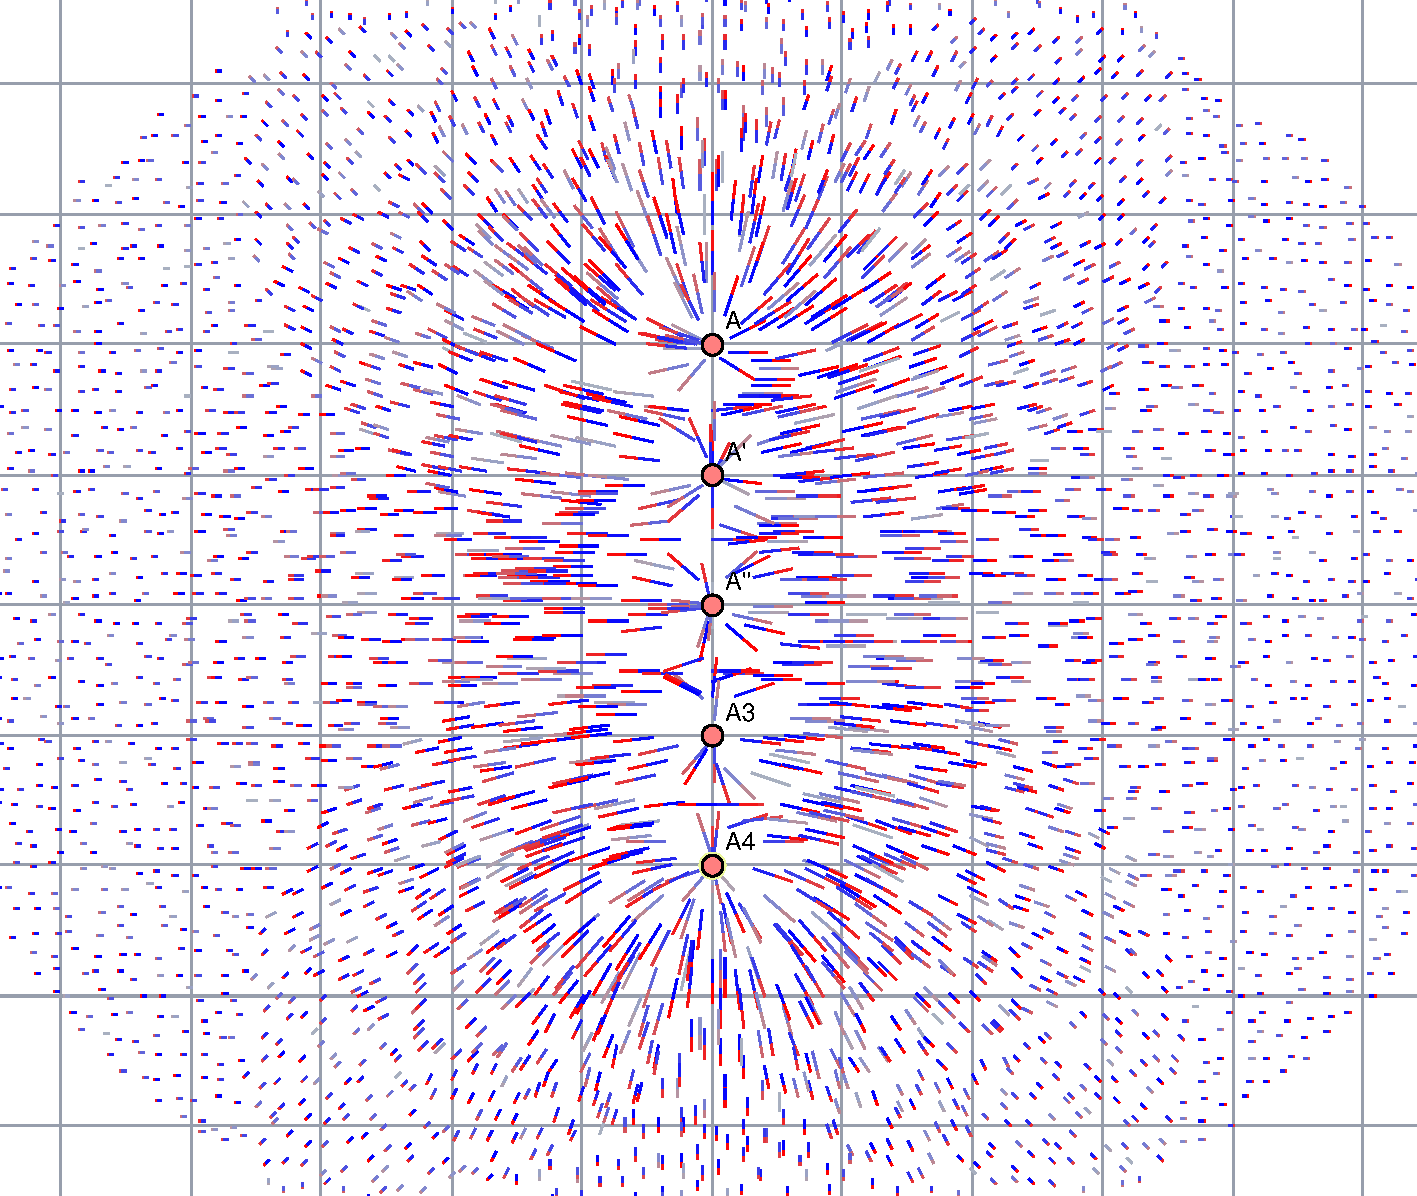
\includegraphics[width=0.7\textwidth]{bilder/efeld_platte}
   \caption{E-Feld einer Platte}
   \label{abb_E-feld-Platte}
\end{figure}


Wir integrieren nun "uber ein kastenf"ormiges Volumen $V$, welches
parallel der Platten die Fl"ache $A_0$ hat und welches im homogenen
Bereich des E-Felds liegt, und einen Teil der Platte zwischen sich
einschlie"st.

Die $\diff \vec A$ aus Gl. \eqref{eqn_gauss-handwerk} stehen senkrecht
auf den Kastenoberfl"achen und sind somit nur auf den Seiten parallel
zur geladenen Platte (die mit Fl"ache $A_0$) parallel zu $\vec E$ -- an
den vier anderen Seitenfl"achen ist $\diff \vec A \bot \vec E$ und
damit $\vec E \cdot \diff \vec A = \langle \vec E | \diff \vec A
\rangle = 0$. An den Fl"achen parallel der Platte ist $\vec E \cdot
\diff \vec A = \langle \vec E | \diff \vec A \rangle = E \cdot A$. Es
muss also gelten:\footnote{Die 2 kommt daher, dass man vorne und
  hinten jeweils eine Fl"ache $A_0$ hat.}
\begin{equation}
   \label{eq:196}
\Phi_E^{(\text{Platte})} =    \int_{\partial V} \vec E \cdot \diff \vec A = 2 \cdot A_0 \cdot E
   \stackrel{\text{\textsc{Gauss}}}{\equiv} \frac{Q}{\varepsilon_0}
\end{equation}
oder umgeformt:\index{E-Feld!Platte}
\begin{equation}
   \label{eqn_e_platte}
   E = \frac{1}{2\varepsilon_0} \cdot \frac{Q}{A} =:
\boxed{   \frac{\sigma}{2\varepsilon_0} = E_\text{Platte}}
\end{equation}
Dabei definieren wir:
\begin{Def}
   [\index{Fl"achenladungsdichte}Fl"achenladungsdichte $\sigma$]
Die Fl"achenladungsdichte $\sigma$ ist Quotient aus Ladung $Q$ und
Fl"ache $A$, auf die $Q$ verteilt ist:
\begin{equation}
   \label{eqn_differenz-c00}
   \sigma = \frac{Q}{A}
\end{equation}
\end{Def}
mit der Einheit $[\sigma] =
\frac{\operatorname{C}}{\operatorname{m^2}}$.

Man sagt auch, $\sigma$ ist "`\textit{Ladung pro Fl"ache}"'.

\begin{Wichtig}
\label{wichtig_unendl-platte}
   $E$ ist bei der unendlich gro"sen Platte unabh"angig vom Abstand zur Platte.
\end{Wichtig}





\subsubsection{Plattenkondensator}
\label{kap_plattenkondensator}

Wir betrachten zwei unendlich ausgedehnte, parallele Platten, die
gegenpolig aber gleich stark geladen sind. Nach dem
Superpositionsprinzip hebt sich das E-Feld aus Symmetriegr"unden
au"serhalb des Kondensators weg (wir verwenden dazu Wichtig
\ref{wichtig_unendl-platte}: Das E-Feld der beiden Platten ist von der
Entfernund unabh"angig) und verst"arkt sich in seinem Inneren noch.

\begin{figure}[h]
   \centering
   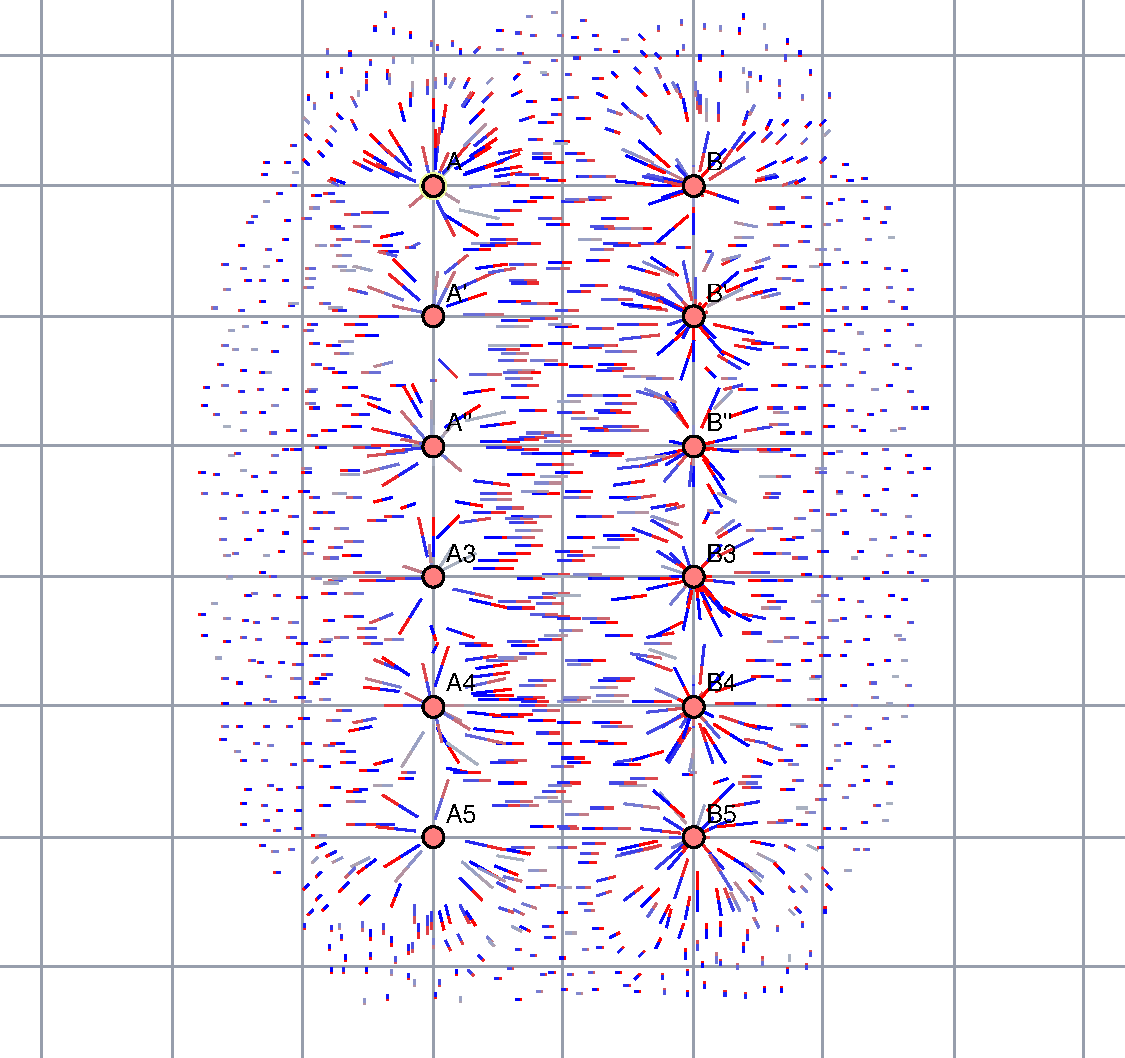
\includegraphics[width=0.7\textwidth]{bilder/efeld_kondensator}
   \caption[E-Feld im Plattenkondensator]{(reales) E-Feld eines
     Plattenkondensators; f"ur uns ist dieses Feld \emph{im}
     Kondensator (also zwischen den Platten) in guter N"aherung
     homogen und verschwindet au"serhalb.}
   \label{abb_efeld-plattenkondensator}
\end{figure}
Im Inneren liegen also doppelt so viele Feldlinien vor, als bei einer
einzelnen Platte, weil die Feldlinien von beiden Platten sich
konstuktiv "uberlagern, weil beide Felder in die gleiche Richtung
zeigen (weg von der positiv geladenen Platte):
\begin{equation}
   \label{eq:199}
   \Phi_E^{(\text{Kondensator})} = 2 \cdot \Phi_E^{(\text{Platte})}
\end{equation}
Damit gilt also:\index{E-Feld!Kondensator}
\begin{equation}
   \label{eqn_differenz-c01}
   \boxed{
E_\text{Kondensator} = \frac{\sigma}{\varepsilon_0}
}
\end{equation}


\abs
Mit \eqref{eq:184} und weil zwischen den Platten das Feld homogen ist
(und sich dadurch eine Probeladung senkrecht zu den Platten bewegen
w"urde, also parallel zu $\vec E$ und damit $\langle \vec E | \diff
\vec s  \rangle = E \cdot s$) gilt weiter (mit $s = d$ als Plattenabstand):
\begin{equation}
   \label{eqn_differenz-c02}
   U = E \cdot d = \frac{\sigma}{\varepsilon_0} \cdot d ~ ~
   \Rightarrow ~ ~
U \sim Q
\end{equation}

F"ur die Proportionalit"at definieren wir:
\begin{Def}
   [\index{Kapazit"at}Kapazit"at $C$]
Das "`\emph{Fassungsverm"ogen} f"ur elektrische Ladungen"' ist
\begin{equation}
   \label{eqn_differenz-c04}
   C = \frac{Q}{U}
\end{equation}
\end{Def}
mit der Einheit $[C] = \frac{\operatorname{C}}{\operatorname{V}} =
\operatorname{F}$ (Farad).

\bigskip
F"ur $C$ gilt beim Plattenkondensator:
\begin{equation}
   \label{eqn_differenz-c05}
   C_\text{Plattenkondensator} = \frac{\varepsilon_0 \cdot A}{d}
\end{equation}




\subsubsection{Exkurs: Schaltung von Plattenkondensatoren}
\label{kap_schaltung-von-plattenkondensatoren}

Wir k"onnen zwei \textbf{parallel} geschaltete \index{Parallelschaltung
  von Kondensatoren}Kondensatoren $C_1$ und $C_2$ als einen gro"sen
interpretieren; die Ladungen den einzelnen Kondensatoren addieren
sich:
$$
Q = Q_1 + Q_2
$$
und die Spannung bleibt gleich. Also gilt mit \eqref{eqn_differenz-c04}
\begin{equation}
   \label{eqn_differenz-c06}
   C = \frac{Q_1 +  Q_2}{U} = \frac{Q_1}{U} + \frac{Q_2}{U} = \boxed{ C_1 +
   C_2 =   C_\text{parallel}}
\end{equation}



Bei zwei \textbf{in Reihe} geschalteten ("`seriellen"') Kondensatoren
ist die Ladung auf den "`inneren"' Platten gleich mit verschiedenen
Vorzeichen, also verschwindet die Summe der Ladung auf den Inneren
Platten und die "au"seren Platten tragen so effektiv die Ladung $Q = Q_1
= Q_2$.

Dagegen Teilt sich die Spannung $U$ in zwei Teile auf:
$$
U = U_1 + U_2
$$
Und so gilt wieder nach \eqref{eqn_differenz-c04}:
\begin{equation}
   \label{eqn_differenz-c07}
   C = \frac{Q}{U_1 + U_2} =
%  \left ( \frac{Q}{U_1 + U_2}  \right
%    )^{(-1) \cdot (-1)} =
\left ( \frac{U_1 + U_2}{Q} \right )^{-1} =
\boxed{
\left ( C_1^{-1} + C_2^{-1} \right )^{-1} = C_\text{reihe}
}
\end{equation}






\subsubsection{sehr langer, geladener Draht}
\label{kap_unendlich-langer-geladener-draht}


Wir definieren die
\begin{Def}
   [\index{Lineare Ladungsdichte}Lineare Ladungsdichte $\lambda$] Als
   Quotient "`Ladung pro L"ange"' eines mit $Q$ geladenen Leiters der
   L"ange $L$
\begin{equation}
   \label{eqn_differenz-c09}
   \lambda = \frac{Q}{L}
\end{equation}
\end{Def}
mit der Einheit $[\lambda] =
\frac{\operatorname{C}}{\operatorname{m}}$.

Nach dem Superpositionsprinzip stellen wir uns das E-Feld dieses
Leiters also radialsymmetrisch zum Leiter vor: Die E-Feldlinien stehen
stets senkrecht auf der Oberfl"ache, da der Leiter praktisch unendlich
ausgedehnt (sehr lang!) ist; nur an den Endpunkten erwarten wir wieder
das ver"anderte Feld einer Punktladung.

Wir integrieren nun "uber ein Zylinderf"ormiges Volumen der L"ange $L$
und mit Durchmesser $2r$ (gr"o"ser als Leiter), welches den Leiter
symmetrisch umschlie"st. Die Fl"achennormale $\diff \vec A$ zeigt hier
stets Parallel zu $\vec E$ und damit ist wieder $\langle \vec E |\diff
\vec A \rangle = E \cdot \diff A$. Die Fl"ache $A$ ist also $2\pi r L$.

An den Zylinderenden ist $\vec E \bot \diff \vec A$ und verschwindet
hier das Skalarprodukt. Wir erhalten also nach
\eqref{eqn_gauss-handwerk}:
\begin{equation}
   \label{eqn_differenz-c10}
   \Phi_E^{(\text{Draht})} = \int_{\partial V} \vec E \diff \vec A = E \cdot 2\pi
   r L \stackrel{\text{\textsc{Gauss}}}{=} \frac{Q}{\varepsilon_0} = \frac{\lambda \cdot L}{\varepsilon_0}
\end{equation}
und damit:\index{E-Feld!Draht}
\begin{equation}
   \label{eqn_differenz-c11}
   \boxed{E_\text{Draht} = \frac{\lambda}{2 \pi r \cdot
       \varepsilon_0}} 
% =
%    \frac{Q}{2\pi r \, L \cdot \varepsilon_0} =
%    \boxed{\frac{\sigma}{\varepsilon_0} = E_\text{Draht}}
\end{equation}








\subsubsection{Koaxialkabel}
\label{kap_koaxialkabel}

Ein Leiter (Au"sendurchmesser $2R_1$) wird durch eine leitende
"`H"ulle"' umschlossen (Innendurchmesser $2R_2$). Zwischen ihnen ist
Platz. Die Ladungsmenge im inneren Leiter ist von der Menge her gleich
und im Vorzeichen verschieden zur Ladung auf der H"ulle.

Wir umschlie"sen den Leiter wieder mit einem zylinderf"ormigen Volumen
der L"ange $L$ und dem Durchmesser $2r$.

Die E-Feldlinien gehen wieder senkrecht durch die Zylinderwand und es
gilt damit $\langle \vec E |\diff \vec A  \rangle = E \cdot \diff A$,
wobei $A = 2\pi r \cdot L$ und damit f"ur konstantes $L$:
$
\diff A = \diff (2\pi r L) = 2 \pi L \diff r
$

Es gilt also (mit konstantem $\lambda$):
\begin{equation}
   \label{eqn_differenz-c12}
   \Phi_E^{(\text{Koax})}
=
\int_{\partial V} \vec E \diff \vec A
=
E \cdot 2 \pi L \cdot  r
\stackrel{\text{\textsc{Gauss}}}{=}
\frac{Q}{\varepsilon_0} = \frac{\lambda \cdot L}{\varepsilon_0}
\end{equation}
und damit:\index{E-Feld!Koaxkabel}
\begin{equation}
   \label{eqn_differenz-c13}
  \boxed{ E(r) = \frac{\lambda}{2 \pi \cdot \varepsilon_0 \cdot r}} ~ ~ ~
   \text{ mit } R_1 \leq r \leq R_2
\end{equation}
Wenn $r < R_1$, so ist $E = 0$, weil die Ladungen sich auf der
Au"senseite des Leiters verteilen. Nach dem Satz von Gauss
verschwindet also die eingeschlossene Ladung und damit auch das
E-Feld. F"ur $r > R_2$ ist es ebenso: Die Summe der Ladungen im
eingeschlossenen Volumen verschwindet und damit auch das E-Feld.

F"ur den Raum dawischen existiert aber offensichtlich ein E-Feld,
welches nach au"sen hin abnimmt.

Wir k"onnen die Spannung f"ur den Abstand $r$ vom inneren Leiter nach
Gl. \eqref{eq:184} bekommen:\footnote{Wir setzen hier wieder $\langle
  \vec E | \diff \vec s \rangle = E \cdot \diff s$, weil wir den
  k"urzesten Weg zwischen zwei Untersuchten Punkten w"ahlen: Die
  direkte, radiale Verbindung, parallel zu $\vec E$.}
\begin{equation}
   \label{eqn_differenz-c14}
   U(r) = \int_{R_1}^r \vec E \diff \vec s =
\int_{R_1}^r E \diff s  =
\int_{R_1}^r \frac{\lambda}{2 \pi \cdot \varepsilon_0 \cdot r} \diff r
=
\frac{\lambda}{2 \pi \cdot \varepsilon_0} \cdot \ln \frac{r}{R_1}
\end{equation}
und mit \eqref{eqn_differenz-c04}:
\begin{equation}
   \label{eqn_differenz-c15}
   C = \frac{Q}{U(R_2)}
   =
   \frac{ \lambda L \cdot 2\pi \cdot \varepsilon_0}{\lambda \cdot \ln
     \frac{r}{R_1}}
=
   \frac{L \, 2\pi  \cdot \varepsilon_0}{\ln
     \frac{r}{R_1}}
\end{equation}


\begin{figure}
   \centering
   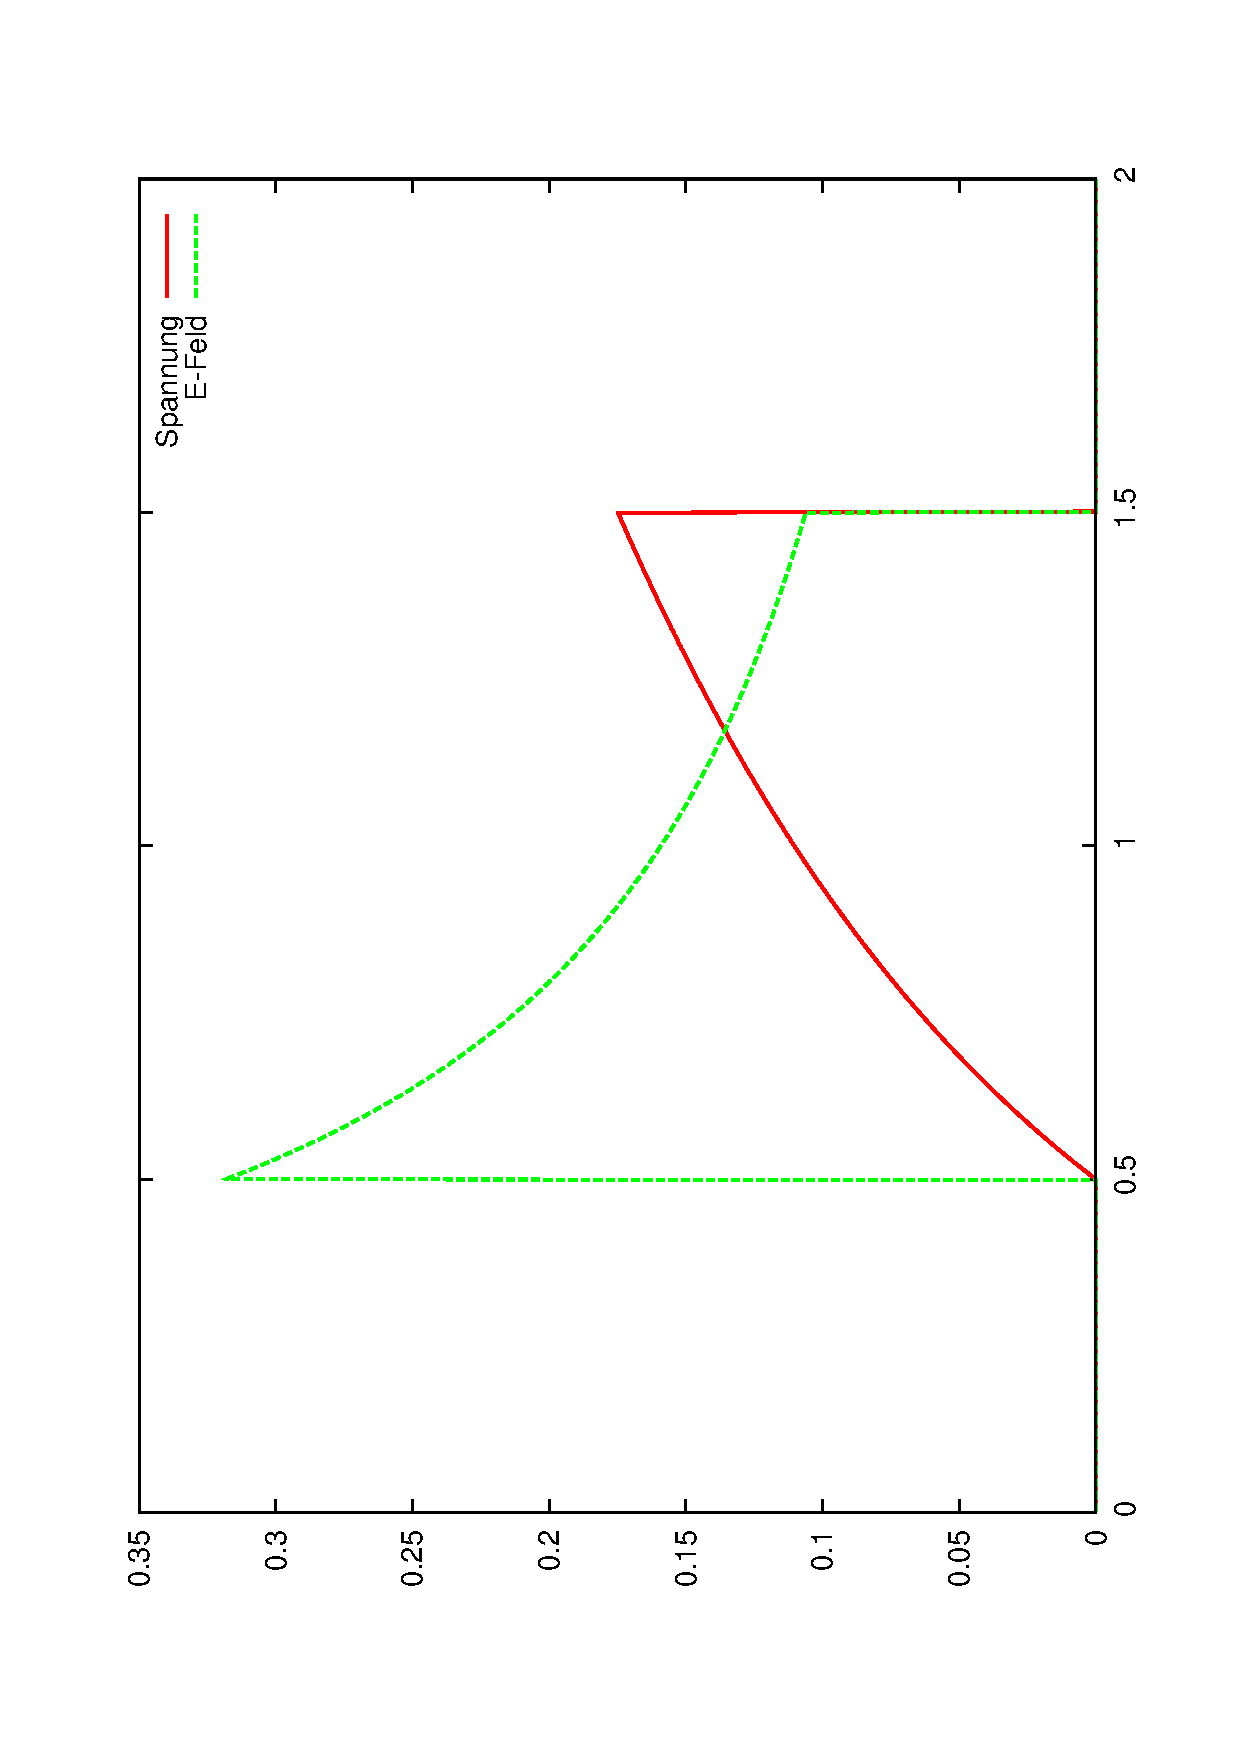
\includegraphics[width=0.5\textwidth,angle=-90]{bilder/koax}
   \caption[Spannung und E-Feld im Koaxkabel]{Spannung und E-Feld im
     Koaxkabel; der Au"sendurchmesser des Leiters ist 1, der
     innendurchmesser der H"ulle ist 3 (und hier ist der \emph{Radius}
     auf der $x$-Achse). Siehe
     Gl. \eqref{eqn_differenz-c13} und \eqref{eqn_differenz-c14}}
   \label{abb_koax}
\end{figure}






\subsubsection{Homogen geladene, nicht leitende Kugel}
\label{kap_homogen-geladene-nicht-leitende-kugel}


% Innerhalb einer Hohlkugel mit Radius $R_2$ ist eine geladene Kugel
% zentrisch mit Radius $R_1$. Die Beide Kugeln sind betragsm"a"sig gleich
% aber gegenpolig geladen und die Kugeln sind nicht leitend, die
% Ladungen aber homogen verteilt.
Auf einer Kugel mit Radius $R$ ist die Ladung $Q$ homogen verteilt
und die Kugel ist nicht leitend.
\begin{Def}
   [\index{nicht leitend}nicht leitend] bedeutet dabei, dass die
   Ladungen fixiert sind.
\end{Def}

Wir integrieren "uber eine zentrische Kugel mit Radius $r$ und
Oberfl"ache $A = 4 \pi r^2$. Die E-Feldlinien zeigen wieder
senkrecht zur Fl"ache $A$, also $\langle \vec E | \diff \vec A  \rangle
= E \cdot \diff A = E \cdot 8 \pi \cdot r \diff r$. Es gilt
also:
\begin{equation}
   \label{eqn_differenz-c16}
   \Phi_E^{(\text{Kugel})} = \int_{\partial V} \vec E \diff \vec A
=
\int_{0}^r E \cdot 8 \pi \cdot \hat r \diff \hat r
=
4 \pi  \cdot E \cdot r^2 \stackrel{\text{\textsc{Gauss}}}{=} \frac{Q}{\varepsilon_0}
\end{equation}
und damit\index{E-Feld!Kugel}
\begin{equation}
   \label{eqn_differenz-c03}
   \boxed{
E_\text{Kugel}(r) = \frac{Q}{4 \pi \cdot \varepsilon_0 \cdot r^2}
 }  ~ ~ ~  \text{ mit } r \geq R
\end{equation}

Weil hier die Ladungen fixiert sind, gilt im inneren der Kugel ein
anderer Zusammenhang; hier ist die Ladung $Q$ homogen verteilt, und damit
ist
$$
\varrho = \frac{Q}{\frac{4}{3} \pi R^3}
$$
und damit die Ladung innerhalb der Kugel mit Radius $r$ (mit $r \leq
R$):
$$
\tilde Q = \varrho \cdot \tilde V = \varrho \cdot \frac{4}{3} \pi r^3
$$
Es gilt also nach Gl. \eqref{eqn_differenz-c16}:
\begin{equation}
   \label{eqn_differenz-c08}
     \Phi_E^{(\text{Kugel, innen})} =
4 \pi  \cdot E \cdot r^2 \stackrel{\text{\textsc{Gauss}}}{=} \frac{\varrho \cdot \frac{4}{3} \pi r^3}{\varepsilon_0}
\end{equation}
und damit
\begin{equation}
   \label{eqn_differenz-c17}
\boxed{   E_\text{Kugel, innen}(r) = \frac{Q \cdot
   r}{4\pi \cdot \varepsilon_0 \cdot R^3} }
~ ~ ~ \text{ mit } r \leq R
\end{equation}


\bigskip
Analog zu Kap. \ref{kap_koaxialkabel} berechnen wir noch die Spannung au"sen:
\begin{equation}
   \label{eqn_differenz-c18}
   U_a(r) = \int_R^r \vec E \diff \vec s = \int_R^r E \diff s
=
\int_R^r \frac{Q}{4 \pi \cdot \varepsilon_0 \cdot \hat r^2} \diff \hat
r = \left [\frac{-Q}{4\pi \varepsilon_0 \hat r} \right ]_R^r
\end{equation}
% und innen:
% \begin{equation}
%    \label{eqn_differenz-c20}
%    U_i(r) = \int_0^r E \diff s = \frac{-Q \cdot r^2}{8\pi \cdot \varepsilon_0 \cdot R^3}
% \end{equation}
% Das "`$-$"' kommt daher, dass im Inneren der Kugel das E-Feld in die
% andere Richtung l"auft.

Wenn wir die Kapazit"at bestimmen wollen, so denken wir uns die zweite
Platte in der Unendlichkeit. Mit \eqref{eqn_differenz-c04} gilt:
\begin{equation}
   \label{eqn_differenz-c19}
   C = \frac{Q}{U_a(\infty)} = 4 \pi \varepsilon_0 \cdot R
\end{equation}

\begin{figure}
   \centering
   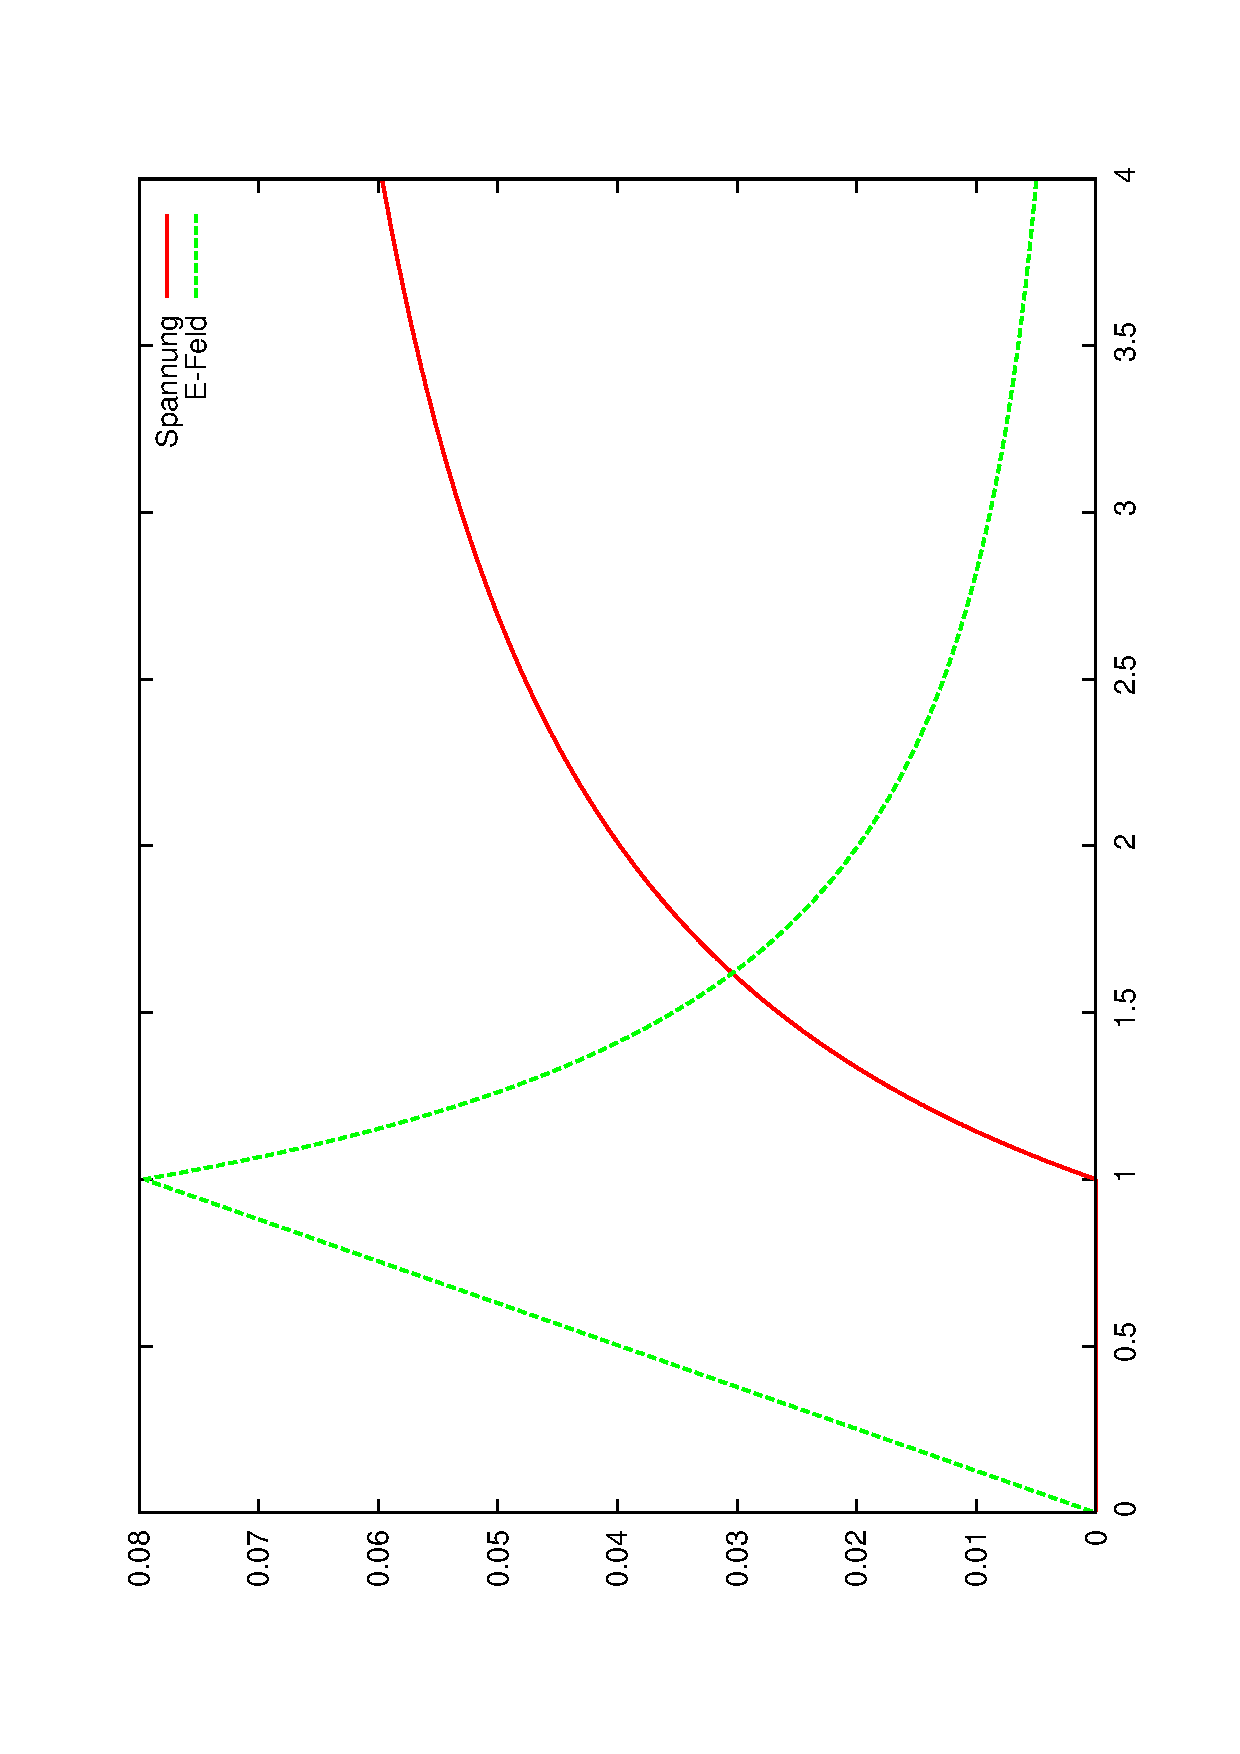
\includegraphics[width=0.5\textwidth,angle=-90]{bilder/kugel}
   \caption[E-Feld einer Kugel]{E-Feld um eine geladene Kugel mit
     fixierten Ladungen. $R = 1$}
   \label{abb_efeld_kugel}
\end{figure}



\begin{Wichtig}
   F"ur die Kapazit"at einer einzelnen Ladung interpretiert man diese
   als Teil eines Kondensators mit $d = \infty$.
\end{Wichtig}





\subsection{Vergleich der E-Felder}
\label{kap_vergleich-e-felder}

Die berechneten E-Felder kann man nun schnell vergleichen; siehe
Tab. \ref{tab_glg_e-feld_symmetrie}.

\begin{table}[h]
   \centering
   \begin{tabular}{l c c c}
      \toprule
      Form: & \textbf{Kugel} & \textbf{Draht} & \textbf{Platte}\\
      \midrule
      $E = $ &
      $\frac{Q}{4\pi r^2 \varepsilon_0} $  &
      $ \frac{Q}{2\pi r L \varepsilon_0}$ &
      $\frac{Q}{2A \varepsilon_0}$
    \\
      Abh. von $\frac{R}{r}$ &  $\frac{Q}{A \varepsilon_0}\left ( \frac{R}{r} \right )^2$&
      $\frac{2Q}{A \varepsilon_0} \left ( \frac{R}{r} \right )^1$&
      $\frac{Q}{2A \varepsilon_0}$
    \\
      Ausbreitung von $E$: & 3 Dim. & 2 Dim. & 1 Dim\\
      \bottomrule
\end{tabular}
   \caption{Vergleich der E-Felder bei verschiedenen Symmetrien}
   \label{tab_glg_e-feld_symmetrie}
\end{table}






\subsection{E-Feld im Leiter}
\label{kap_e-feld-im-leiter}

\begin{Def}
   [\index{Leiter}Leiter] Material, in welchem sich Ladungstr"ager
   m"oglichst leicht bewegen k"onnen.
\end{Def}
Das klassische Beispiel sind Metalle, hier sind die Elektronen als
"`\index{Elektronengas}Elektronengas"' frei und von den R"umpfen
unabh"angig beweglich.

Da die Elektronen frei beweglich sind, wirkt auf sie insgesamt keine
Kraft ($F = 0$)  und wegen \eqref{eqn_e-feld} darf auch kein E-Feld
existieren: $E = 0$:
\begin{Wichtig}
   Innerhalb eines Leiters herrscht kein E-Feld.
\end{Wichtig}

Aus dem Satz von \textsc{Gauss} (Kap. \ref{kap_satz-von-gauss}) folgt
nun, dass wenn das E-Feld verschwindet, in einem eingeschlossenen
Volumen keine Quellen -- also Ladungen -- vorhanden sein d"urfen:
Betrachten wir das komplette (innere) Volumen des Leiters, so muss
hier folglich $\varrho = 0$ sein. Die Ladungen halten sich also nicht
im Inneren des Leiters auf; damit m"ussen sie sich (um "uberhaupt im
Leiter zu sein) auf einer schmalen "au"seren Fl"ache befinden; hier haben
die Ladungen au"serdem dem maximalen Abstand voneinander.

Da die Ladungen auf der Schicht au"sen \emph{bleiben}, m"ussen sie auf
einer "Aquipotentialfl"ache liegen und damit muss das E-Feld
\emph{senkrecht} zur Leiteroberfl"ache liegen (weil
"Aquipotentialfl"achen immer senkrecht zu den Feldlinien liegen).

\begin{Beispiel}
Wir betrachten nun ein Leiterende -- als Kugel ausgef"uhrt. Hier gilt
mit \eqref{eq:177} und \eqref{eqn_differenz-c03} direkt am Leiterende:
$$
E_\bot = \frac{Q}{4\pi R^2\, \varepsilon_0} \text{ und } U =
\frac{Q}{4\pi R\, \varepsilon_0}
$$
und damit
$$
E_\bot = \frac{U}{R}
$$
D.h. $E_\bot$ ist proportional zu $U$ und reziprok %\emph{quadratisch}
proportional zu $R$. F"ur kleien $R$ wird also $E$ \emph{sehr} gro"s.

Wenn man also einen Leiter mit einer Spitze oder einer scharfen Kante
o."a. hat, so wird an dieser Stelle das E-Feld extrem gro"s werden. Es
kann sogar dazu kommen, dass Elektronen und Atome ausgeschleudert
werden. Man wendet dies bspw. bei der
\emph{\index{Feldlinienemmission}Feldlinienemmission} an: Dabei gibt
man auf eine Metallspitze eine hohe Spannung: Hier wird $E$ sehr gro"s
und es werden Elektronen ausgeschleudert, die man als Elektornenstrahl
verwenden kann.
\end{Beispiel}

% \begin{equation}
%    \label{eqn_differenz-c21}
% \int_A   E_\bot \diff A = E_\bot 4\pi R^2 = \frac{Q}{\varepsilon_0}
% \text{ und damit } E_\bot(r) = \frac{Q}{4\pi R^2 \cdot \varepsilon_0}
% \end{equation}
% Und mit \eqref{eq:184}:
% \begin{equation}
%    \label{eqn_differenz-c22}
%    U(r) =  \frac{Q}{}
% \end{equation}

% In n"achste N"ahe des Drahtes sind die Feldlinien praktisch parallel und
% wir behandeln diese Stelle als Plattenkondensator und erhalten (in
% 1. N"aherung):
% \begin{equation}
%    \label{eqn_differenz-c23}
%    E = \frac{U}{r}
% \end{equation}
% Die Spannung $U$ h"angt davon ab, welcher Strom im Leiter flie"st: Je
% mehr Strom, desto mehr Ladung, die ein st"arkeres E-Feld aufbaut und so
% eine gr"o"sere Potentialdifferenz "`bereitstellt"'.






\subsection{\textsc{Faraday}scher K"afig}
\label{kap_faradayscher-kafig}

Wir betrachten einen abgeschlossenen Hohlraum in einem Metall oder
einem anderen Leiter:
\begin{Wichtig}
   In metallischen Hohlr"aumen herrscht kein E-Feld: $E = 0$.
\end{Wichtig}

Wenn dem \emph{nicht} wo w"are, h"atten wir ein E-Feld, welches von
Ladungen erzeugt wird. Nun w"urden aber die Ladungen im Hohlraum (also
in der Luft) dem E-Feld folgen und auf das Metall gebracht
werden.

Damit w"urde das potentielle E-Feld nur durch Ladungen im Metall
aufgespannt. Diese Ladungen w"urden aber selbst dem E-Feld folgen (das
E-Feld sorgt f"ur ein Potentialgef"alle, dem die Ladungen folgen wollen)
also einfach "`abflie"sen"' anstatt ein E-Feld aufzubauen.

\begin{Beispiel}
Der
\textbf{\textsc{\index{Van-De-Graaf-Generator}Van-De-Graaf}}-Generator
funktioniert nach diesem Prinzip: Ladung wird auf ein "`F"orderband"'
augenommen und damit auf das Innere einer Metallkugel gegeben. Das ist
ohne Arbeitsaufwand m"oglich, weil in der Kugel ja kein E-Feld herrscht
und die Elektronen so keine Gegenkraft erfahren. Einmal auf die Kugel
gebracht, bewegen sich die Ladungen nach au"sen, weil sie hier den
gr"o"sten Abstand voneinander haben k"onnen. Auf der Kugelau"senseite
k"onnen sich so sehr hohe Spannungen bilden.
\end{Beispiel}






\subsection{Influenz}
\label{kap_influenz}

Bringt man einen Leiter in ein E-Feld, so erfahren die Ladungen im
Leiter eine elektrische Kraft und werden (da im Leiter beweglich)
abgelenkt. Sie bilden so eine Zone mit Mangel und eine mit "Uberfluss
und dazwischen ein E-Feld
("`\textbf{\index{Gegenfeld}Gegenfeld}"').

\begin{Def}
[\index{Influenzladungen}Influenzladungen]  Quellen des Gegenfelds.
\end{Def}

Die Ladungen werden sich so
lange bewegen, bis das neue, innere E-Feld so stark ist, wie das
"au"sere: Wenn dem so ist, heben die Felder sich duch Superposition im
Inneren des Leiteres gegenseitig weg und die Ladungen haben keinen
Grund (keine elektrische Kraft) mehr, sich zu bewegen.

Au"serdem werden die bewegten Ladungen durch Reibung gebremst und wenn
die Reibungskraft nicht permanent von einer elektrischen Kraft
"uberwunden wird, wird die Ladung immer langsamer und bleibt
schlie"slich stehen.

Im Unterschied dazu haben \textbf{\index{Supraleiter}Supraleiter}
keinen Widerstand. Die Ladungen werden also, wenn keine Kr"afte durch
E-Felder auf sie wirken, nicht abgebremst. In Supraleitern bleibt also
die Bewegung der Ladungen gleich: Man kann endlose Str"ome erzeugen.




\subsection{Prinzip der Bildladungen}
\label{kap_prinzip-bildladungen}

\begin{Wichtig}
   In einem Leiter verteilen sich die Ladungen so, dass der Rand des
   Leiters eine "Aquipotentialfl"ache ist.
\end{Wichtig}
Wenn dem nicht so w"are, w"urden sich die Ladungen so verschieben, dass
dem so ist: Mit dem selben Argument wie in Kap
\ref{kap_faradayscher-kafig} m"ussen sich alle Ladungen auf dem Rand
verteilen. Wenn nun eine Stelle am Rand weniger dicht und eine andere
dichter, so w"urden die Ladungen zur Stelle niedrigerer Dichte flie"sen,
weil sie nach dieser Stelle angezogen werden. Ebenfalls analog zu
\ref{kap_e-feld-im-leiter} muss das E-Feld nun senkrecht auf der
Oberfl"ache des Leiters stehen.

Das Problem ist nun, das E-Feld zu \emph{bestimmen}, welches au"serhalb
des Leiters existiert: Weil die Feldlinien immer senkrecht auf der
Oberfl"ache stehen m"ussen und die Geometrie der Oberfl"ache beliebig
kompliziert sein kann, kann das E-Feld ziemlich komplizierte Formen
annehmen; Wir f"uhren deswegen die \emph{Bildladungen} ein:
\begin{Def}
   [\index{Bildladung}Bildladung] Eine Bildladung $q'$ ist eine
   gedachte Ladung in einem Leiter, die auf eine Ladung $q$ au"serhalb
   des Leiters so wechselwirkt, wie es der Leiter tut.

   Eine Bildladung $q'$ ist betragsm"a"sig gleich $q$ mit
   verschiedenen Vorzeichen ($q =-q'$).
\end{Def}
Wir ersetzen also die Wechselwirkung des Leiters durch die
Wechselwirkung mit einer anderen Ladung.

Die Idee dahinter: Wir betrachten zwei Ladungen $Q^+$ und $Q^-$ mit
ihrem Coulomb-Feld und schieben eine d"unne Metallplatte genau zwischen
die beiden Ladungen. Die Platte nimmt Influenzladungen $q$ an, sodass
das "au"sere E-Feld im Prinzip nicht gest"ort wird: Jetzt laufen die
E-Feldlinien nicht mehr von Ladung $Q^-$ zu $Q^+$ sondern von $Q^+$ zu
$q^-$, haben aber die selbe Form und St"arke wie vorher.

Entfernt man nun eine der beiden Ladungen und ersetzt sie durch einen
kompakten Leiter, so hat man das "au"sere E-Feld immer noch nicht
gest"ort; es besteht jetzt zwischen einer Ladung (oBdA) $Q^+$ und den
Influenzladungen $q^-$.

Die Influenzladungen aus unserer Idee sind nun die
\emph{tats"achlichen} Ladungen auf der Oberfl"ache eines Leiters -- und
diese k"onnen wir jetzt genau durch die Ladung $Q^-$ ersetzen.

Damit m"ussen wir auch $\varrho(\vec r)$ nicht genauer ausrechnen und
verwenden stattdessen das "uberlagerte Feld der Bildladungen.


\begin{figure}
   \centering
   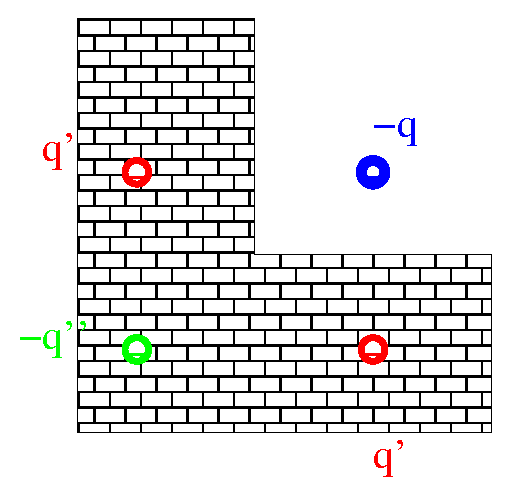
\includegraphics[width=0.6\textwidth]{bilder/bildladung}
   \caption[Bildladungen]{Prinzip der Bildladungen: 1. Generation in
     Blau, 2. in Rot und 3. in Gr"un}
   \label{abb_bildladungen}
\end{figure}





\begin{Wichtig}
   Spiegeln wir eine Ladung $-q$ au"serhalb eines Leiters an an jeder
   Oberfl"ache (bzw. deren Verl"angerung) des Leiters, erhalten wir
   mehrere $q'$ ("`1. Generation"'). Man muss nun auch diese $q'$ an
   den Oberfl"achen spiegeln ($q'' = -q'$: "`2. Generation"'), bis
   jede weitere Spiegelung eine Ladung auf eine andere spiegeln
   w"urde.
\end{Wichtig}





\subsection{Energie des E-Felds}
\label{kap_energie-des-e-felds}

M"ochte man einen Kondensator aufladen, so braucht man daf"ur Energie:
Die bereits auf den Platten vorhandenen Ladungen sto"sen die neu
dazukommenden Ladungen ab und diese Absto"sungen gilt es zu
"uberwinden.

Um die Kraft, mit der abgesto"sen wird, zu bestimmen, stellt man
folgende "Uberlegung an: Um eine Platte positiv zu laden, muss man
hier alle negativen Ladungstr"ager der Ladung $q = q^-$ -- alle Elektronen
-- abziehen und auf die negative Platte bringen. Dazu muss man also
das einzelne Elektron mit den E-Feldlinien bewegen -- und somit gegen
die Kraft $\vec F = \vec E \cdot q^-$, und daf"ur braucht man die
Arbeit $W_q = \int_\gamma \vec F \cdot \diff \vec s$. Ob man nun die
Elektronen wirklich innerhalb des Kondensators direkt gegen das E-Feld
bewegt oder nicht, ist nicht entscheidend, weil das E-Feld ja
wirbelfrei ist (vgl. Kap. \ref{kap_elektrisches-potential}).

F"ur einen (Platten)Kondensator der Breite $a$ gilt wegen $E =
\frac{U}{a}$ (vgl. \eqref{eqn_differenz-c02}) also:
\begin{equation*}
   \label{eqn_differenz-c24}
   W_q = \int_0^a \frac{U}{a}q \diff s = \frac{U}{a}q \cdot a = U
   \cdot q
\end{equation*}
"Ubertr"agt man nun nicht nur ein einzelnes Elektron, sondern die
Ladung $Q = \int_0^Q 1 \diff q$, so braucht man (mit $U = \frac{q}{C}$
-- vgl. Gl. \eqref{eqn_differenz-c04} -- hier ist $q$ die Ladung, die
sich auf den Platten befindet und von $Q$, der Ladung die St"uck f"ur
St"uck auf die Platten gebracht wird, verschieden) die Arbeit
\begin{equation*}
   \label{eqn_differenz-c25}
   W 
% = \int_0^Q Q\cdot q \diff q 
= \int_0^Q U \cdot \diff q
= \int_0^Q \frac{q}{C} \diff q =
   \frac{1}{2} \frac{Q^2}{C}
\end{equation*}

In unserer Herleitung haben wir allgemeine Annahmen gemacht, die so
nicht nur f"ur den Plattenkondensator gelten, sondern allgemein f"ur
beliebige Kondensatoren: Man kann sich jeden Kondensator vorstellen
als (beliebig komplizierte) Verschaltung von Plattenkondensatoren.

Ersetzt man nun noch nach Gl. \eqref{eqn_differenz-c04} $Q = CU$, erh"alt man:
\begin{Wichtig}
   Die Energie eines beliebigen, mit der Spannung $U$ aufgeladenen
   Kondensators ist
   \begin{equation}
      \label{eqn_energie_kondensator}
      \boxed{  W = \frac{1}{2} C U^2  }
   \end{equation}
\end{Wichtig}

Denken wir uns nun weiter jeden Kondensator aufgebaut aus kleien
Plattenkondensatoren, so k"onnen wir die \textbf{Energiedichte}
bestimmen: Beim Plattenkondensator gilt wegen \eqref{eqn_differenz-c05} und mit
$U = E \cdot a$ (vgl. \eqref{eqn_differenz-c02}):
\begin{equation}
   \label{eqn_differenz-c27}
   W = \frac{\varepsilon_0 A}{a} \cdot \frac{U^2}{2}
=
 \frac{\varepsilon_0 A}{a} \cdot \frac{E^2 \cdot a^2}{2}
=
 \frac{\varepsilon_0 A \cdot E^2 \cdot a}{2}
=
\frac{1}{2} \cdot \varepsilon_0 \cdot E^2 \cdot V
\end{equation}
Und damit:
\begin{Def}
   [\index{r"aumliche Energiedichte}R"aumliche Energiedichte
   $\varrho_{E,V}$  oder $w$]\label{def_energiedichte} Die Energiedichte
    bezeichnet die Verteilung von Energie $W$ auf ein
   Volumen $V$. Bei Kondensatoren gilt:
   \begin{equation}
      \label{eqn_energiedichte_kondensator}
      \boxed{  \varrho_{E,V} = w = \frac{W}{V} = \frac{1}{2} \varepsilon_0
        E^2   }
   \end{equation}
\end{Def}

Eine direkte Folge aus der hier konzentrierten Energie ist eine Kraft
zwischen den Platten des Kondensators; In differenzieller Schreibweise
ist $\diff W = F \diff s$. Wendet man das Differenzial $\diff$ auf
\eqref{eqn_differenz-c27} an, gilt:
\begin{eqnarray*}
   \label{eqn_differenz-c26}
   \diff W &=& \diff \left ( \frac{1}{2} \cdot \varepsilon_0 \cdot E^2
      \cdot V \right )\\
&=& \frac{1}{2} \cdot \varepsilon_0 \cdot E^2 \cdot \diff V\\
&=& \frac{1}{2} \cdot \varepsilon_0 \cdot E^2 \cdot \diff (A \cdot s)\\
&=& \frac{1}{2} \cdot \varepsilon_0 \cdot E^2 \cdot A \cdot \diff s\\
&=& F \cdot \diff s
\end{eqnarray*}
Wobei wir verwenden, dass das E-Feld homogen und damit konstant ist,
ebenso wie die Fl"ache des Kondensators, wobei $s$ der differenzielle
Abstand zu einer Platte ist. Ein Koeffizientenvergleich liefert also
mit \eqref{eqn_differenz-c05} und \eqref{eqn_differenz-c02}:
\begin{equation}
   \label{eqn_differenz-c28}
   F = \frac{1}{2} \cdot \varepsilon_0 \cdot E^2 \cdot A = \frac{1}{2}
   Q E
\end{equation}




\subsection{Isolatoren bzw Dielektrika im E-Feld}
\label{kap_isolatoren-im-e-feld}


\begin{Def}
   [\index{Dielektrikum}Dielektrikum] Ein Dielektrikum ist nichts
   anders als ein Isolator, also ein nicht- oder nur schwach
   stromleitendes Material. Die Ladungstr"ager sind i.A. nicht frei
   beweglich.
\end{Def}

In einem Experiment laden wir einen Kondensator auf und f"uhren
anschlie"send ein Dielektrikum ein. Die Spannung nimmt dabei von $U_0$
auf $U_D$ ab. Man definiert:
\begin{Def}
   [(relative)
   \index{Dielektrizit"atskonstante}Dielektrizit"atskonstante
   $\varepsilon_r$] auch "`relative \index{relative
     Permittivit"at}Permittivit"at"' oder "`Dielektrizit"atszahl"':
   Der Faktor $\varepsilon_r$ gibt an, wie stark sich die Spannung
   (Kapazit"at) beim Einf"uhren des Dielektrikums vermindert
   (erh"oht):
   \begin{equation}
      \label{eqn_def_espilon}
       \varepsilon_r = \frac{U_0}{U_D} =
      \frac{\frac{Q}{U_D}}{\frac{Q}{U_0}} = \frac{C_D}{C_0}
   \end{equation}
\end{Def}
Die Dielektrizit"atszahl ist dimensionslos, also $[\varepsilon_r] = 1$
und h"angt vom Material ab. Siehe dazu
Tab. \ref{tab_dielektrizitaetszahl}.


\begin{table}
   \centering
   \begin{tabular}{l c}
\toprule
      \textbf{Stoff} & \textbf{Dielektrizit"atszahl $\varepsilon_r$}\\
\midrule
Vakuum & 1 ~ ~ \emph{per Definition}\\
Luft & 1.000\, 59\\
Paraffin & 2.1\\
Methanol & 32.6\\
Wasser & 80\\
Eis & 100\\
Spezielle Keramiken & 10\, 000\\
$SrTiO_3$ & 12\, 000\\
\bottomrule
   \end{tabular}
   \caption{Dielektrizit"atszahl ausgew"ahlter Materialien (Quelle:
     \textsc{Bechinger} und \textsc{Wikipedia})}
   \label{tab_dielektrizitaetszahl}
\end{table}



M"ochte man die \textbf{Kapazit"at eines Kondensators} mit Dielektrikum
bestimmen, so gilt, weil die Kapazit"at um $\varepsilon_r$ zunimmt und
weil $C_0 = \varepsilon_0 \cdot \frac{A}{d}$:
\begin{equation}
   \label{eqn_kondensator_dielektrikum}
   C = \varepsilon_r C_0 = \boxed{  \varepsilon_0 \cdot \varepsilon_r \cdot
   \frac{A}{d} = C  }
\end{equation}



\bigskip
\begin{Wichtig}
   Wegen $U \sim E$ nimmt nicht nur die Spannung im Kondensator um
   $\varepsilon_r$ ab, sondern auch die St"arke des E-Felds:
   \begin{equation*}
      E_0 = \varepsilon_r \cdot E_D
   \end{equation*}
\end{Wichtig}

Die \textbf{Ursache} f"ur die Verminderung des E-Felds ist die
{Dielektrische Polarisation}.





\subsection{Die elektrische Polarisation}
\label{kap_dielektrische-polarisation}

Sie ist sehr "ahnlich zur Influenz, nur dass sich hier durch ein
"au"seres E-Feld nur Ladungen \emph{innerhalb} des Molek"uls verschieben
k"onnen.

Legt man an ein Atom oder Molek"ul ein "au"seres E-Feld an (vlg. dazu
Abb. \ref{abb_induz_dipolmoment}), dann wird die Elektronenh"ulle
bez"uglich des Kerns verschoben: Diese Verschiebung geht so lange, bis
die r"ucktreibende Kraft die Kraft, die das angelegte E-Feld auf die
Teilchen aus"ubt ($F = E \cdot q$), kompensiert.

Wenn vorher noch die Schwerpunkte von positiver und negativer Ladung
aufeinanderfielen, so sind diese nun getrennt -- mit dem Abstand
$\delta$. Man f"uhrt einen \emph{Pointing-Vector} $\vec \delta$ ein:
Dieser hat als L"ange besagte Ladungsverschiebung und zeigt vom
Positiven zum Negativen Ladungsschwerpunkt. In seinem Mittelpunkt
liegt der gesamte (neutrale) Ladungsschwerpunkt des Atoms
bzw. Molek"uls.

Gem"a"s Kapitel \ref{kap_elektrisches-potential} und der dortigen
Definition ist das \index{Induzierte Dipolmoment}\textbf{Induzierte
  Dipolmoment}
\begin{equation}
   \label{eqn_differenz-c29}
   \vec p = q \cdot \vec \delta
\end{equation}
wobei $q$ die Ladung des Atoms bzw. Molek"uls ist. (Allgemein ist $q$ der
Betrag der \emph{verschobenen} Ladung, wobei logischerweise ein $q^+$
und ein $q^-$ existieren und $q = |q^+| = |q^-|$.)

\begin{figure}
   \centering
   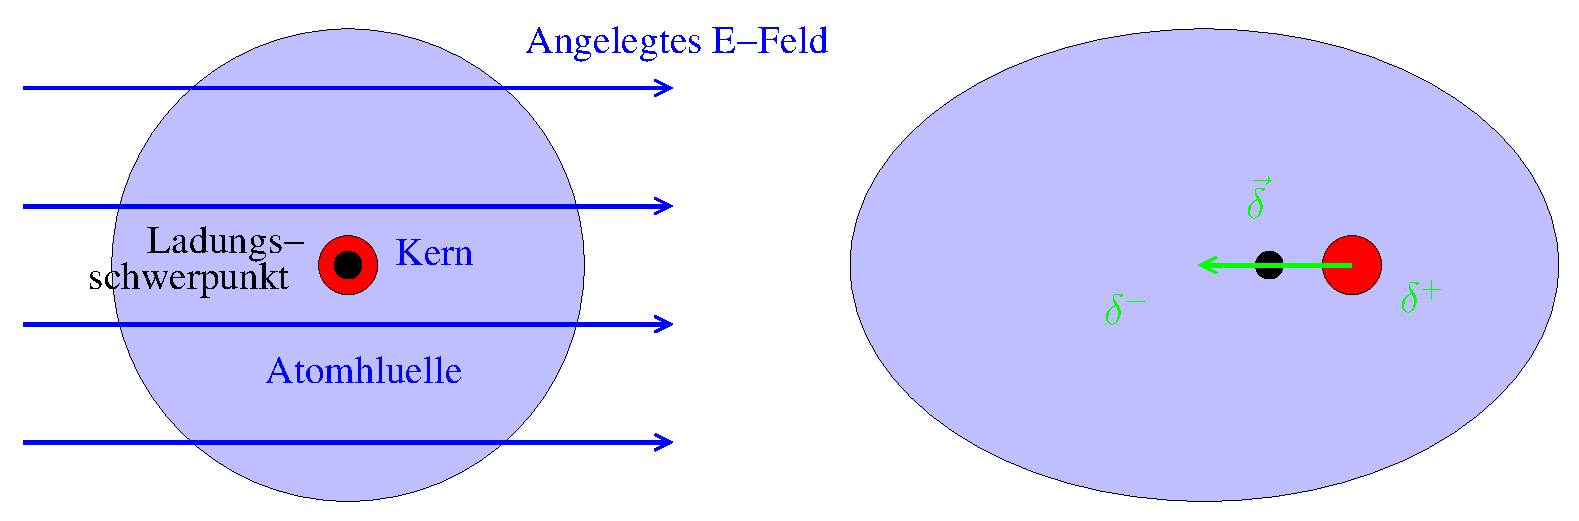
\includegraphics[width=\textwidth]{bilder/induz_dipolmomen}
   \caption[Dipolmoment]{In einem Atom wird durch ein "au"seres E-Feld
     ein Dipolmoment induziert (das linke Bild ist eine Kurzaufnahme
     direkt beim Anlegen des Feldes). Dieses Dipolmoment kompensiert
     das "au"sere E-Feld im Atom. $\vec \delta$ ist ein \emph{pointing
       Vector}\index{pointing Vector} f"ur die Ladungsverschiebung}
   \label{abb_induz_dipolmoment}
\end{figure}


Wir definieren nun:
\begin{Def}
   [\index{Polarisierbarkeit}Polarisierbarkeit $\alpha$] Sie ist ein
   Ma"s daf"ur, wie leicht sich in Atomen bzw. Molek"ulen die Ladungen
   durch ein "au"seres E-Feld gegeneinander verschieben lassen: Je
   gr"o"ser $\alpha$, desto besser polarisierbar. Es wird
   ein (elektrisches) \index{Dipolmoment}Dipolmoment induziert.
\end{Def}
Die Einheit ist $[\alpha] = \frac{\operatorname{C} \cdot
  \operatorname{m}^2}{\operatorname{V}} = \frac{\operatorname{A}^2
  \cdot \operatorname{s}^4}{\operatorname{kg}}$. Im Allgemeinen ist
$\alpha$ kein Skalar, sondern ein Tensor ($\Ten \alpha$), weil Atome,
die nicht v"ollig rund sind, in verschiedenen Richtungen verschieden
gut polarisierbar sind. Die wichtigste Beziehung gilt n"aherungsweise
f"ur kleine Feldst"arken: Hier ist die R"ucktreibende Kraft -- also die
\textsc{Coulomb}-Anziehung zwischen positivem und negativem
Ladungsschwerpunkt -- ann"ahrend proportional zur Auslenkung
$\delta$. Dann gilt:
\begin{equation}
   \label{eqn_differenz-c30}
   \boxed{  \vec p = \alpha \cdot \vec E }
\end{equation}
wobei $\vec p$ das \emph{\index{induziertes Dipolmoment}induzierte
  Dipolmoment} ist und $\vec E$ das \emph{lokal herrschende E-Feld}.

Es gilt also nach Gl. \eqref{eqn_differenz-c29} f"ur \emph{ein} Atom oder Molek"ul:
\begin{equation}
   \label{eqn_differenz-c31}
   \vec p = q \cdot \vec \delta = \alpha \cdot \vec E_D
\end{equation}
\footnote{Wir verwenden hier $E_D$, weil das lokal herrschende E-Feld
  im Dielektrikum das E-Feld im Dielektrikum ist, also $E_D$.}und so
f"ur viele Atome / Molek"ule mit einer Teilchendichte von $n$ (also
$N$ Teilchen pro
Volumen und $n = \frac{N}{V}$)\footnote{Dabei ignoriert man bspw. thermische
  Wechselwirkungen. Zu Beachten ist, dass hier eigentlich eine
  Vektorsumme gebildet wird, und der entstehende Vektor durch das
  Volumen geteilt wird: $\vec P = \frac{1}{V}\sum_{i = 1}^N \vec
  p_i$ -- die "Aquivalenz der Aussagen ergibt sich daraus, dass (a)
  alle $\vec p_i$ paarweise parallel sind und (b) $n = \frac{N}{V}$.}:
\begin{equation}
   \label{eqn_differenz-c32}
   \vec P = n \cdot \vec p = n \cdot \alpha \cdot \vec E_D
\end{equation}
Betrachtet man nun das Dielektrikum (vgl. dazu
Abb. \ref{abb_polarisation_dielektrikum}), so schl"agt sich das
Dipolmoment $\vec P$ (auch \textbf{\index{Polarisation}Polarisation}
genannt) -- schlie"slich zeigt es ja eine Trennung von Ladungen an --
am Rande des Dielektrikums als Fl"achenladung mit Fl"achenladungsdichte
$\sigma_p$ nieder. Im Inneren des Dielektrikums gleichen sich dagegen
die Polarisationen aus. Wir unterscheiden dabei zwischen der
Fl"achenladungsdichte auf den Platten -- auch \emph{freie
  Ladungsdichte} $\sigma_f$ genannt, weil hier die Ladungen sich
bewegen und abflie"sen k"onnen -- im Gegensatz zu den
\emph{erzwungenen}, induzierten Ladungen (auch
\emph{Polarisationsladung} genannt) im Dielektrikum. Nach der
Definition der Fl"achenladungsdichte $\sigma$ gilt (Wir verwenden als
betrachtetes Volumen $V = A \cdot \delta$, weil dies der Bereich ist,
in dem die Ladungen sich nicht gegenseitig ausgleichen, in dem es also
effektiv Ladung ($Q$) gibt.):
\begin{equation}
   \label{eqn_differenz-c33}
   \sigma_p = \frac{Q}{A} = \frac{\overbrace{n
       \cdot q \cdot \overbrace{A \cdot \delta}^V}^{Q}}{A} =
n \cdot q \cdot \delta
\end{equation}
und damit nach Gl. \eqref{eqn_differenz-c32}:
\begin{equation}
   \label{eqn_differenz-c34}
   \sigma_p = \| \vec P \| = P
\end{equation}
Aus praktischen Gr"unden verwendet man den Pointing-Vektor $\vec
\sigma_p$ mit
\begin{equation}
\label{eqn_differenz-c38}
  \vec \sigma_p = \vec P
\end{equation}
Insgesamt ergibt sich also f"ur das Dipolmoment $\vec{\mathcal{P}}$ des
Dielektrikums, das ja das Volumen $A \cdot L$ ausf"ullt:
\begin{equation}
   \label{eqn_differenz-c35}
   \vec{\mathcal{P}} = \vec P \cdot A \cdot L = n \cdot q \cdot \vec \delta
   \cdot A \cdot L = \vec \sigma_p \cdot A \cdot L
\end{equation}
Aus Gl. \eqref{eqn_differenz-c32} folgt au"serdem der Zusammenhang
$$\vec{\mathcal{P}} = N \cdot \alpha \cdot \vec E_D$$

\begin{figure}
   \centering
   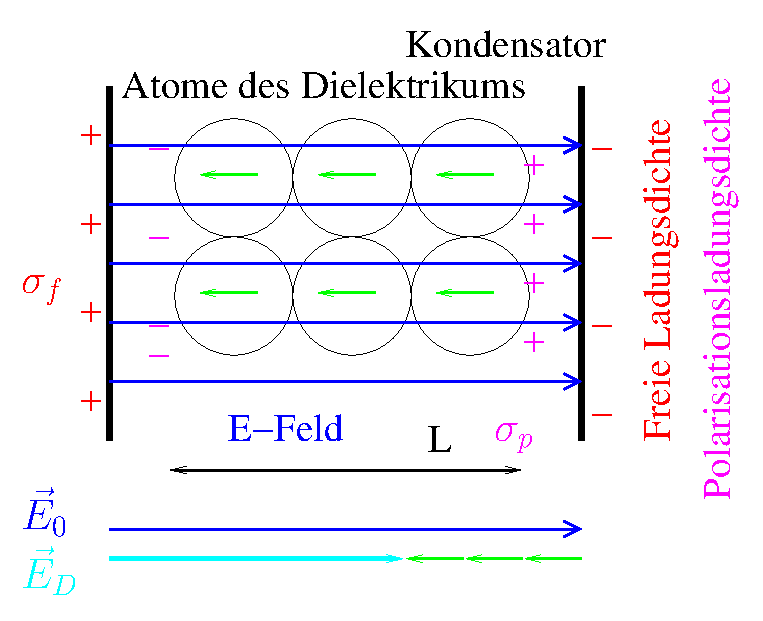
\includegraphics[width=0.7\textwidth]{bilder/dielektrikum}
   \caption[Polarisation im Dielektrikum]{Mikroskopische Betrachtung
     der Polarisation im Dielektrikum. Die Gr"unen Pfeile sind die
     $\vec p$}
   \label{abb_polarisation_dielektrikum}
\end{figure}


\bigskip

Mit dem Satz von \textsc{Gauss} (s. Kap. \ref{kap_satz-von-gauss})
gilt f"ur das au"sen anliegende E-Feld $\vec E_0$, weil die Ladungen auf
den Kondensatorplatten die Quellen des E-Felds $\vec E_0$ sind:
\begin{equation}
   \label{eqn_differenz-c36}
   E_0 = \frac{\sigma_f}{\varepsilon_0}
\end{equation}
Ist man nun am E-Feld $\vec E_D$ \emph{im Dielektrikum} interessiert,
so betrachtet man nur das Dielektrikum als Kondensator. Die
"`Platten"' (D-Platten) dieses Kondensators bestehen einmal aus dem
Rand des Dielektrikums mit der Ladung $\sigma_p$ und den
entsprechenden Platten des Kondensators mit der Ladung
$\sigma_f$. Weil die beiden Ladungen einander entgegengesetzt sind,
verwenden wir die \emph{Differenz} daraus als Ladungsdichte der
D-Platten. Wieder gilt mit \textsc{Gauss} und Gl. \eqref{eqn_differenz-c34}
\begin{equation}
   \label{eqn_differenz-c37}
   E_D = \frac{\sigma_f - \sigma_p}{\varepsilon_0} = \frac{\sigma_f -
     P}{\varepsilon_0} = E_0 -  \frac{P}{\varepsilon_0}
\end{equation}
Vergleicht man nun die St"arke der beiden E-Felder, indem man den
Quotienten bilden, erh"alt man (vgl. \eqref{eqn_def_espilon}):
\begin{equation}
   \label{eqn_differenz-c39}
   \frac{E_0}{E_D} = 1 + \frac{P}{E_D \cdot \varepsilon_0} =: 1 + \chi
   = \frac{U_0}{U_D} = \varepsilon_r
\end{equation}

Dabei haben wir eingef"uhrt:
\begin{Def}
   [\index{elektrische Suszeptibilit"at}Elektrische Suszeptibilit"at
   $\chi$] Ist ein anderes Ma"s f"ur die Polarisierbarkeit eines Stoffes
   unter einem au"sen angelegten E-Feld.
\end{Def}



Setzen wir in Gl. \eqref{eqn_differenz-c32} Gl. \eqref{eqn_differenz-c37} ein, erhalten wir
\begin{equation*}
   \label{eqn_differenz-c40}
    P = n \alpha \left (E_0 -  \frac{P}{\varepsilon_0} \right )
\end{equation*}
L"ost man diese Gleichung nach $P$ auf, erh"alt man mit
Gl. \eqref{eqn_def_espilon}:
\begin{equation*}
   \label{eqn_differenz-c41}
   P = \frac{n\alpha E_0}{1 + \frac{n\alpha}{\varepsilon_0}} =
 \frac{n\alpha E_D \varepsilon_r}{1 + \frac{n\alpha}{\varepsilon_0}} =
\underbrace{n \cdot \underbrace{\alpha \cdot E_D}_p}_{P} \cdot  \frac{\varepsilon_r}{1 + \frac{n\alpha}{\varepsilon_0}}
\end{equation*}
Ein Koeffizientenvergleich liefert also:
\begin{equation*}
   \label{eqn_differenz-c42}
    \frac{\varepsilon_r}{1 + \frac{n\alpha}{\varepsilon_0}} = 1 \text{
    und damit } 1 + \frac{n\alpha}{\varepsilon_0} = \varepsilon_r
\end{equation*}
und weiter mit Gl. \eqref{eqn_differenz-c39}
\begin{equation}
   \label{eqn_differenz-c43}
   \chi = \frac{n\cdot \alpha}{\varepsilon_0}
\end{equation}

\bigskip
Die drei Gr"o"sen $\alpha$, $\varepsilon_r$ und $\chi$ stehen also im
Zusammenhang
$$1 + \chi = \varepsilon_r \text{ und } \chi = \frac{n\cdot
  \alpha}{\varepsilon_0}$$

Damit kann man beispielsweise die Polarisation $\vec P$ in
Abh"angigkeit der E-Felder ausrechnen; dazu l"ost man die rechte
Gleichung nach $\alpha$ auf, die linke nach $\chi$, setzt das $\chi$
ein, und das dann wiederum in $\vec{{P}} = n \, \alpha \, \vec E_D$. Es folgt:
\begin{equation}
   \label{eqn_differenz-c44}
   \vec{{P}} = \varepsilon_0 \cdot ( \vec E_0 - \vec E_D) = \varepsilon_0 \cdot
   \left (1
   - \frac{1}{\varepsilon_r} \right ) \cdot \vec E_0 = \varepsilon_0 \cdot
 \underbrace{ (\varepsilon_r - 1) }_\chi \cdot \vec E_D
\end{equation}









\subsection{Arten von Polarisation}
\label{kap_arten-von-polarisation}

\begin{description}[\setlabelstyle{\bfseries\slshape}]
\item[\index{Verschiebungspolarisation}Verschiebungspolarisation] Verschiebung der Ladungsschwerpunkte
   durch ein "au"seres E-Feld induziert ein Induziertes Dipolmoment
   $\vec p = \alpha \cdot \vec E$ welches von der Temperatur abh"angig ist.
\item[\index{Orientierungspolarisation}Orientierungspolarisation] Die Molek"ule sind schon
   polarisiert (bspw. Wasser -- vgl Abb. \ref{abb_polares_wassermolekuel}) und werden
   durch ein externes E-Feld nur noch ausgerichtet. Bei h"oheren
   Temperaturen macht die thermische Bewegung der Molek"ule die
   Orientierung der Teilchen -- und damit auch die Polarisierung --
   schwer. Es gilt $$\|\vec p\| \sim \frac{1}{T}$$
\item[\index{Ionenpolarisation}Ionenpolarisation] Die beiden Gitter f"ur Kationen und Anionen
   werden gegeneinander verschoben; aus der Ladungsverschiebung
   resultiert ein Feld. S. Abb. \ref{abb_kristallgitter}
\item[\index{Ferroelektrika}Ferroelektrika] Die Kristalle besteht aus
   vielen Dipolen. Diese sind innerhalb von \emph{\index{Dom"anen}Dom"anen} (auch
   \index{Weiss-Bezirk}\textsc{Weiss}-Bezirke genannt) parallel
   ausgerichtet. Eine Dom"ane umfasst $10^6$ bis $10^9$ Atome und hat
   eine Ausdehnung zwischen $10^{-8}$ und $10^{-6}$m. Beim Anlegen
   eines "au"seren Feldes richten sich diese Zellen St"uck f"ur St"uck aus
   -- die Ausrichtung erfolgt nicht kontinuierlich, sondern
   sprunghaft.
\end{description}

\begin{figure}
   \centering
\subfigure[polares
Wassermolek"ul\label{abb_polares_wassermolekuel}]{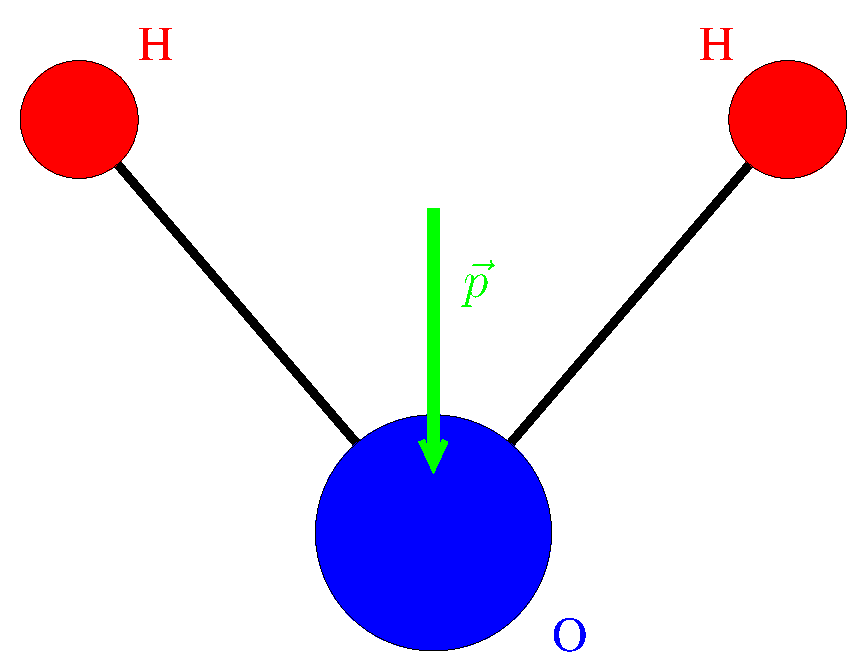
\includegraphics[width=0.35\textwidth]{bilder/wasser}}
\hfill
\subfigure[normales und verschobenes Kristallgitter\label{abb_kristallgitter}]{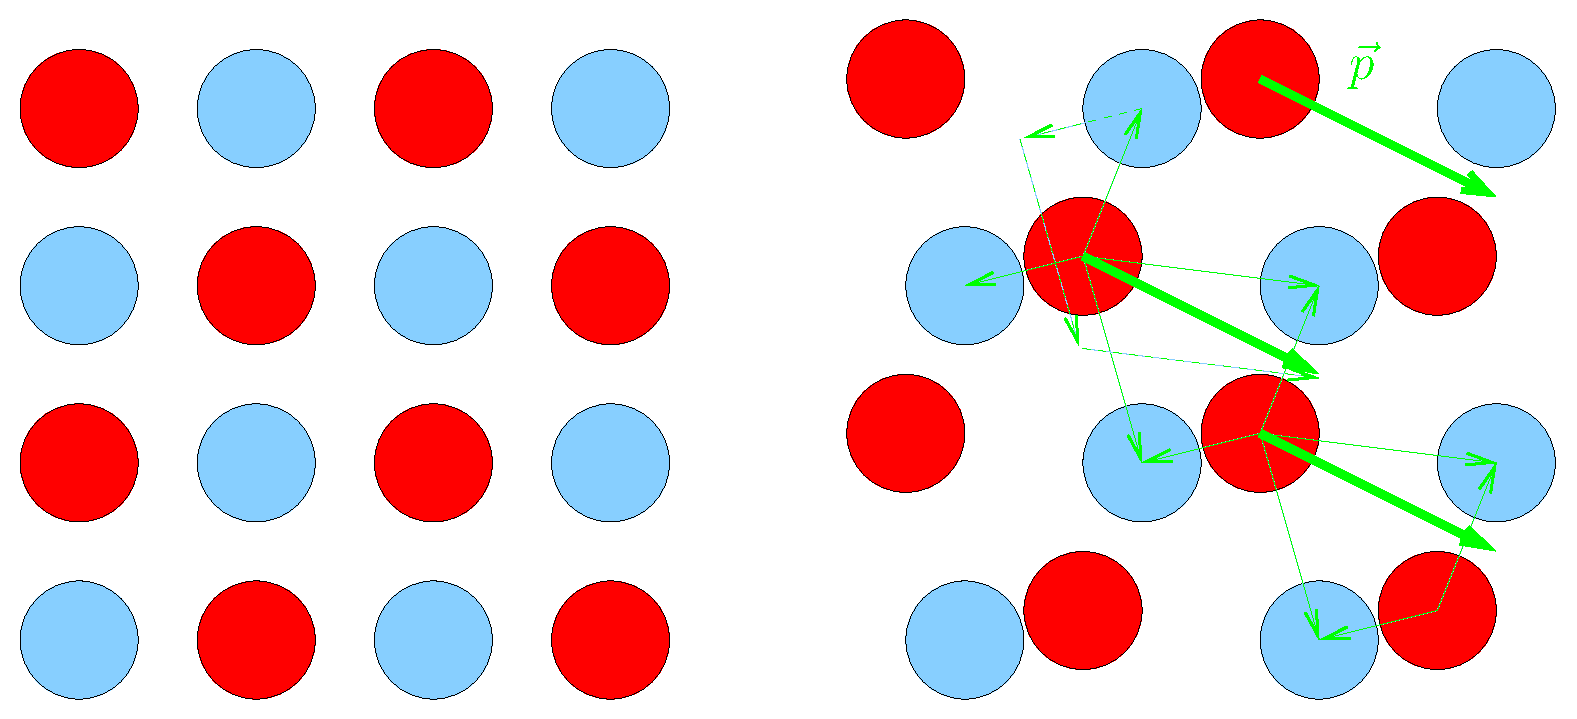
\includegraphics[width=0.6\textwidth]{bilder/kristallgitter}}
   \caption{Arten von Polarisation}
   \label{abb_polarisationsarten}
\end{figure}









\subsection{Elektrostatik in Dielektrika}
\label{kap_elektrostatik-in-dielektrika}

Wir hatten bisher homogene E-Felder betrachtet. Hier waren die
negativen und positiven Polarisationsladungen (bzw. $\sigma_p$) stets
gleich gro"s, sodass die \emph{Summe} der Polarisationsladungen
verschwand. Wir wollen jetzt aber ein \emph{inhomogenens} E-Feld
mit Dielektrikum betrachten; vgl. dazu Abb. \ref{abb_inhom_dielektr}.

Wenn man sich gem"a"s Abb. \ref{abb_polarisation_dielektrikum} versucht,
die einzelnen Dipole des Dielektrikums vorzustellen, so wird man bald
sehen, dass es in diesem Feld nicht m"oglich ist, dass die Dipole ihre
Ladungen gegenseitig zu Null ausgleichen: Auch innerhalb des
Dielektrikums wird es Ladungen geben. Somit sind die
Polarisationsladungen, die sich auf der Oberfl"ache bilden --
$\sigma_p^+$ und $\sigma_p^-$ -- verschieden gro"s und so kann man die
Ladung $Q$ bestimmen, die insgesamt auf der Oberfl"ache liegt. Dazu
integriert man "uber die Oberfl"ache $A$ und verwendet
Gl. \eqref{eqn_differenz-c34} und anschlie"send (bei $*$) den Satz von
\textsc{Gauss} (vgl. Kap. \ref{kap_satz-von-gauss})
\begin{equation}
   \label{eqn_differenz-c45}
   Q = \int_A \sigma_p \diff A = \int_A
   \vec P \cdot \diff \vec A
\stackrel{*}{=} \int_V \vec \nabla \vec P \diff V
\end{equation}

Da das Dielektrikum insgesamt neutral ist, muss im Inneren eine Ladung
$Q_P$ existieren mit
\begin{equation*}
   Q_p = -Q
\end{equation*}
Da diese sich irgendwo im \emph{Volumen} $V$ aufh"alt, integrieren wir
die Ladungsdichte im gesamten Volumen:
\begin{equation}
   \label{eqn_differenz-c46}
   Q_p = -Q = \int_V \varrho_p \diff V ~ \text{ bzw. } ~ Q = - \int_V
   \varrho_p \diff V
\end{equation}
Nun k"onnen wir mit Gl. \eqref{eqn_differenz-c45} einen Koeffizientenvergleich
anstellen und erhalten
   \begin{equation}
   \label{eqn_differenz-c47}
\boxed{   \vec \nabla \, \vec P = - \varrho_p   }
\end{equation}
\begin{Wichtig}
Die Polarisationsladungen im Dielektrikum sind die Quellen der Polarisation.
\end{Wichtig}
Vergleiche dazu auch $\vec \nabla \, \vec E =
\frac{\varrho}{\varepsilon_0}$ aus Kap. \ref{kap_satz-von-gauss}.



\begin{figure}
   \centering
   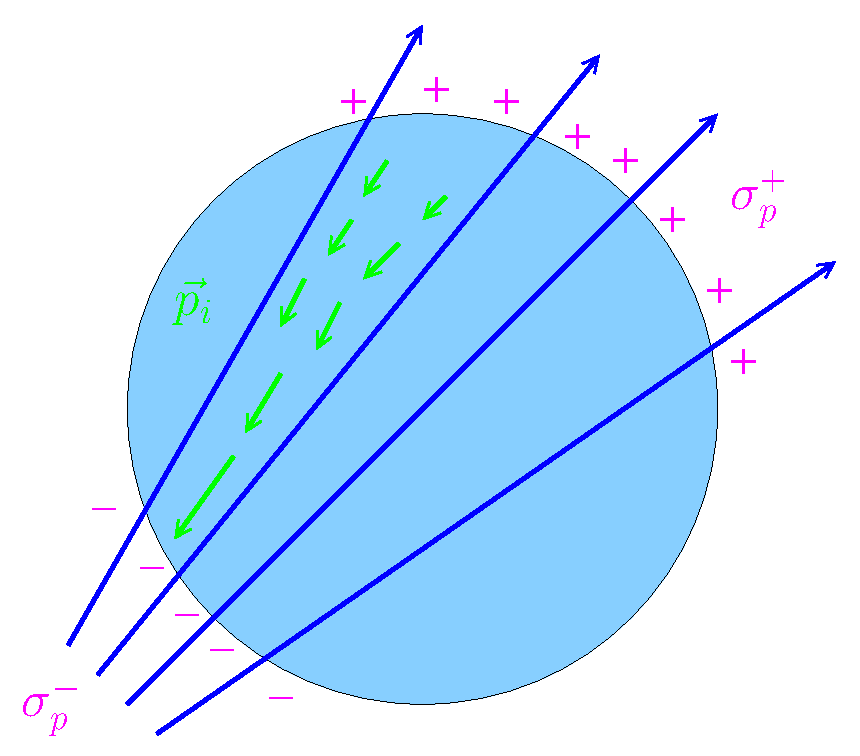
\includegraphics[width=0.7\textwidth]{bilder/inhom_dielektr}
   \caption{Dielektrikum in inhomogenem E-Feld}
   \label{abb_inhom_dielektr}
\end{figure}


\bigskip

Neben den Polarisationsladungen im Inneren kommen
(bzw. k"onnen kommen) noch weitere, \emph{freie} Ladungen im Inneren
mit der Dichte $\varrho_f$ hinzu, sodass die gesamte Ladungsdichte
sich zusammensetzt:
\begin{equation}
   \label{eqn_differenz-c48}
   \varrho = \varrho_p + \varrho_f
\end{equation}
Wenden wir nun wieder den Satz von \textsc{Gauss} an
(Kap. \ref{kap_satz-von-gauss}), erhalten wir:
% \begin{equation}
%    \label{eqn_differenz-c49}
%    \vec \nabla \, \vec E_D = \frac{\varrho_f + \varrho_p}{\varepsilon_0}
% \end{equation}
\begin{equation}
   \label{eqn_differenz-c50}
   \int_A \vec E_D \diff \vec A = \frac{1}{\varepsilon_0} \int_V
   \varrho \diff V
=
\frac{1}{\varepsilon_0} \int_V (\varrho_f + \varrho_p) \diff V =
\frac{1}{\varepsilon_0} \int_V \varrho_f\diff V + \frac{1}{\varepsilon_0} \int_V \varrho_p \diff V
\end{equation}
und mit Gl. \eqref{eqn_differenz-c46} und \eqref{eqn_differenz-c45}
\begin{equation*}
   \label{eqn_differenz-c51}
     \int_A \vec E_D \diff \vec A  = \frac{1}{\varepsilon_0} \int_V
     \varrho_f\diff V  - \frac{1}{\varepsilon_0}\int_A \vec P \diff \vec A
\end{equation*}
Dies kann man wegen der Linearit"at des Integrals und mit
Gl. \eqref{eqn_differenz-c37} umformen zu
\begin{equation}
   \label{eqn_differenz-c52}
   \int_A \left (\vec E_D + \frac{\vec P}{\varepsilon_0}\right )
   \diff \vec A = \int_A \vec E_0 \diff \vec A =
\frac{1}{\varepsilon_0}   \int_V \varrho_f \diff V = \frac{Q_f}{\varepsilon_0}
\end{equation}
Multipliziert man dies mit $\varepsilon_0$, so kann man einf"uhren:
\begin{Def}
   [\index{Elektrische Flussdichte}Elektrische Flussdichte $\vec D$]
   oder \index{D-Feld}\index{Dielektrische
     Verschiebung}"`Dielektrische Verschiebung"'
   \begin{equation}
      \label{eqn_differenz-c53}
      \boxed{  \vec D = \varepsilon_0 \cdot \vec E_D + \vec P =
        \varepsilon_0 \cdot \varepsilon_r \cdot \vec E_D =
        \varepsilon_0 \cdot \vec E_0  }
   \end{equation}
Das D-Feld kann man sich vorstellen als das E-Feld, welches nur von
den \emph{freien} Ladungen erzeugt wird, w"arend das E-Feld von
\emph{allen} Ladungen erzeugt wird.
\end{Def}
Man kan dies schreiben als
\begin{equation}
   \label{eqn_differenz-c55}
   \vec \nabla \, \vec D = \varrho_f
\end{equation}
Dies entspricht genau Gl. \eqref{eqn_differenz-c52}, wenn man mit $\varepsilon_0$
multipliziert, den Satz von \textsc{Gauss} anwendet und einen
Koeffizientenvergleich macht.

Das D-Feld besteht aus dem E-Feld $\vec E_D$ im Dielektrikum und der
Polarisation $\vec P$. Deswegen hat es auch die Einheit der
Polarisation oder Fl"achenladungsdichte: $[\vec D] =
 \frac{\operatorname{C}}{\operatorname{m}^2}  =
 \frac{\operatorname{As}}{\operatorname{m}^2}$.

 \begin{Wichtig}
    In Materie gilt also
    \begin{equation}
       \label{eqn_differenz-c54}
       \boxed{ \int_A \vec E \diff \vec A = \frac{Q_f +
           Q_p}{\varepsilon_0}   }
    \end{equation}
Diese Schreibweise ist allgemeiner, weil ohne Materie keine Ladungen
polarisiert werden k"onnen und damit $Q_p$ verschwindet.
 \end{Wichtig}





\subsection{Brechungsgesetz $(\bigstar)$}
\label{kap_brechungsgesetz}

Wir betrachten die Grenzfl"ache zwischen zwei Materialien an die ein
E-Feld angelegt werde. Der E-Feldvektor habe im ersten Material den
Winkel $\alpha$ zur Fl"achennormalen. Wir bezeichnen die E-Felder mit
$\vec E'$ und $\vec E''$ und analog die Felder in Materie $\vec E_D$
und die relativen Permittivit"aten $\varepsilon_r$. Es sei
\begin{equation}
\label{eqn_differenz-c57}
   \varepsilon_r'' < \varepsilon_r'
\end{equation}
 Vlg. dazu Abb. \ref{abb_brechung}.

\begin{figure}
   \centering
   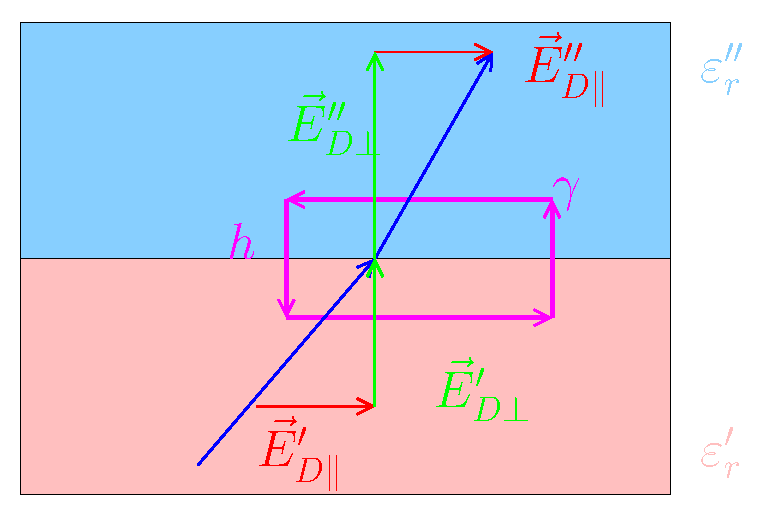
\includegraphics[width=0.7\textwidth]{bilder/brechung}
   \caption{Brechung eines E-Felds beim Phasen"ubergang mit
     $\varepsilon_r'' < \varepsilon_r'$}
   \label{abb_brechung}
\end{figure}
Wir betrachten nun das E-Feld komponentenweise:
\begin{description}[\setlabelstyle{\bfseries\slshape}]
\item[Senkrecht zum Phasen"ubergang $\vec E_{D \bot}$] Wie wir in
   Kap. \ref{kap_isolatoren-im-e-feld} gesehen haben, gilt
   \begin{equation}
      \label{eqn_differenz-c56}
\vec E_{0 \bot}  =  \varepsilon_r' \cdot \vec E_{D \bot}' = \varepsilon_r'' \cdot \vec E_{D \bot}''
   \end{equation}
   D.h. mit \eqref{eqn_differenz-c57} wissen wir, dass $\vec E_{D \bot}''$
   \emph{gr"o"ser} sein muss, als $\vec E_{D \bot}'$ und zwar um den
   Faktor
   \begin{equation}
\label{eqn_differenz-c60}
      n = \frac{\varepsilon_r'}{\varepsilon_r''} \text{ womit } E_{D
        \bot}'' = n \cdot E_{D \bot}'
   \end{equation}

\item[Parallel zum Phasen"ubergang $\vec E_{D \|}$] Dazu bilden wir
   ein geschlossenes Ringintegral "uber $\gamma$ (vgl. wieder
   Abb. \ref{abb_brechung}), wobei $h = o(1)$ sein soll -- also
   verschwindend klein:
   \begin{equation}
      \label{eqn_differenz-c58}
      \oint_\gamma \vec E \diff s =
 \int_\text{hin} E_{D \|}' \diff s_\text{hin} +  \int_\text{r"uck} E_{D
   \|}'' \diff s_\text{r"uck} + o(1)
   \end{equation}
   Wobei $s_\text{hin}$ der untere lila Pfeil ist, also die Strecke im
   ersten Medium. Da das E-Feld wirbelfrei ist, muss dieser Ausdruck
   verschwinden. Da au"serdem $\gamma$ so gew"ahlt ist, dass
   \begin{equation*}
      \gamma_\text{hin} = \gamma_\text{r"uck} \text{ bzw. } \diff
      s_\text{hin} = \diff s_\text{r"uck}
   \end{equation*}
   folgt sofort
   \begin{equation}
      \label{eqn_differenz-c59}
      E_{D \|}' = E_{D \|}''  \text{ bzw. } \vec E_{D \|}' = \vec E_{D \|}''
   \end{equation}
\end{description}

Wenn $\vec E_D'$ also unter
\begin{equation*}
\tan \alpha =  \frac{E_{D \|}'}{E_{D \bot}'}
\end{equation*}
einf"allt, so wird $\vec E_D''$ ausfallen unter $\beta$ (mit $n$ aus
Gl. \eqref{eqn_differenz-c60} und Gl. \eqref{eqn_differenz-c59}):
\begin{equation*}
   \tan \beta =
 \frac{E_{D \|}''}{E_{D \bot}''}
=
 \frac{E_{D \|}'}{n \cdot E_{D \bot}'}
=
\frac{1}{n} \cdot \tan \alpha
\text{ ~ oder } \boxed{  \tan \alpha = n \cdot \tan \beta }
\end{equation*}
Dabei haben wir mit $n$ den
\textbf{\index{Brechungsindex}Brechungsindex} eingef"uhrt:
\begin{Def}
   [Brechungsindex oder Brechzahl $n$] ist eine Gr"o"se f"ur die
   Richtungs"anderung von Licht (oder hier einem E-Feld) beim "Uberganz
   zwischen zwei Materialien.
\end{Def}













\section{Der Elektrische Strom}
\label{kap_elektrische-strom}

\subsection{Stromst"arke und Stromdichte}
\label{kap_stromstarke-und-stromdichte}

\begin{Def}
   [\index{Stromst"arke}Stromst"arke $I$]
   \begin{equation}
      \label{eqn_differenz-c61}
      I = \frac{\diff Q}{\diff t} = \dot Q
   \end{equation}
Die Stromst"arke ist die Ladungsmenge die pro Zeiteinheit durch die zur
Stromrichtung senkrecht stehende Querschnittsfl"ache des Leiters flie"st.
\end{Def}
Mit der Einheit $[I] = A = \frac{\operatorname{C}}{\operatorname{s}}$.
Die Einheit ist eine der fundamentalen Einheiten des
\index{MKS-System}MKS-Systems (vgl. Kap. \ref{kap_mks-system}); ihre
Definition ist deshalb entscheidend:\footnote{Die Leiter liegen
  parallel angeordnet im Abstand von einem Meter im Vakuum und werden
  mit Strom beschickt. Sie bilden B-Felder aus, welche sich
  durchdringen, verst"arken und so die Dr"ahte einander anziehen. Der
  Strom wird so reguliert, dass die beiden Dr"ahte pro Meter eine
  Kraft von $2\cdot 10^{-7}\operatorname{N}$ aufeinander aus"uben --
  der Strom hat dann per Definition die St"arke $1\operatorname{A}$.}
\begin{quote}
   1 \index{Amp\`ere}Amp\`ere ist die St"arke eines zeitlich
   konstanten Stromes, der zwischen zwei parallelen, unendlich langen,
   im Vakuum liegenden Leitern, die im Abstand von 1 m angeordnet
   sind, die Kraft von $2 \cdot 10^{-7} \operatorname{N}$ pro Meter
   Leitungsl"ange bewirkt.
\end{quote}

Neben der Strom\emph{st"arke} ben"otigen wir auch die
Strom\emph{dichte}:
\begin{Def}
   [\index{Stromdichte}Stromdichte $\vec j$] Die Stromdichte ist der
   Quotient von Stromst"arke pro Fl"ache:
   \begin{equation}
      \label{eqn_differenz-c62}
      j = \frac{I}{A}
   \end{equation}
   und zeigt als Vektor in Richtung der Stromrichtung. ($\to$
   \emph{\index{Pointing-Vector}Pointing-Vector}) 
\end{Def}
Die Einheit der Stromdichte ist $[\vec j] = [j] =
\frac{\operatorname{A}}{\operatorname{m}^2}$.

Die Ladung $Q$ in einem Leitervolumen $V$ ist $\varrho \cdot A \cdot
x$ und mit der Ladungstr"agerdichte $n$ und der Ladung $q$ eines
Ladungstr"agers kommt man auf $n \cdot q \cdot A \cdot x$. Um nun die
Strom\emph{st"akre} zu bestimmen, braucht man dies nur zeitlich
abzuleiten. F"ur die Strom\emph{dichte} teilt man anschlie"send durch
$A$:
\begin{equation}
   \label{eqn_differenz-c63}
   \frac{\diff (n \cdot q \cdot A \cdot x)}{A \cdot \diff t}
=
   \frac{n \cdot q \cdot A }{A} \cdot \frac{\diff x}{\diff t}
=
\boxed{  n \cdot q \cdot \vec v_d = \varrho \cdot \vec v_d = \vec j}
\end{equation}
Hier bezeichnet $\vec v_d$ die
\emph{\index{Driftgeschwindigkeit}Driftgeschwindigkeit}, mit der sich
die Ladungstr"ager durch den Leiter bewegen.

Ein wichtiger \textbf{Zusammenhang} zwischen Stromst"arke und -dichte
ist:
\begin{equation}
   \label{eqn_zshg_stromstaerke-stromdichte}
   \boxed{ I = \int_A \vec j \diff \vec A  }
\end{equation}
Dabei ist $I$ der gesamte Strom\footnote{Man kann deshalb $I$ auch als
  \emph{\index{Stromfluss}Stromfluss} bezeichnen; dabei ist der
  Begriff \emph{Fluss} aus der Feldtheorie, in der Allgemein $\Phi =
  \int_A \vec \phi \diff \vec A$ mit einem Allgemeinen Fluss $\Phi$
  und einer allgemeinen Flussdichte $\vec \phi$.} durch die Fl"ache
$A$. Ist die Stromdichte r"aumlich konstant und ist $\vec A$ parallel
zu $\vec j$ vereinfacht
% \footnote{Diese
%   Vereinfachung gilt, weil nach Definition $A$ stets senkrecht zu
%   $\vec j$ ist und damit $\vec A$ stets parallel zu $\vec j$ ist.}
sich dies zu
\begin{equation*}
   I = \vec j \cdot \vec A = j \cdot A
\end{equation*}


\bigskip

\begin{Wichtig} [Ursache des Stroms]
   Eine Voraussetzung daf"ur, dass Strom flie"sen kann, ist die
   Anwesenheit von Spannung.
\end{Wichtig}
Die Spannung $U$ ist eine \emph{Potentialdifferenz} $\Delta \varphi$
(vgl. \eqref{eq:184}: Ladungen bewegen sich an die Stelle niedrigeren
(elektrischen) Potentials. Diese Bewegung von Ladung bezeichnen wir
als Strom.


\begin{Wichtig}
   Wir vernwenden als Stromrichtung die \textbf{konventionelle} oder
   \emph{technische} \textbf{\index{Stromrichtung}Stromrichtung}:
   Strom flie"st von Plus nach Minus.
\end{Wichtig}
Mit dieser Vereinbarung ist Strom und bspw. E-Feld besser vereinbar.


\subsection{Exkurs: Kontinuit"atsgleichung $(\bigstar)$}
\label{kap_exkurs:-kontinuitatsgleichung}

Wendet man auf $\oint_A \vec j \diff \vec A$ den Satz von
\textsc{Gauss} (vgl. Kap. \ref{kap_satz-von-gauss}) an, so ist
\begin{equation}
   \label{eqn_differenz-c65}
 I = \oint_A \vec j \diff \vec A = \int_V \vec \nabla \, \vec j \diff V
\end{equation}
Wir betrachten nun ein Volumen $V$, welches die Ladung $Q = Q(t)$
enth"alt bzw. die Ladunngsdichte $\varrho = \varrho(\vec r,t)$ mit
\begin{equation*}
   Q(t) = \int_V \varrho(\vec r, t) \diff V
\end{equation*}
Wenn nun Ladung aus dem Volumen \emph{heraus}flie"st, so wird $Q$
\emph{kleiner}. Dies f"uhrt also dazu, dass an der Oberfl"ache $A
= \partial V$ Strom mit \emph{positiver} St"arke austritt. Damit ist
also an der Oberfl"ache
\begin{equation}
   \label{eqn_differenz-c67}
    I = - \frac{\diff Q}{\diff t} = -\frac{\diff }{\diff t} \int_V
   \varrho(\vec r,t) \diff V = -\int_V \frac{\partial \varrho(\vec
     r,t)}{\partial t} \diff V
\end{equation}
Vergleicht man das mit Gl. \eqref{eqn_differenz-c65}, so sieht man sofort
\begin{equation}
   \label{eqn_differenz-c64}
   \boxed{ \vec \nabla \, \vec j(\vec r,t) = - \frac{\partial }{\partial t}
     \varrho(\vec r,t)  }
\end{equation}
oder auch\footnote{unter Misshandlung des $\partial$-Operators}:
\begin{equation*}
   \frac{\partial \vec j}{\partial \vec r} = - \frac{\partial \varrho}{\partial t}
\end{equation*}
In Worten bedeutet dies:
\begin{Wichtig}[\index{Kontinuit"atsgleichung}Kontinuit"atsgleichung]
   Die Ladungsverteilung in einem Volumen (rechte Seite) kann sich
   ausschlie"slich durch Verschiebung der Ladung "andern: Es kann keine
   Ladung erzeugt oder vernichtet werden!
\end{Wichtig}






\subsection{Elektrischer Widerstand}
\label{kap_elektrischer-widerstand}

\begin{Def}
   [\index{Widerstand}Widerstand $R$] ist ein Ma"s daf"ur, welche
   Spannung $U$ erforderlich ist, um den Strom $I$ durch ein Material
   flie"sen zu lassen.
   \begin{equation}
      \label{eqn_differenz-c66}
      R = \frac{U}{I}
   \end{equation}
\end{Def}
Die Einheit des Widerstandes ist $[R] = \Omega =
\frac{\operatorname{V}}{\operatorname{A}}$ (Ohm), als
\index{Schaltsymbol!Widerstand}Schaltsymbol verwendet man einen
Kasten.

\begin{Wichtig}
   [\index{Ohm'sches Gesetz}\textsc{Ohm}'sches Gesetz] $R$ ist
   konstant und nur vom Material abh"angig.
\end{Wichtig}

Leider ist dieses Gesetz nicht allgemeing"ultig, sondern ist nur eine
\emph{N"aherung} bei (relativ) kleinen Stromst"arken. Siehe auch
Kap. \ref{kap_mechanismen-elektrischer-leiter} und weiter unten.

\bigskip

Die \textbf{Ursache} f"ur einen Widerstand $R$ ist, dass Ladungstr"ager
von dem Medium, in dem sie leiten \emph{ausgebremst} werden: Sie
sto"sen mechanisch oder erfahren Anziehungskr"afte. Diese Effekte sind
mit einer Reibung zu vergleichen, die dem Vorankommen der
Ladungstr"ager entgegenwirkt. Die Ladungstr"ager erreichen so eine
mittlere Geschwindigkeit, als
\textbf{\index{Driftgeschwindigkeit}Driftgeschwindigkeit} $v_d$
bezeichnet. Sie ist proportional zur Kraft, mit der die Ladungstr"ager
bewegt werden, also
\begin{equation}
   \label{eqn_differenz-c71}
   v_d \sim F = q \cdot E
\end{equation}
Mit Gl. \eqref{eqn_differenz-c63} ist dies auch proportional zur Stromdichte
$j$. Die Proportionalit"atskonstante ist:
\begin{Def}
   [\index{Leitf"ahigkeit}(\index{elektrische
     Leitf"ahigkeit}elektrische) Leitf"ahigkeit $\sigma$] (oder
   \index{Konduktivit"at}"`Konduktivit"at"') Gibt an, wie gut ein
   Stoff Strom leitet, wenn ein E-Feld anliegt.
   \begin{equation}
      \label{eqn_differenz-c72}
      \vec j = \sigma \cdot \vec E
   \end{equation}
\end{Def}
\footnote{Im Allgemeinen Fall ist $\Ten \sigma$ ein Tensor! D.h. dass
  die Richtung von $\vec j$ und $\vec E$ nicht unbedingt parallel sein
  m"ussen. Beispiele daf"ur sind Materialien mit Schichtstruktur wie
  Graphit.}Die Einheit der Leitf"ahigkeit ist $[\sigma] = \frac{1}{\Omega
  \cdot \operatorname{m}}$.

Den Kehrwert der Leitf"ahigkeit bezeichnet man auch als
\textbf{\index{Spezifischer Widerstand}Spezifischen Widerstand}
$\rho_\Omega$ oder $\rho$. Dessen Einheit ist $[\rho] = [\rho_\Omega]
= \Omega \cdot \operatorname{m}$:
\begin{equation}
   \label{eqn_differenz-c74}
   \sigma = \frac{1}{\rho}
\end{equation}

\begin{Wichtig}
   Sowohl $\sigma$ als auch $\rho$ sind \emph{Materialkonstanten}.
\end{Wichtig}

Aus dem Spezifischen Widerstand kann man den Widerstand eines K"orpers
der L"ange $L$ und Querschnittsfl"ache $A$ bestimmen:
\begin{equation}
   \label{eqn_differenz-c73}
   R = \rho \cdot \frac{L}{A}
\end{equation}
In Tab. \ref{tab_spez_widerst} sind ein paar Werte f"ur $\rho$ f"ur
verschiedene Materialien aufgelistet.

\begin{table}
   \centering
   \begin{tabular}{l l}
\toprule
      \textbf{Material} & \textbf{$\rho$ in $\frac{\Omega \cdot
          \operatorname{mm^2}}{\operatorname{m}}$} \\
\midrule
Quecksilber & 0.96\\
Blei & 0.21 \\
Stahl & 0.13 \\
Platin & 0.105\\
Eisen & 0.098 \\
Gold & 0.022 \\
Kupfer & 0.0172\\
Silber & 0.0163\\
\toprule
\textbf{Material} & \textbf{$\rho$ in $ \Omega \cdot \operatorname{m}$}\\
\midrule
Seewasser & 0.3\\
Flusswasser & $10-100$\\
destilliertes Wasser & $10^{4} - 4 \cdot 10^4$\\
reines Wasser in Vakuum & $2.5 \cdot 10^{5}$\\
\bottomrule
   \end{tabular}
   \caption{Spezifische Widerst"ande ausgew"ahlter Materiialien bei $20^\circ$C}
   \label{tab_spez_widerst}
\end{table}

\bigskip

Die \textbf{Temperaturabh"angigkeit} des Spezifischen Widerstands
dr"uckt man bei einem normalen metallischen Leiter durch
materialabh"angige Temperaturkoeffizienten $\alpha$ und $\beta$ aus mit
\begin{equation}
   \label{eqn_differenz-c75}
   \rho = \rho_{20} \cdot \left (1 + \alpha \cdot (\vartheta - 20) + \beta
      \cdot (\vartheta - 20)^2 \right )
\end{equation}
wobei $\vartheta$ die Temperatur in Grad Celsius ist und $\rho_{20}$ der
spezifische Widerstand. F"ur kleine $\alpha$ und $\beta$ oder f"ur nur
kleine Temperaturabweichungen von $20^\circ\operatorname{C}$ kann man
diese Korrekturfaktoren vernachl"assigen. Siehe dazu auch
Abb. \ref{abb_spez_widerst_temp}. Hier sieht man die quadratischen
Korrekturen kaum...

\begin{figure}
   \centering
   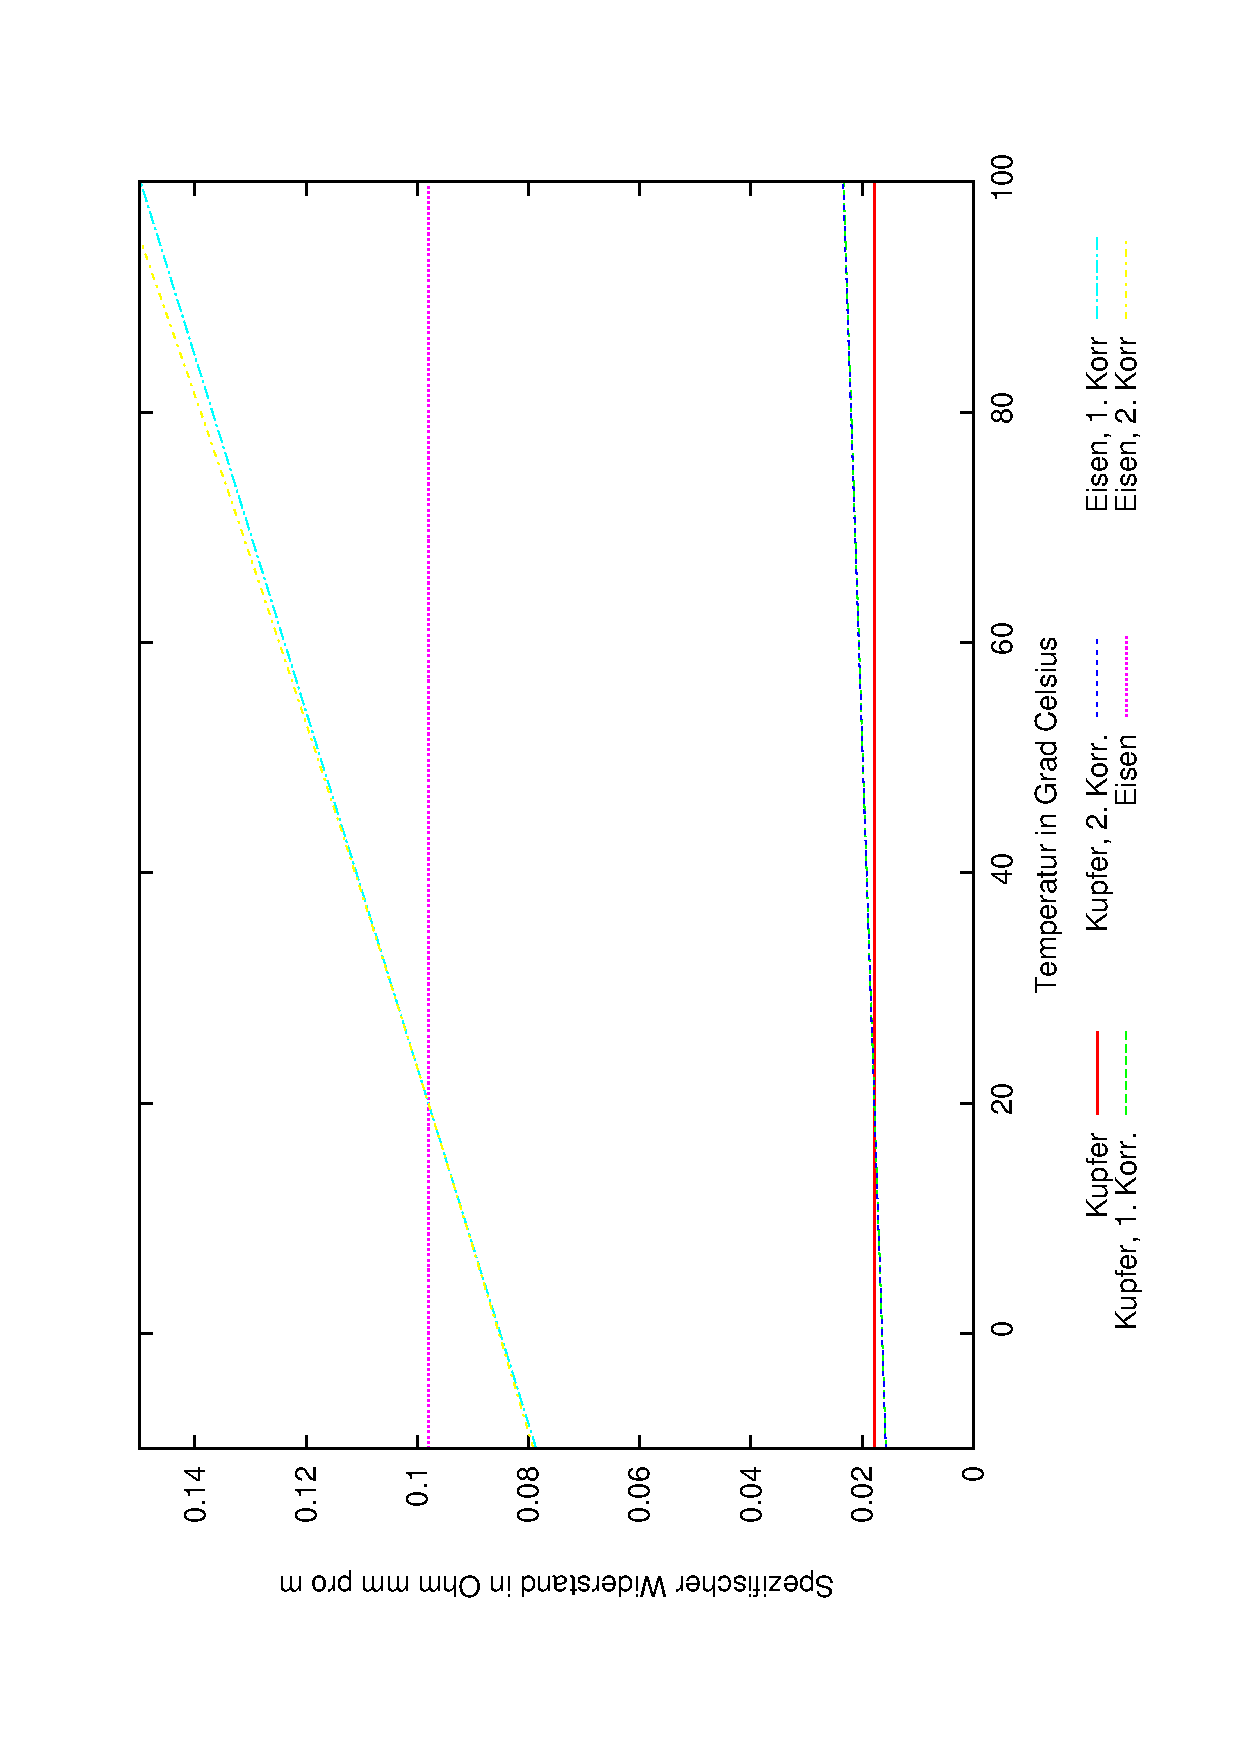
\includegraphics[angle=-90,width=\textwidth]{bilder/spez_widerst}
   \caption{Temperaturabh"angigkeit des Widerstandes von Eisen und kupfer}
   \label{abb_spez_widerst_temp}
\end{figure}












\subsection{Mechanismen elektrischer Leiter}
\label{kap_mechanismen-elektrischer-leiter}

\begin{description}[\setlabelstyle{\bfseries\slshape}]
\item[Festk"orper] Die Atome des K"orpers sind (mehr oder weniger) starr
   miteinander verbunden und damit ortsfest.
   \begin{description}[\setlabelstyle{\bfseries\slshape}]
   \item[Reine Metalle] Sehr gute Leiter: Die Elektronen sind v"ollig
      delokalisiert; Die Elektronen geben ihre Valenzelektronen in ein
      \emph{Elektronengas}. Hier sind die Elektronen frei beweglich.

      Der Widerstand ist (stark) \emph{temperaturabh"angig}: Bei tiefen
      Temperaturen ist er klein, bei steigenden Temperaturen w"achst
      auch der Widerstand: Je gr"o"ser die Temperatur, desto st"arker ist
      die Thermische Bewegung der Atomr"umpfe und desto gr"o"ser die
      Reibung, die den Elektronen entgegengesetzt ist; die Elektronen
      werden st"arker gestreut.
   \item[Supraleiter] Bei einer bestimmten Temperatur $T_C$
      ("`\index{Kritische Temperatur}Kritische Temperatur"' oder
      "`\index{Sprungtemperatur"'}Sprungtemperatur"' genannt) sinkt
      der Widerstand mit tieferen Temperaturen schlagartig auf exakt
      $0$ und bleibt bei $0$.
   \item[Halbleiter] Die Zahl der Ladungstr"ager, die auch wirklich
      \emph{leiten} h"angt von der Temperatur stark ab: SIe m"ussen mit
      einer bestimmten Energie angeregt werden, damit sie vom
      \emph{\index{Valenzband}Valenzband} (wo sie nicht leiten k"onnen)
      ins \emph{\index{Leitungsband}Leitungsband} gehoben werden (wo
      sie leiten).
   \item[Isolator] Hat keine freien Elektronen; diese sind an
      Atomr"umpfe gebunden; bei hohen Temperaturen trotzdem leitf"ahig.

      \begin{Beispiel}
      Bspw. flie"st bei Glas Strom, wenn man es auf
      $500^\circ\operatorname{C}$ erw"armt hat: Glasionen werden frei
      beweglich. Ab dann wird wegen ders gro"sen Widerstands des Glases
      durch die Reibungsw"arme der Ionen das Glas weiter erw"armt, bie
      es schmilzt.
      \end{Beispiel}
   \end{description}
\item[Fl"ussigkeiten] Bei reinem Wasser ist die Leitf"ahigkeit
   klein. Nur mit Salzen (Ionen) ist die Leitf"ahigkeit gr"o"ser. Bei
   Fl"ussigkeiten ist Stromleitung allgemein mit
   \emph{Material}transport verbunden.
   \begin{description}[\setlabelstyle{\bfseries\slshape}]
   \item[Elektrolyse] Kommen in einer L"osung Salzionen an die
      Elektroden, findet \textbf{\index{Elektrolyse}Elektrolyse}
      statt. Nach dem \textbf{\index{Faraday'sches
          Gesetz}Faraday}'schen Gesetz braucht man die Ladung $Q$ um
      $N$ Mole von $z$-wertig geladene Ionen zu elektrolysieren:
      \begin{equation*}
         Q = \mathrm F \cdot z \cdot N
      \end{equation*}
      mit der \textsc{\index{Faraday'sche Konstante}Faraday}'schen
      Konstante\footnote{Diese Konstante ist das Produkt zweier
        Konstanten: $\mathrm F = N_A \cdot e$ wobei $N_A$ die
        \textsc{\index{Avogadro-Konstante}Avogadro}-Konstante ist
        (Anzahl von Teilchen in einem Mol: $N_A = 6.022 \cdot
        10^{23}\frac{1}{\operatorname{mol}}$) und $e$ die
          Elementarladung $e = 1.602 \cdot 10^{-19}\operatorname{C}$ ist.} $\mathrm F = 96\,
      485\frac{\operatorname{C}}{\operatorname{mol}}$
   \item[Zusammenhang Strom, Spannung] Die Ionen erfahren die
      \textsc{Stokes}'sche Reibung
      (vgl. Kap. \ref{kap_stromende-flussigkeiten-und-gase})
      \begin{equation}
         \label{eqn_differenz-c68}
         F_R = 6 \pi \eta r \cdot v
      \end{equation}
      und ein Elektron erf"ahrt im E-Feld die Kraft
      \begin{equation}
         \label{eqn_differenz-c69}
         F_{el} = E \cdot e
      \end{equation}
      In der L"osung wird sich nach kurzer Zeit ein Gleichgewicht
      einstellen, sodass
      \begin{equation}
         \label{eqn_differenz-c70}
         6 \pi \eta r \cdot v = E \cdot e \text{ und damit ~} v =
         \frac{E \cdot e}{6 \pi \eta r} = \frac{U \cdot
           e}{\varepsilon_r \cdot d \cdot 6 \pi \eta r }
      \end{equation}
      und da $I \sim v$ ist somit auch $I \sim U$ -- das
      \textsc{Ohm}'sche Gesetz gilt also!
   \end{description}
\item[Gase] In einem Elektrolyt werden die Ladungstr"ager durch eine
   \index{Hydrath"ulle}Hydrath"ulle  stabilisiert: Diese sorgt daf"ur,
   dass die Ionen nicht sofort zu einem Salz rekombinieren k"onnen. In
   Gasen fehlt dieser Stabilisierungsmechanismus: Die Ionen
   rekombinieren sofort. Damit ein Gas Leitf"ahig ist, m"ussen st"andig
   neue Ionen gebildet werden.

\begin{Beispiel}
    \textbf{\index{Glimmlampe}Glimmlampe}. An einem Gasgemisch
      liegen an zwei Seiten Kontakte, die gegeneinander isoliert
      sind.  Durch eine Hohe Spannung werden Ionen und freie
      Elektronen erzeugt,  durch das E-Feld werden die Elektronen
      beschleunigt und  die Elektronen sto"sen an andere Atome
      und l"osen hier Ionen aus; dieser Vorgang hei"st
      "`\index{Sto"spolarisation"'}Sto"spolarisation"'. Dadurch sind
      st"andig neue Ionen vorhanden.

      Die eigentliche Leuchterscheinung kommt dadurch zustande, dass
      die Atome teilweise nicht ionisiert, sondern "`nur"' angeregt
      werden und diese Anregungsenergie als Photonen ($E = h \cdot
      \nu$) abgeben.

\bigskip

      \textbf{\textsc{\index{Geigerz"ahler}Geiger}-\textsc{M"uller}-Z"ahler}:
      In einem Metallrohr befindet sich ein Gas. Die Seitenfl"achen des
      Rohrs sind Isolatoren und in der Rohrmitte ist ein Draht
      gespannt. Dieser wird gegen das Rohr positiv geladen und der
      Strom im Draht wird gemessen.

      Tifft ein Radioaktives Teilchen ein, ionisiert dieses
      Gasteilchen. Die positiven Anionen werden zum negativen Rohr,
      die Ionen zum positiven Draht gezogen. Es findet jeweils ein
      Ladungsausgleich statt und auf dem Draht ist ein Strom zu
      messen.
\end{Beispiel}
\end{description}






\subsection{Stromkreis und Schaltungen}
\label{kap_stromkreis-und-schaltungen}

Komplizierte Schaltungen lassen sich zerlegen. Dazu fasst man
Verbraucher bzw. Widerst"ande zu
\emph{\index{Ersatzwiderst"anden}Ersatzwiderst"ande} zusammen. Es gibt
daf"ur zwei grundlegende M"oglichkeiten
(vgl. Abb. \ref{abb_schaltung_widerstaende}).
\begin{description}[\setlabelstyle{\bfseries\slshape}]
\item[Serienschaltung] Zwei Widerst"ande sind direkt hintereinander
   geschaltet: Der Strom, der durch den einen flie"st, flie"st auch
   durch den anderen. Dementsprechend ist $I$ auch in beiden
   gleich. Die Spannung dagegen Teilt sich auf. Betrachtet man das
   Potential, so muss, damit ein Strom flie"st, au"sen zwischen den
   Widerst"anden eine Potentialdifferenz anliegen, ebenso eine
   Differenz zwischen den "au"seren Enden und der Verbindung der
   Widerst"ande. Diese "`k"urzeren"' Potentialdifferenzen addieren sich
   zur gesamten. Bezeichnen wir die einzelnen Widerst"ande mit $R_1$
   und $R_2$ und entsprechend ihre Stromst"arken und Spannungen und mit
   $R_0$ den Ersatzwiderstand des Systems, gilt
   \begin{equation}
      \label{eqn_strom,spannung_reihe}
      I_1 = I_2 = I_0 \text{ und } U_1 + U_2 = U_0
   \end{equation}
   und damit
   \begin{equation}
      \label{eqn_widerstand_reihe}
      R_0 = \frac{U_0}{I_0} = \frac{U_1}{I_0} + \frac{U_2}{I_0} =
      \boxed { R_1 + R_2 = R_0 }
   \end{equation}
\item[Parallelschaltung] Hier muss sich der Strom beim flie"sen
   \emph{aufteilen} -- er kann das Potentialgef"alle entweder durch
   $R_1$ oder durch $R_2$ passieren. Da keine Ladung auf dem Weg
   verloren gehen darf, m"ussen die Stromst"arken sich addiern. Daf"ur
   ist aber das Potentialgef"alle -- und damit die Spannung -- auf
   beiden Wegen gleich.
   \begin{equation}
      \label{eqn_differenz-c76}
      I_1 + I_2 = I_0 \text{ und } U_1 = U_2 = U_0
   \end{equation}
   und damit
   \begin{equation}
      \label{eqn_differenz-c77}
      R_0 = \frac{U_0}{I_0} = \left ( \frac{I_0}{U_0} \right )^{-1} =
% \left ( \frac{I_1 + I_2}{U_0} \right )^{-1} =
 \left ( \frac{I_1}{U_0} +  \frac{I_2}{U_0} \right )^{-1} =
\boxed{  \left ( R_1^{-1} + R_2^{-1} \right )^{-1} = R_0 }
   \end{equation}
\end{description}

\begin{figure}
   \centering
   \subfigure[Reihe]{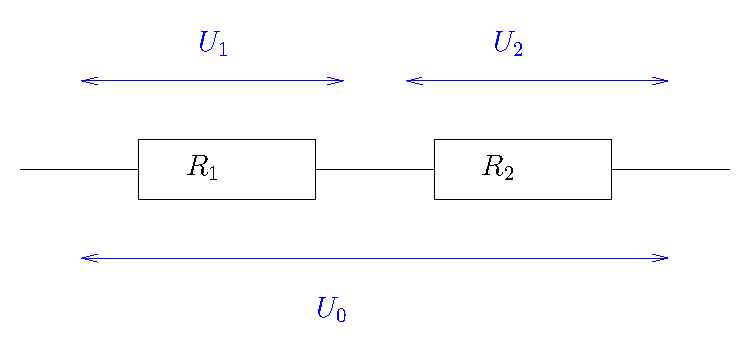
\includegraphics[height=0.235\textwidth]{bilder/reihe_strom}}
\hfill
\subfigure[Parallel]{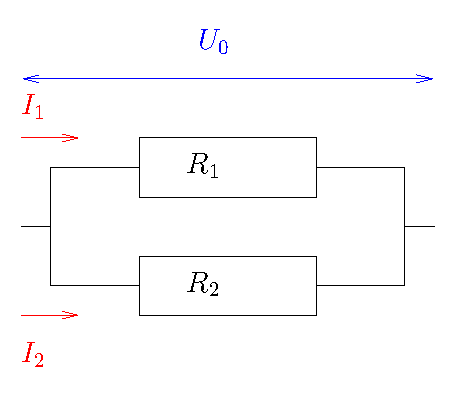
\includegraphics[height=0.235\textwidth]{bilder/parallel_strom}}
   \caption{Schaltung von Widerst"anden}
   \label{abb_schaltung_widerstaende}
\end{figure}












\subsection{Die \textsc{Kirchhoff}'schen Gesetze}
\label{kap_kirchhoffschen-gesetze}

Um diese Gesetze anwenden zu k"onnen, teilt man eine Schaltung
(bestehend aus \textbf{Knoten} und \textbf{Kanten}: Kanten sind Leiter
auf denen der Strom flie"st und Knoten sind die Punkte, an denen sich
Kanten treffen) in \textbf{\index{Maschen}Maschen} ein. Eine Masche
besteht aus einem geschlossenen Teil des Stromkreises; in ihm kann der
Strom auf genau einem Weg von einem Knoten im "`Kreis"' flie"sen,
dabei alle Knoten und Kanten der Masche durchflie"sen und schlie"slich
wieder zum Ausgangspunkt zur"uckkehren.

Man definiert nun in der Schaltung an jeder Kante eine
Stromrichtung: Diese ist nur entscheidend f"ur die Wahl der Vorzeichen
f"ur die eigentlichen \textbf{Kirchhoff}'schen Gesetze. Dazu zeichnet
man in einer Masche eine "`Wirbelrichtung"' (in willk"urlicher
Richtung) ein und bestimmt nach den folgenden Gesetzm"a"sigkeiten, wie
die Elemente der Kante verrechnet werden.



\begin{Wichtig}
   [\index{Knotenregel}Knotenregel]
Die Summe aller gerichteten Str"ome an einem Knoten verschwindet:
\begin{equation}
   \label{eq:170}
   \sum_i I_i \equiv 0
\end{equation}
\end{Wichtig}

"`Gerichtet"' bedeutet dabei, dass wenn der Strom in einen Knoten
hineinl"auft er ein anderes Vorzeichen hat, als wenn er herausl"auft.

Zu erkl"aren ist das ganz einfach dadurch, dass der Strom in der
Schaltung ja nicht verlohren gehen darf; Was an Strom in den Knoten
l"auft (oBdA positiv) muss auch wieder herausflie"sen (oBdA negativ).

F"ur Spannungen entsprechend:
\begin{Wichtig}
   [\index{Maschenregel}Maschenregel]
Die Summe aller gerichteten Spannungen in einer orientierten Masche
verschwindet:
\begin{equation}
   \label{eq:171}
   \sum_i U_i \equiv 0
\end{equation}
\end{Wichtig}

"`Orientiert"' bedeutet dabei, das die Masche eine feste
Umlaufrichtung (oBdD im Uhrzeigersinn) hat.
Eine Spannungsquelle deren Stromrichtung in die Richtung
("`Orientierung"') der Masche zeigt bekommt ein positives
Vorzeichen\footnote{und entsprechend wenn ihr Strom \emph{entgegen}
  der Stromrichtung zeigt ein negatives} und ein Verbraucher dessen
Stromrichtung mit der Richtung der Masche "ubereinstimmt entsprechen
ein negatives Vorzeichen\footnote{Und somit ein positives Vorzeichen,
  wenn der Strom entgegen der Orientierung der Masche flie"st.}.

\begin{Wichtig}
   Dabei ist wichtig, dass man wirklich \emph{alle} Maschen beachtet
   -- also dass man alle m"oglichen Wege von und zur Spannungsquelle
   durchprobiert; f"ur jeden Weg bekommt man eine eigene Gleichung.
\end{Wichtig}


\begin{Beispiel}
   \emph{\index{Kondensatorentladung}Kondensatorentladung}. Siehe f"ur
   den Aufbau Abb. \ref{abb_kondensatorentladung_schaltplan}. Sei $C$
   geladen, bei $t = 0$ werde $S$ geschlossen. Die Str"ome und
   Spannungen an Kondensatorn und Widerstand werden im Index mit $C$
   bzw. $R$ gekennzeichnet, der Leiter bzw. Schalter habe keinen
   Widerstand.

Wir haben also eine Masche  M und zwei Knoten K' und K''. F"ur die
Masche gilt mit $U_R = I_R \cdot R$ und $U_C = \frac{Q_C}{C}$:
\begin{equation}
   \label{eqn_differenz-c78}
   U_R + U_C = 0 = I_R \cdot R + \frac{Q_C}{C}
\end{equation}
Wegen der Knotenregel ist
\begin{equation}
   \label{eqn_differenz-c79}
   I_R - I_C = 0 \text{ und damit } I_R = I_C = I = \dot Q
\end{equation}
Betrachtet man K', so flie"st hier Strom von $R$ hinein, und strom von
$C$ heraus. Bei K'' dagegen flie"st Strom von $C$ hinein und bekommt
das positive Vorzeichen und Strom von $R$ flie"st heraus und bekommt
das negative Vorzeichen: Wir h"atten lediglich
Gl. \eqref{eqn_differenz-c79} mit $(-1)$ multipliziert.

Wir haben also mit den beiden Gleichungen eine Differenzialgleichung
1. Ordnung
\begin{equation}
   \label{eqn_differenz-c80}
   R \cdot \dot Q + \frac{1}{C} \cdot Q = 0
\end{equation}
die wir mit dem Ansatz (mit $\lambda = -\frac{1}{\tau}$)
\begin{equation*}
   Q = Q(t) = \hat Q \cdot \exp \left ( - \frac{t}{\tau} \right )
\end{equation*}
angehen, und erhalten durch Einsetzen ($\hat Q$ ist durch eine
Anfangsbedingung zu bestimmen!)
\begin{equation*}
   \tau = R \cdot C
\end{equation*}

F"ur Strom und Spannung ergibt sich
\begin{equation*}
   I(t) = \frac{\diff }{\diff t} Q(t) = - \frac{1}{R C} \cdot  \hat Q
   \cdot \exp \left ( - \frac{t}{RC} \right ) \text{ und } U(t) = R
   \cdot I(t)
\end{equation*}

Der Kondensator entl"ad sich also exponentiell.
\end{Beispiel}




\begin{figure}
   \centering
% %    \subfigure[Schaltplan\label{abb_kondensatorentladung_schaltplan}]{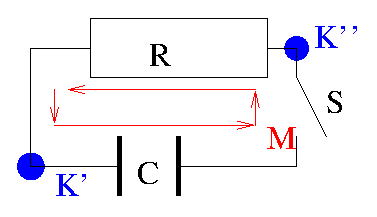
\includegraphics[width=0.35\textwidth]{bilder/RC}}
% \hfill
% \subfigure[Zeitlicher Verlauf: Auf der $y$-Achse ist $\hat U$, $\hat
% Q$ oder $\hat I$, auf der $x$-Achse Vielfache von $\tau$.]{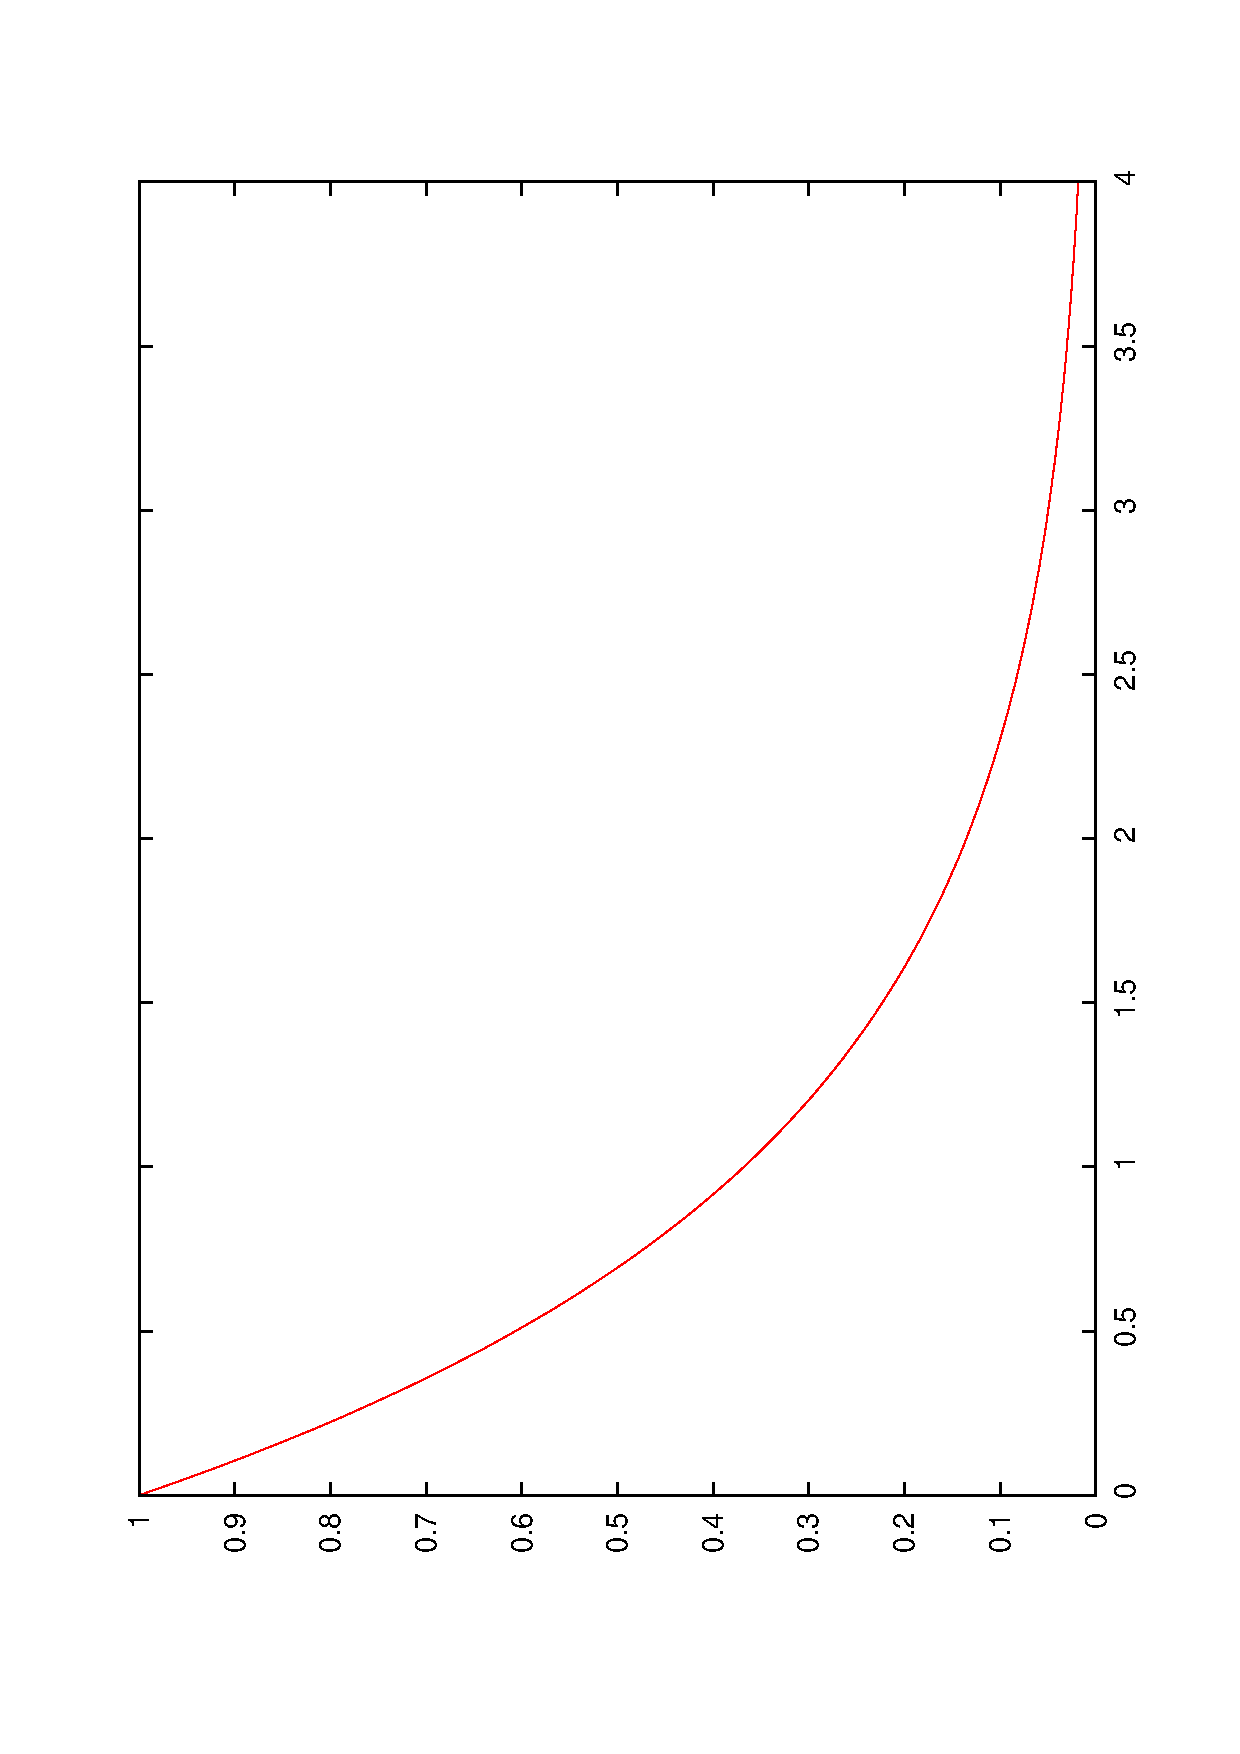
\includegraphics[angle=-90,width=0.6\textwidth]{bilder/spannung_RC}}
% %    \caption{Entladevorgang eines Kondensators}
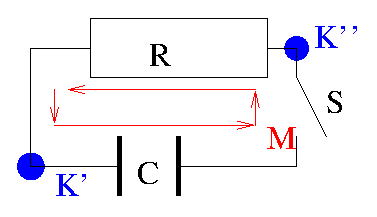
\includegraphics[width=0.35\textwidth]{bilder/RC}
\caption{Schaltplan
  RC-Glied}\label{abb_kondensatorentladung_schaltplan}
   \label{abb_kondensatorentladung}
\end{figure}










\subsection{Elektrische Arbeit und Leistung}
\label{kap_ekeltrische-arbeit-und-leistung}

Beim Stromfluss bewegen sich Ladungstr"ager $q$ von einem Ort hohen
Potentials $\varphi_1$ zu einen niedrigeren Potentials
$\varphi_2$. Dabei wird die Arbeit
\begin{equation}
   \label{eqn_differenz-c82}
   W = q \cdot \Delta \varphi = q \cdot U
\end{equation}
aufgewandt bzw. frei. Ist die Spannung $U$ zeitlich konstant, so
k"onnen wir bestimmen:
\begin{Def}
   [\index{Elektrische Leistung}Elektrische Leistung $P$] Leistung ist
   verrichtete Arbeit $\diff W$ je Zeitintervall $\diff t$. Bei
   konstanter Spannung gilt:
   \begin{equation}
      \label{eqn_differenz-c83}
      P = \frac{\diff W}{\diff t} =
\frac{\diff (q \cdot U)}{\diff t} =
\frac{\diff q \cdot U}{\diff t} =
\boxed{ I \cdot U = P}
   \end{equation}
\end{Def}
Und damit entsprechend auch
\begin{equation}
   \label{eqn_differenz-c81}
   W = \int_t P(\hat t) \diff \hat t \text{ und bei $P = \const$: } W = P \cdot t
\end{equation}

Bei einem \textsc{Ohm}'schen Widerstand ersetzt man mit $R = \frac{U}{I}$:
\begin{equation}
   \label{eqn_differenz-c84}
   P = \frac{1}{R} \cdot U^2 = R \cdot I^2
\end{equation}








\subsection{Gleichspannungserzeugung}
\label{kap_gleichspannungserzeugung}

Wenn wir eine Spannung nutzen wollen, m"ussen wir sie zuerst
\emph{erzeugen}. Egal, was f"ur ein Ger"at man daf"ur verwendet, so hat
dieses Ger"at einen elektrischen
\textbf{\index{Innenwiderstand}Innenwiderstand} $R_i$. Wenn das Ger"at
also die Spannung $U_0$ liefert (auch
"`\textbf{\index{elektromotorische Kraft}elektromotorische
  Kraft}"' oder "`\emph{\index{Klemmspannung}Klemmspannung}"'
genannt), so wird nicht die gesamte Spannung nutzbar. Vielmehr ist die
nutzbare Spannung $U$ abh"angig davon, wie gro"s der angelegte
(Au"sen)Widerstand $R$ (also der des Verbrauchers) ist: Der
Gesamtwiderstand des Systems\footnote{Modellhaft ist eine reale
  Spannungsquelle eine ideale Spannungsquelle, wobei an einem Ausgang
  der Widerstand $R_i$ angeh"angt ist; er ist zu dem angeschlossenen
  Verbraucher stets in Reihe.} ist dann $R_g = R_i + R$ und so flie"st
der Strom $I = \frac{U_0}{R_i + R}$.

Es f"allt also die Spannung $U_i = I \cdot R_i$ in der Spannungsquelle
an -- und diese ist f"ur den Verbraucher nicht nutzbar. Die nutzbare
Spannung $U$ ist also vielmehr
\begin{eqnarray}
\nonumber
   U &=&
 U_0 - I \cdot R_i
=
U_0 \cdot \left ( 1 - \frac{I \cdot  R_i}{U_0} \right )\\
\nonumber
&=&
U_0 \cdot \left ( 1 - \frac{ R_i}{R_g} \right )
=
U_0 \cdot \left ( 1 - \frac{ R_i}{R_i + R} \right )\\
   \label{eqn_differenz-c85}
&=&
\boxed{ U_0 \cdot  \frac{R}{R_i + R}  = U}
\end{eqnarray}
In Abb. \ref{abb_innenwiderstand} ist dies veranschaulicht. Man sieht
hier: Je kleiner der Innenwiderstand $R_i$ ist, desto unabh"angiger ist
die Nutzbare Spannung $U$ von der Gr"o"se des angelegten Widerstandes
$R$ -- und dies ist in der Technik nat"urlich angestrebt: Man will eine
Batterie, die immer 1.5V abgibt -- egal in welchem Verbraucher.

\begin{figure}
   \centering
   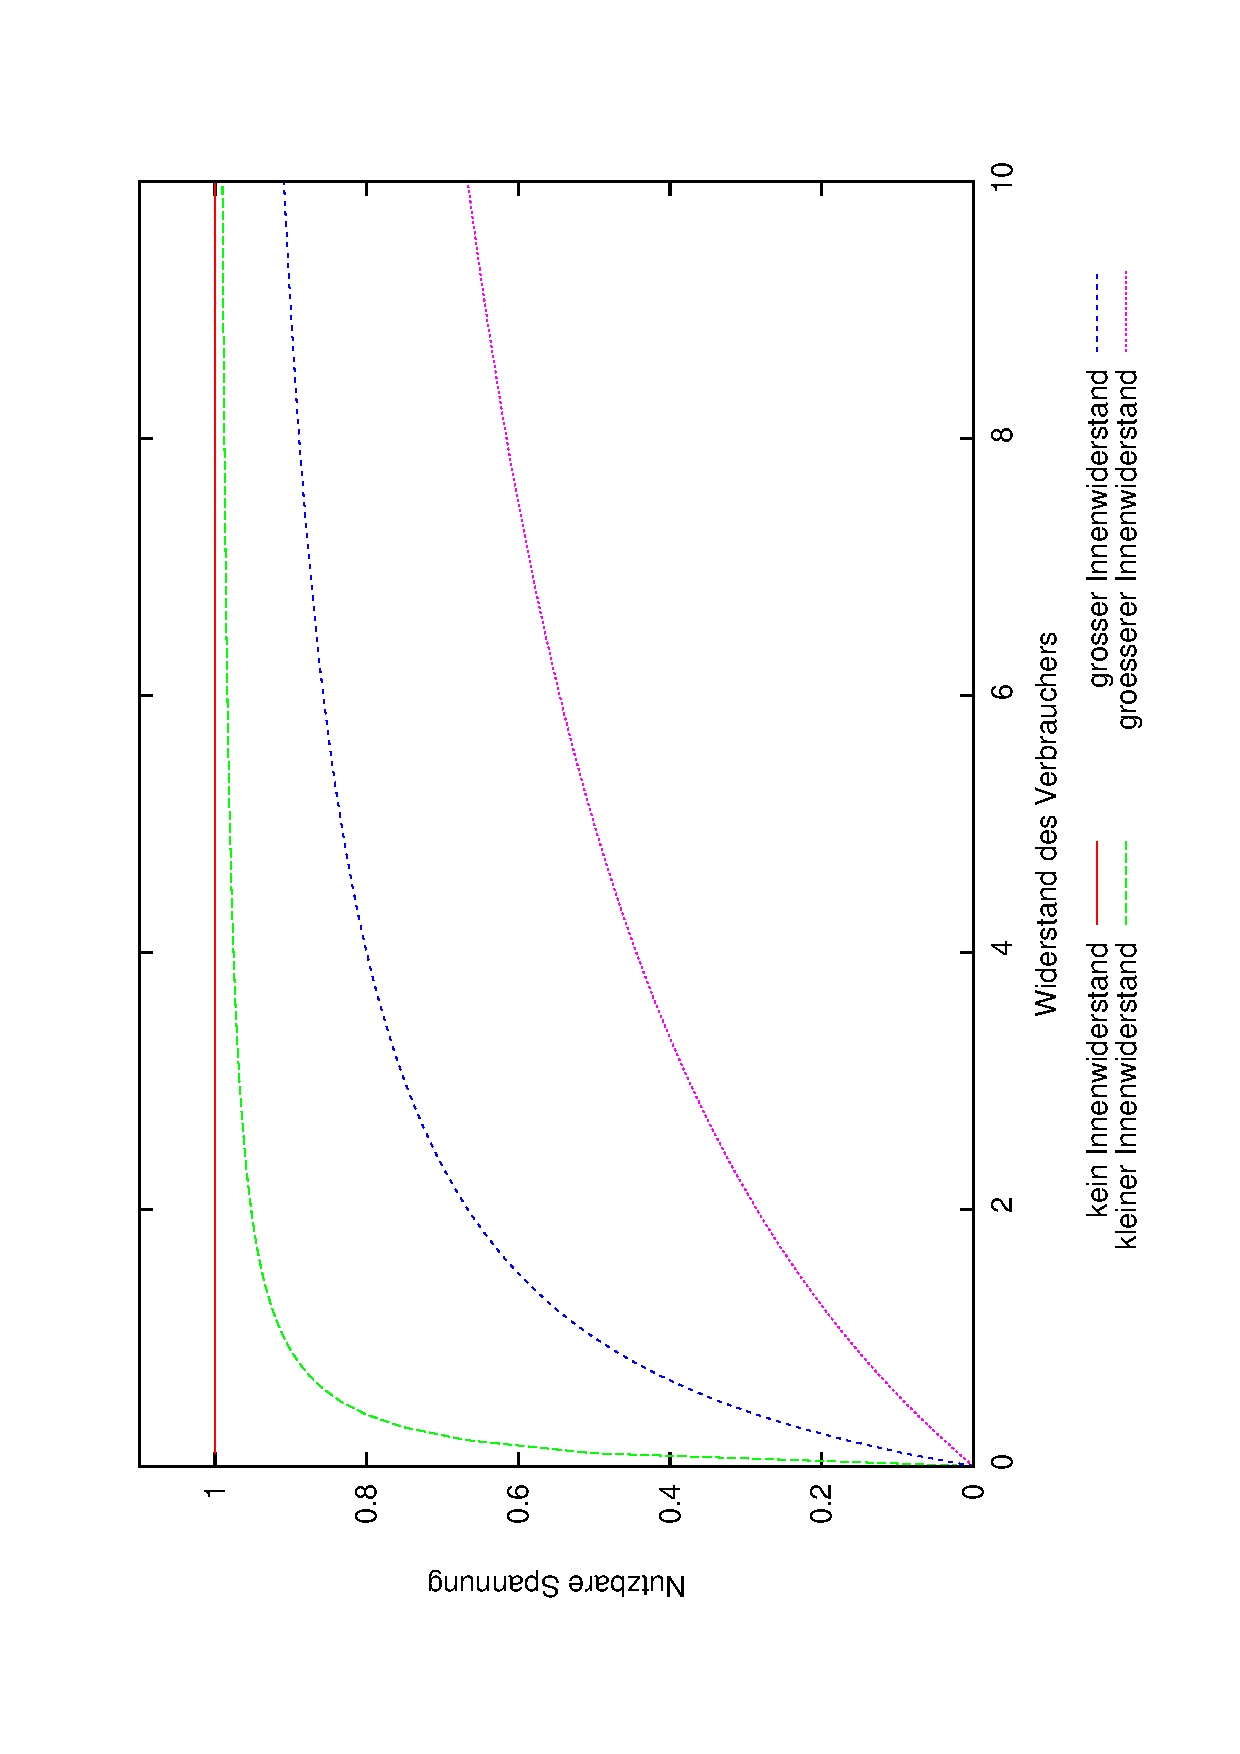
\includegraphics[angle=-90,width=\textwidth]{bilder/innenwiderstand}
   \caption{Nutzbare Spannung in Abh"angigkeit des Innenwiderstands}
   \label{abb_innenwiderstand}
\end{figure}





\begin{description}[\setlabelstyle{\bfseries\slshape}]
\item[\index{Galvanisches Element}\textsc{Galvani}sches Element] Gibt
   man ein Metall in L"osung, so haben die Metallatome Bestreben
   ("`\emph{\index{L"osungstension}L"osungstension}"' genannt) positiv
   ionisiert zu werden und in L"osung zu gehen. Dieses Bestreben h"angt
   vom Material ab (Bindungsenergie der Metallatome im Metall vs
   Ionisierungsenergie und Hydratationsenergie der Metallionen in
   L"osung).

   Das Metall wird durch die zur"uckbleibenden Elektronen negativ, die
   L"osung positiv. So ergibt sich ein E-Feld, welches die Positiven
   Ionen wieder in das Metallgitter zur"uckdr"uckt. Zwischen dem
   Bestreben des E-Felds und der L"osungstension stellt sich ein
   Gleichgewicht
   ein\footnote{\label{fn_bolzmann_loesungsgleichgewicht}Es handelt
     sich um ein \textbf{Boltzmann}-Gleichgewicht zwischen
     Konzentration im Metall ($c_M$) und Konzentration in der L"osunt
     ($c_L$), wobei das Potential der Teilchen im Metall $\varphi_M
     \cdot z \cdot e$ und in der L"osung $\varphi_L \cdot z \cdot e$
     ist. Es stellt sich dann ein Gleichgewicht ein ($U = \varphi_M -
     \varphi_L$): $$\frac{c_M}{c_L} = \exp \left ( - \frac{z \cdot e
          \cdot U}{K_B \cdot T} \right )$$}.

   Diese Anordnung wird ans \textbf{\index{Halbzelle}Halbzelle}
   bezeichnet. Um Strom flie"sen zu lassen, ben"otigt man noch eine
   zweite Halbzelle. Zwischen diesen beiden kann man eine
   materialcharakteristische Spannung $U$ messen.\footnote{Man kann
     die Spanung wirklich nur zwischen zwei Halbzellen messen, leider
     nicht die Spannung zwischen Metall und L"osung, weil man sonst in
     die L"osung ein Messinstrument tauchen m"usste, welches selbst die
     zweite Halbzelle bildet.} Die Spannung $U$ ergibt sich aus den
   Spannungen $U_g$ und $U_g'$, die zwischen Metall und L"osung
   bestehen, aber nicht gemessen werden k"onnen:
   $$U = U_g - U_g'$$
   Willk"urlich hat man festgelegt, dass eine platinierte Elektrode in
   einmolarer Salzs"aure die von Wasserstoffgas umsp"ult wird
   ("`\emph{\index{Standardwasserstoffelektrode}Standardwasserstoffelektrode}"'),
   das elektrochemische Potential $0$ bekommt. Misst man also die
   Spannung zwischen einer Halbzelle und dieser Standardzelle, so ist
   die gemessene Spannung die Spanung aus der \index{Elektrochemische
     Spannungsreihe} \emph{Elektrochemischen Spannungsreihe}. Je
   negativer hier die Spannungen, desto gr"o"ser die L"osungstension. Man
   sagt, das Metalle mit negativen Spannungen \emph{unedel} sind, die
   mit positiven Spannungen dagegen \emph{edel}.\index{Edle
     Metalle}\index{Unedle Metalle}

   Der Ladungstransport (Strom) ist hier mit Stofftransport verbunden:
   Am $\ominus$-Pol flie"sen die Elektronen ab, das r"ucktreibende
   Gegenfeld wird abgeschw"acht und mehr Metallatome gehen in
   L"osung. Die positiven Ionen werden durch ein E-Feld in der L"osung
   zum $\oplus$-Pol gezogen. Am $\oplus$-Pol kommen Elektronen an, das
   Gegenfeld wird verst"arkt und mehr Ionen kommen aus der L"osung als
   Atome ins Metall zur"uck.

   Wichtig ist, dass die L"osungen der beiden Halbzellen so verbunden
   sind, dass die Ionen wandern k"onnen, sonst baut sich in der L"osung
   ein unausgeglichenes E-Feld auf, welches den (eigentlich nutzbaren)
   Strom zum Erliegen bringt.

\item[\index{Membranspannung}Membranspannung] Seien zwei elektrisch
   neutrale L"osungen mit gro"sen negativen (bspw. $CL^-$) und kleien
   positiven (bspw. $K^+$) Ionen und stark unterschiedlichen
   Konzentrationen durch eine Membran getrennt. Die Membran habe
   Poren, die so klein sind, dass die kleinen Ionen
   hindurchdiffundieren k"onnen, die gro"sen jedoch nicht. Diese
   Diffussion geschieht durch \index{Osmose}osmotische Kr"afte: Die
   kleinen Ionen sind bestrebt, ihre Konzentration auf beiden Seiten
   der Membran gleich gro"s zu halten und diffundieren so an den Ort
   niedriger Konzentration. Die gro"sen Ionen k"onnen dies nicht tun. So
   werden die beiden L"osungen nicht mehr elektrisch neutral und es
   entsteht eine Spannung.\footnote{Analog zu Fu"snote
     \ref{fn_bolzmann_loesungsgleichgewicht} kann man hier die
     Spannung bestimmen:
     \begin{equation*}
        U = \frac{R \cdot T}{z \cdot \mathrm F} \cdot \ln \frac{c_1}{c_2}
     \end{equation*}
     mit der Molaren Gaskonstanten $R$, der \textsc{Faraday}'schen
     Konstanten $\mathrm F$ und der Ladung $z$.  }
\item[Kontaktspannung]\index{Kontaktspannung}
   Um ein Elektron aus einem Metall $M_1$ zu l"osen, braucht man Arbeit
   $W_1$, wenn es in ein anderes Metall aufgenommen wird, erh"alt es
   Arbeit $W_2$. Die Kontaktspannung ist dann
   \begin{equation}
      \label{eqn_differenz-c86}
      U_\text{Kontakt} = \frac{\Delta W_i}{e}
   \end{equation}

\item[Thermospannung] \index{Thermospannung} Man baut zwei gleiche
   Kontaktelemente hintereinander -- nur das eine in umgekehrter
   Reinehfolge, also $M_1$--$M_2$---$M_2$--$M_1$. Die Effekte durch
   die Kontaktspannung heben sich jetzt gerade wieder auf -- nicht
   aber, wenn man verschiedene Temperaturen anlegt: Die Abl"osearbeit
   ist Temperaturabh"angig. Die gemessene Spannung h"angt so also von
   der \emph{Temperaturdifferenz} an den beiden
   Kontaktspannungselementen ab.

   F"ur Kupfer gilt bspw. ein linearer Zusammenhang mit
   \begin{equation*}
      \label{eqn_differenz-c87}
      U_{Thermo} = 0.04 \frac{\operatorname{mV}}{\operatorname{K}} \cdot \Delta T
   \end{equation*}

   Auf diese Weise lassen sich Temperaturmessf"uhler sehr filigran
   ausf"uhren und sie nehmen Tempteratur"anderungen sehr schnell wahr.

\item[Peltierelement] Hier wird der Effekt der Thermospannung
   umgekehrt: Anstatt eine Spannung zu messen, legt man eien Spannung
   an und bekommt eine Temperaturdifferenz an den
   Kontaktspannungselementen: Die Elektronen bewegen sich st"andig "uber
   die Potentialdifferenzen und m"ussen einmal Energie abgeben (warm) und
   einmal aufnehmen (kalt).

\item[\index{Photospannung}Photospannung] Sto"sen ein positiv und ein
   negativ dozierter \emph{Halbleiter} zusammen, so bildet sich eien
   \emph{Raumladungszone} um die Kontaktstelle. Hier k"onnen
   einfallende Photonen absorbiert werden und Ladungstr"ager
   erzeugen. Durch das in der Raumladungszone herrschende E-Feld
   werden diese getrennt und Strom flie"st.

   Dies ist das Prinzip der Solarzelle.
\end{description}















\section{Das Magnetische Feld}




\subsection{Unterschied zum E-Feld, Erregung $(\bigstar)$}
\label{kap_unterschied-zum-e-feld-erregung}
\label{kap_magnetische-feld}

Statische Elektrische Felder werden von Ruhenden Ladungen
hervorgerufen, statische Magnetische Felder von ruhenden
Magneten. Interessan ist aber, dass in dem ruhenden Magneten der
eigentliche magnetische Effekt von bewegten Ladungen in den Atomen
selbst kommen.

Elektrische Felder werden von \emph{Monopolen} gebildet: Es ist
m"oglich, das eine einzelne positive oder negative Ladung alleine im
Raum liegt. Im Gegensatz dazu kann man einen Stabmagneten immer weiter
zerteilen und wird niemals einen \index{Magnetischer
  Monopol}magnetischen Monopol finden.\footnote{Das stimmt leider
  nicht mehr: In j"ungsten Forschungen sind die Effekte magnetischer
  Monopole nachgewiesen worden. Die Existenz von magnetischen
  Monopolen w"urde eine elegante Symmetrie zwischen B- und E-Feld
  ergeben. Bisher liegen die Monopole jedoch noch nicht
  \emph{isoliert} vor, sondern nur als \emph{Quasiteilchen} im Gitter
  eines exotischen Kristalls; einem \emph{\index{Spin-Eis}Spin-Eis}}
\begin{Wichtig}
   Ein Magnet besteht also immer aus Nord- und S"udpol, wobei sich
   gleichnamige Pole absto"sen und ungleichnamige anziehen.
\end{Wichtig}

Ein sehr bedeutender Unerschied zum Elektrischen Feld ist:
\begin{Wichtig}
   Feldlinien in Magnetfeldern sind immer geschlossen.
\end{Wichtig}
In Elektrischen Feldern gehen Feldlinien von einer positiven zu einer
negativen Ladung und enden dort. Bei einem Magneten laufen die
Feldlinien bei einem Pol los, laufen zum anderen Pol und laufen
\emph{innerhalb} des Magneten zur"uck.

\bigskip

In Analogie
zum Coulomb-Gesetz (vgl. Kap. \ref{kap_elektrische-ladung-und-})
definiert man als Entsprechung zur Ladung $Q$ die
\textbf{\index{Magnetische Polst"arke}Magnetische Polst"arke} $p$ und
findet so experimentell als Kraft zwischen zwei Magneten
\begin{equation}
   \label{eqn_differenz-c88}
   \vec F_{12} = \frac{\vec r_1  - \vec r_2}{\|\vec r_1 - \vec r_2\|} \cdot
   \frac{1}{4 \cdot \pi \cdot \mu_0} \cdot \frac{p_1 \cdot p_2}{\|\vec
   r_1 - \vec r_2\|^2}
\end{equation}
mit
\begin{Def}
   [\index{Magnetische
     Permeabilit"atskonstante}\index{Induktionskonstante}Magnetische
   Permeabilit"atskonstante $\mu_0$] oder "`Induktionskonstante"'
   \begin{equation}
      \label{eqn_differenz-c89}
      \mu_0 := 4\pi \cdot 10^{-7} \frac{\operatorname{V} \cdot \operatorname{s}}{\operatorname{A}\cdot\operatorname{m}}
   \end{equation}
\end{Def}

Diese Formel ist praktisch weniger Sinnvoll, weil es ja keine
Magnetischen Monopole $p_i$ gibt: N"ahrungsweise bekommt man dies aber,
indem man einen sehr langen Stabmagneten nimmt. So kann man
definieren:
\begin{Def}
   [\index{magnetische Erregung}magnetische Erregung $H$] eines
   Magneten der Polst"arke $p_1$ wird mithilfe eines Probemagneten  mit
   $p_2 \ll p_1$ definiert:
   \begin{equation}
      \label{eqn_differenz-c90}
      \vec H = \frac{\vec F}{p_2}
   \end{equation}
\end{Def}
Mit der Einheit $[H] = \frac{\operatorname{A}}{\operatorname{m}}$.

Eigentlich sollte man $\vec H$ als \textbf{magnetisch Feldst"arke} definieren --
es hat sich jedoch herausgestellt, dass man diesen Begriff f"ur die
Gr"o"se $\vec B$ mit
\begin{equation}
   \label{eqn_differenz-c91}
   \vec B = \mu_0 \cdot \mu_r \cdot \vec H
\end{equation}
reserviert mit der Einheit $[B] = T \text{ (Tesla) } =
\frac{\operatorname{V} \cdot
  \operatorname{s}}{\operatorname{m}^2}$. Betrachtet man das
Magnetische Feld als von bewegten Ladungen erzeugt, so findet man eine
bessere Analogie zum E-Feld im B-Feld, wobei man die Ladungsdichten
der Elektrostatik durch Stromdichten ($\to$ Bewegte Ladungen) ersetzt.
Aus Bequemlichkeit wird in diesem Script "`Magnetfeld"' und B-Feld
analog verwendet.

Doch sp"ater mehr dazu.






\subsection{Strom und Magnetfeld}
\label{kap_strom-und-magnetfeld}

Flie"st Strom durch einen Leiter, so erzeugt er kreisf"ormig darum ein
B-Feld.
\begin{Wichtig}
   Das Wirbel-B-Feld um einen stromdurchflossenen Leiter folgt der
   \index{Rechte-Faust-Regel}Rechten-Faust-Regel!
\end{Wichtig}
Zeigt der Daumen in die (technische) Stromrichtung, so bilden die
Finger der Hand die Richtung der B-Feldlinien.

\begin{Wichtig}
   Die St"arke des B-Feldes um einen Leiter, in dem der Strom $I$
   flie"st ist im Abstand $\vec r$ vom Leiter
   \begin{equation}
      \label{eqn_differenz-c92}
      \vec B(\vec r) = \frac{\mu_0}{2\pi} \cdot \frac{\vec I \times
        \vec r}{\|\vec r\|^2}
   \end{equation}
   wobei man die Stromst"arke als \emph{Pointing-Vector} verwendet.
\end{Wichtig}
Diese Formel findet sich \emph{experimentell}!

Um Abzusch"atzen, wie das B-Feld mehrerer trivialer Leiter
nebeneinander aussieht, bilden wir die B-Felder der einzelnen Leiter
und "uberlagern sie:
\begin{Wichtig}[\index{Superposition}Superposition]
   Es gilt das Superpositionsprinzip.
\end{Wichtig}
Ein paar der Erkenntnisse sind in Abb. \ref{abb_bfelder_leiter} dargestellt.


\begin{figure}
   \centering \subfigure[Einfacher
   Leiter]{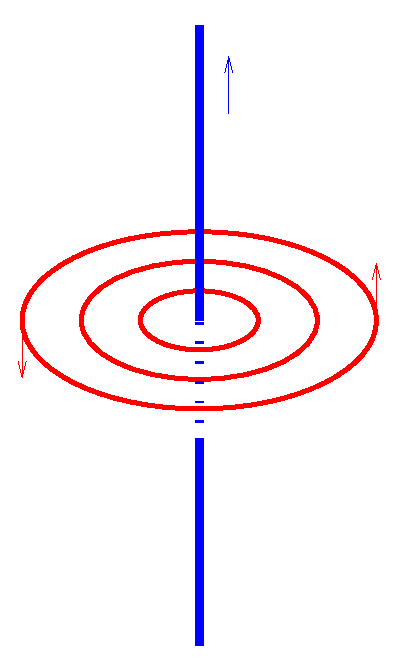
\includegraphics[height=0.2\textheight]{bilder/bfeld_leiter}}
   \subfigure[Leiterschlaufe]{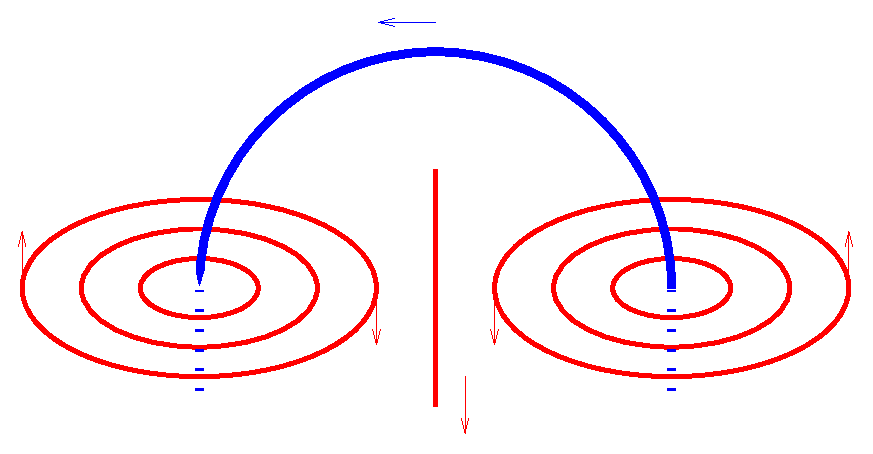
\includegraphics[height=0.13\textheight]{bilder/bfeld_schlaufe}}
    \subfigure[Parallele
    Leiter]{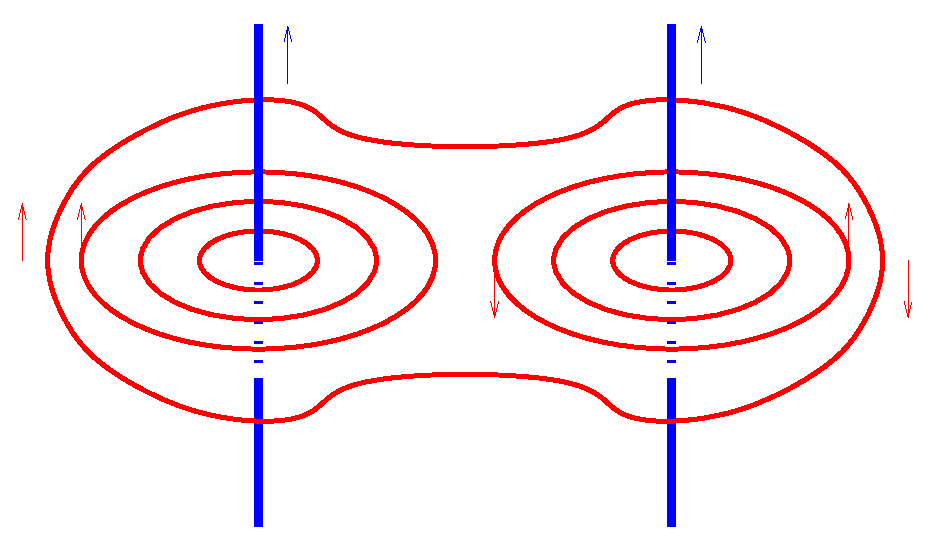
\includegraphics[height=0.11\textheight]{bilder/bfeld_parallel}}
\subfigure[Spule]{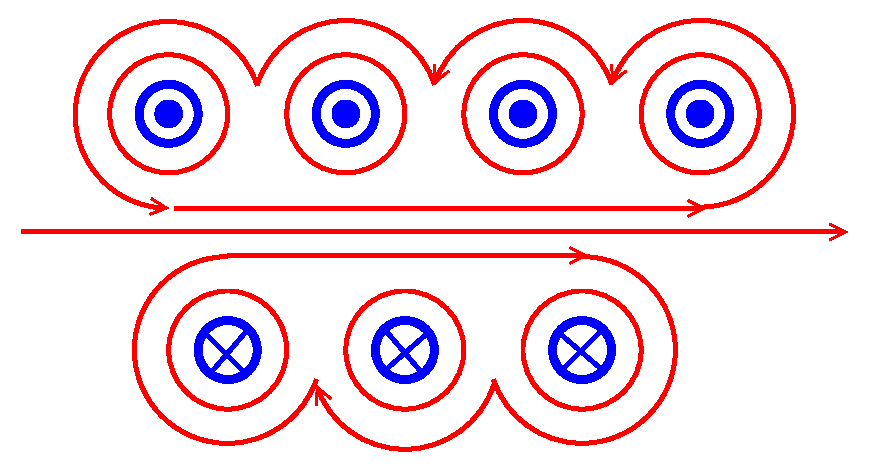
\includegraphics[height=0.11\textheight]{bilder/bfeld_spule}}
   \caption{B-Felder von Leitern}
   \label{abb_bfelder_leiter}
\end{figure}





\subsection{Das \textsc{Amp\`ere}'sche Gesetz}
\label{kap_ampersche-gesetz}

Analog zum Elektrischen Fluss $\Phi_E$ -- der auch
\emph{elektirscher Kraftfluss} hei"st -- definieren wir:
\begin{Def}
   [\index{Magnetischer Kraftfluss}\index{Magnetischer
     Fluss}Magnetischer (Kraft)Fluss $\Phi_B$] Die Anzahl an
   Magnetischen Feldlinien durch die Fl"ache $A$ ist:
   \begin{equation}
      \label{eqn_def_magn_kraftfluss}
      \Phi_B = \int_A \vec B \diff \vec A
   \end{equation}
\end{Def}
Mit der Einheit $[\Phi_B] = \text{T} \cdot \operatorname{m}^2 =
\operatorname{W} \text{ (Weber)}$.

Da alle Magnetfeldlinien geschlossen sind, bedeutet dies, dass in ein
Volumen $V$ genau so viele Feldlinien herein- wie herausflie"sen.
Integriert man also "uber die geschlossene Oberfl"ache eines Volumens
$V$ (also $A = \partial V$), ergibt sich
\begin{equation}
   \label{eqn_differenz-c94}
   \oint_A \vec B \diff \vec A = 0
\end{equation}
Mit dem Satz von \textsc{Gauss} (vgl. Kap. \ref{kap_satz-von-gauss})
finden wir (mit $A = \partial V$):
\begin{equation}
   \label{eqn_differenz-c93}
   \oint_A \vec B \diff \vec A = \int_V \vec \nabla \, \vec B \diff
    V = 0
\end{equation}
und damit
\begin{Wichtig}
   \begin{equation}
      \label{eqn_differenz-c95}
      \boxed{\vec \nabla \, \vec B = 0}
   \end{equation}
Die Divergenz des B-Felds verschwindet: Es hat also keine Quellen!
\end{Wichtig}


\abs
Wir wenden dies nun auf einen Stromdurchflossenen Leiter an und
integrieren das B-Feld einmal rund um den Leiter ($\gamma_1$)
$\oint_{\gamma_1}\vec B\diff \vec s$ und einmal
au"serhalb des Leiters mit zwei Strecken radial zum Leiter und zwei
kreissegmentigen ($\gamma_2$). Vlg. dazu
Abb. \ref{abb_amper_herleitung}.

Den Weg $\gamma_1$ kann man parametrisieren "uber
\begin{equation*}
   \vec r = R \cdot
   \begin{pmatrix}
      \sin \phi\\\cos\phi\\0
   \end{pmatrix} \text{ und } \phi \in [0;2\pi[
\end{equation*}
Weil wir uns im Kreis bewegen ist $\diff \vec s \parallel \vec B$ und damit
$\langle \vec B | \diff \vec s \rangle = \|\vec B\| \cdot \diff s$ und wegen
$\vec I \bot \vec r$ ist $\|\vec I \times \vec r\| = I \cdot r$ und Mit
Gl. \eqref{eqn_differenz-c92} gilt (Wir integrieren in Polarkoordinaten, also
$\diff s = r \diff \phi$):
\begin{equation}
   \label{eqn_differenz-c96}
   \oint_{\gamma_1} \frac{\mu_0}{2\pi} \frac{I}{\|r\|} \diff s =
   \oint_{\gamma_1} \frac{\mu_0}{2\pi} \frac{I}{R} r\diff \phi =
   \frac{\mu_0}{2\pi} \frac{I}{R}  \cdot \oint_{\gamma_1} r \diff \phi =
   \frac{\mu_0}{2\pi} \frac{I}{R} \cdot 2\pi R = \mu_0 \cdot I
\end{equation}
Integriert man stattdessen "uber $\gamma_2$, so gilt f"ur die
Parametrisierung $\phi \in [\alpha,\beta[$ ($\alpha$ und $\beta$ legen
den "Offnungswinkel des Segments fest). Hier tragen beiden radialen
Kanten nichts zum Integral bei, weil hier $\vec B \bot \diff \vec s$
ist und damit $\langle \vec B | \diff \vec s \rangle = 0$ ist, f"ur die
Kreissegmente ist die Argumentation wie oben.
 F"ur das Integral ergibt
sich:
\begin{equation}
   \label{eqn_differenz-c97}
   \oint_{\gamma_2} \frac{\mu_0}{2\pi} \frac{I}{\|\vec r\|} \diff s =
\frac{\mu_0}{2\pi} \cdot I \cdot   \int_0^{2\pi} \frac 1 {\|\vec
  r\|} r\diff \phi =
\frac{\mu_0 \cdot I}{2 \pi} \cdot \left (
[\frac{r_a}{r_a} \phi ]_\alpha^\beta + [\frac{r_b}{r_b} \phi
]^\alpha_\beta \right ) = 0
\end{equation}

Damit haben wir das gew"unschte Gesetz gefunden:
\begin{Wichtig}
   [\textsc{Amp\`ere}'sches Gesetz] F"ur einen beliebigen Weg $\gamma$
   gilt
   \begin{equation}
      \label{eqn_gesetz_ampere}
      \oint_\gamma \vec B \diff \vec s = \mu_0 \cdot I
   \end{equation}
wobei $I$ der von $\gamma$ eingeschlossene Strom ist.
\end{Wichtig}

\begin{figure}
   \centering
   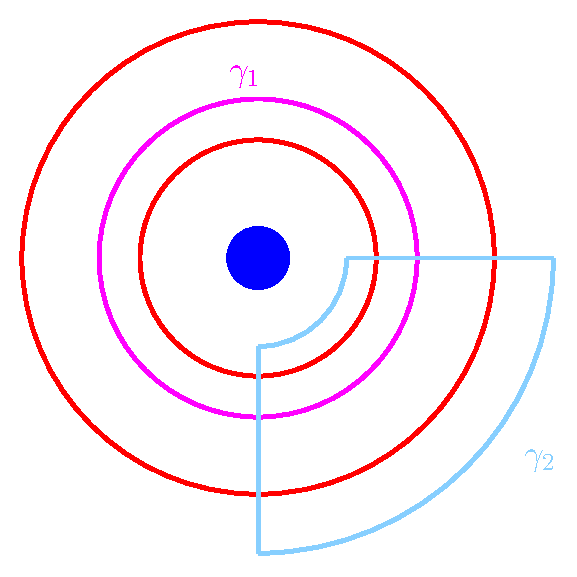
\includegraphics[width=0.3\textwidth]{bilder/amper-gesetz_int}
   \caption{Integrationswege zur Herleitung des \textsc{Amp\`ere}'schen Gesetzes}
   \label{abb_amper_herleitung}
\end{figure}


F"ur eine beliebige Stromverteilung $\vec j$ gilt nach Definition:
\begin{equation}
\label{eq:300}
   I = \int_A \vec j \diff \vec A
\end{equation}
Mit dem Satz von \textsc{Stokes} (vgl. Kap. \ref{kap_satz-von-stokes})
schreiben wir das Gesetz von \textsc{Amp\`er} um als
\begin{equation}
   \label{eqn_differenz-c99}
   \oint_\gamma \vec B \diff \vec s =  \int_A \vec \nabla \times \vec
   B \diff \vec A = \mu_0 \cdot I
\end{equation}
Und ein Koeffizientenvergleich mit Gl. \eqref{eq:300} lieftert:
\begin{Wichtig}
   \begin{equation}
      \label{eq:301}
\boxed{\vec \nabla \times \vec B = \mu_0 \cdot \vec j}
   \end{equation}
Das B-Feld ist ein Wirbelfeld, welches durch bewegte Ladungen
hervorgerufen wird.
\end{Wichtig}
In Integralschreibweise Lautet dies:
\begin{equation}
   \label{eq:302}
   \oint_\gamma \vec B \diff \vec s = \mu_0 \cdot \int_A \vec j \diff
   \vec A \text{ ~ ~ mit } \partial A = \gamma
\end{equation}





\subsection{B-Felder verschiedener K"orper}
\label{kap_b-felder-verschiedener-korper}


\subsubsection{Stromdurchflossener Leiter}
\label{kap_stromdurchflossener-leiter}


Wir betrachten zuerts einen {Stromdurchflossenen Leiter} mit
Durchmesser $2R$.  Wir
integrieren auf zwei konzentrischen kreisf"ormigen Wegen innen
$\gamma_i$ und au"sen $\gamma_a$.

Im Inneren nehmen wir Stromdichte $j$ als homogen und das B-Feld als
homogenes Wirbelfeld ($\vec B \parallel \vec s$ und damit $\langle
\vec B |\diff \vec s \rangle = B \cdot \diff s$) an. Dadurch
vereinfacht sich (mit dem Quotienten $\frac{r_1^2}{R^2}$ gibt man bei
einer Homogenen Stromdichte $j$ den Strom innerhalb eines Kreises mit
Radius $r_1$ an, wenn der gesamte Srom $I_0$ durch einen Kreis mit
Radius $R$ flie"st) das Wegintegral:
\begin{equation*}
   \label{eq:304}
   \oint_{\gamma_i} \vec B(\vec r) \diff s = \mu_0 \cdot \int_{A_i} \vec j
   \diff \vec A \text{ zu }
B(r) \cdot 2\pi r_1 = \mu_0 \cdot I_0 \cdot \frac{\pi r_1^2}{\pi R^2}
\end{equation*}
und damit\index{B-Feld!Leiter}
\begin{equation}
   \label{eq:305}
   B(r_1) = \frac{\mu_0 \cdot I_0 \cdot r_1}{2\pi \cdot R^2} ~\text{ mit
   } r_1 \in [0, R]
\end{equation}
\emph{Au"serhalb} des Leiters gilt analog (nur dass hier der Quotient
$\frac{r_1^2}{R^2}$ wegfallen kann, weil der eingeschlossene Strom sowieso $I_0$ ist):
\begin{equation}
   \label{eq:306}
   B(r_2) = \frac{ \mu_0 \cdot I_0}{2\pi \cdot r_2} ~\text{ mit } r_2
   \in [R, \infty[
\end{equation}
Das B-Feld steigt nach au"sen hin also linear bis zur Leiterh"ulle an
und f"allt dann reziprok proportional ab.

\subsubsection{Koaxialkabel}
\label{kap_koaxialkabel-1}



Analog ist beim {\index{Koaxialkabel}Koaxialkabel}, welches aus einem Innenleiter
mit Durchmesser $2R_i$ und einer Metallh"ulle mit Innenradius $2R_a$
(und vernachl"assigbarer Dicke) besteht das B-Feld:\index{B-Feld!Koaxkabel}
\begin{equation}
   \label{eq:307}
   B(r) =
   \begin{cases}
      \frac{\mu_0 \cdot I_0 \cdot r_1}{2\pi \cdot R^2}  & \text{ f"ur
   } r \in [0, R_i]\\
\frac{ \mu_0 \cdot I_0}{2\pi \cdot r_2}  & \text{ f"ur } r
   \in [R_i,R_a[\\
0 & \text{ f"ur } r \in [R_a, \infty[
   \end{cases}
\end{equation}
Au"serhalb der Metallh"ulle verschwindet das B-feld. Das liegt
daran, dass hier der Strom, der im Innenleiter hin flie"st, wieder
zur"uckkommt. Die Summe der eingeschlossenen Str"ome verschwindet damit
und mit dem Gesetz von \textsc{Amp\`ere} muss so auch das B-Feld
verschwinden.

\subsubsection{Lange, d"unne Spule}
\label{kap_lange-dunne-spule}



Bei einer {Langen Spule} betrachtet man einen Integrationspfad
$\gamma$, der um $N$ Windungen herumf"uhrt, parallel zur Spule die
L"ange $L$ hat und der entweder
parallel zu $\vec B$ oder senkrecht dazu ist -- wo $\diff s \| \vec B$
ist n"amlich wieder $\langle \vec B |\diff \vec s  \rangle  = B \cdot
\diff s$ und f"ur $\diff s \bot \vec B$ ist $\langle \vec B | \diff
\vec s  \rangle = 0$ und muss nicht ber"ucksichtigt werden.

Zudem ist in der Spule das B-Feld Innen weit gr"o"ser als Au"sen, und so
kann man $\vec B_\text{au"sen} \approx \vec 0$ setzen. Wir rechnen:
\begin{equation*}
   \label{eq:308}
   \oint_\gamma B \diff s = B \cdot L = \mu_0 \cdot N \cdot I
\end{equation*}

\begin{Wichtig}\index{B-Feld!Spule}
   F"ur eine \textbf{lange, d"unne Spule} (L"ange $L$, Windungszahl $N$) gilt
   \begin{equation}
      \label{eqn_B-spule}
      B = \frac{ \mu_0 \cdot N \cdot I}{L}
   \end{equation}
\end{Wichtig}
Es ist deshalb wichtig, dass die Spule lang und d"unn ist, weil wenn
$\gamma$ sich "uber die komplette L"ange $L$ erstreckt, wir am Ende der
Spule eigentlich nicht mehr den Integrationsweg senkrech zu $L$
ignorieren d"urfen, weil hier das Feld zur Seite geht und so eine
Komponente parallel zu $\diff \vec s$ hat. Bei einer langen d"unnen
Spule ist dieser Effekt vernachl"assigbar.

In der Technik wird oft die \textbf{Windungsdichte} $n = \frac{N}{L}$
angegeben; daf"ur gilt
\begin{equation*}
   B  = \mu_0 \cdot n \cdot I
\end{equation*}







\subsection{Das \textsc{Biot-Savart}'sche Gesetz}
\label{kap_bio-savartsche-gesetz}

Das \textsc{Amp\`ere}'sche Gesetz ist zwar allgemein anwendbar, aber
nicht immer einfach \emph{handhabbar}. Das Linienintegral ist bei
komplizierteren Leiterformen schwierig zu berechnen. Stattdessen
zerlegen wir den Leiter in kleine Volumenelemente der L"ange $\diff l$ (mit
Pointing-Vector $\diff \vec l$ in Richtung Stromfluss)
und bestimmen dann an einem Punkt $P$ (der Verbindungsvektor vom
Volumenelement zu $P$ ist $\vec r$) den Beitrag des Volumenelements
zum B-Feld.  Es gilt dann:
\begin{Wichtig}
   [\textbf{Biot-Savart}'sches Gesetz] \index{Biot-Savart'sches
     Gesetz} Am Punkt $P$ gilt f"ur den Beitrag des Volumenelements an
   der Stelle $P \text{~``+''} -\vec r$ zum B-Feld:
   \begin{equation}
      \label{eqn_biot-savart}
      \diff \vec B = \frac{\mu_0 \cdot I}{4 \pi \cdot r^3} \left (
         \diff \vec l \times \vec r \right )
   \end{equation}
\end{Wichtig}
"Uber die Anteile $\diff \vec B$ summiert oder integriert man.




\subsection{Das Vektorpotential $(\bigstar)$}
\label{kap_vektorpotential}

\begin{Wichtig}
Das B-Feld darf kein (skalares) Potential haben:
\end{Wichtig}
  (GA)\footnote{Beweis durch \textbf{G}egen\textbf{a}nnahme} Es existiere ein
B-Feld-Potential $\varphi_B$, dann ist $B = - \vec \nabla \varphi_B$
und f"ur die Rotation gilt\footnote{Der Beweis f"ur diese Identit"at
  l"asst setzt voraus, dass die partiellen Ableitungen nach $x^j$ und
  $x^k$ vertauschbar sind -- dies sei gegeben! Der Beweis geht elegant
mit dem $\varepsilon$-Tensor und \textsc{Einstein}-Notation:
$$
\left [ \nabla \times (\nabla \varphi)
\right ]^i
=
 \varepsilon^i_{jk} \frac{\partial }{\partial
  x^j}\frac{\partial }{\partial x^k}\varphi
=
\stackrel{\oplus}{\varepsilon}^i_{jk} \frac{\partial }{\partial
  x^j}\frac{\partial }{\partial x^k}\varphi + \underbrace{\stackrel{\ominus}{\varepsilon}^i_{jk} \frac{\partial }{\partial
  x^j}\frac{\partial }{\partial x^k}\varphi }_{
\stackrel{\oplus}{\varepsilon}^i_{kj} \frac{\partial }{\partial
  x^k}\frac{\partial }{\partial x^j}\varphi
}
=
0
$$
wobei $\stackrel{\oplus}{\varepsilon}$ nur die \emph{positiven}
F"alle von $\varepsilon$ abdeckt und $\stackrel{\ominus}{\varepsilon}$
entsprechend nur die \emph{negativen}.}
\begin{equation*}
   \vec \nabla \times \left ( \vec \nabla \, \varphi_B \right ) = 0
\end{equation*}
Dies ist aber nicht korrekt, sobald sich Ladungen bewegen
(vgl. \eqref{eq:301} und damit ein Widerspruch. q.e.d.

Weil aber andererseits $\vec \nabla \, B = 0$ (vgl. \eqref{eqn_differenz-c95})
ist, kann man eine Vektorgr"o"se $\vec \Apot$ definieren:
\begin{Def}
   [\index{Vektorpotential des B-Felds}Vektorpotential des B-Felds]
   Wir definieren $\vec \Apot$ so, dass
   \begin{equation}
      \label{eq:303}
      \vec B = \vec \nabla \times \vec \Apot ~ \text{ und } \vec
      \nabla \vec \Apot = 0
   \end{equation}
Die zweite Bedingung hei"st \textbf{\index{Coulomb-Eichung}Coulomb-Eichung}.
\end{Def}
Die Eichung ist n"otig, weil man sonst statt $\Apot$ auch $\Apot + \vec
\nabla \, \omega$ mit beliebiger Skalarfunktion $\omega$ h"atte
verwenden k"onnen:
\begin{equation*}
   \vec \nabla \times \left ( \Apot + \vec \nabla \, \omega \right )
=
   \vec \nabla \times \Apot  +    \underbrace{\vec \nabla \times \left ( \vec
      \nabla \, \omega \right)}_{\vec 0}
\end{equation*}


\bigskip

Wir wollen nun $\vec \Apot$ aus einer gegebenen Stromdichte $\vec j$
bestimmen. Dazu brauchen wir aus der Vektoranalysis (dies entspricht
der BAC-CAB-Regel!)
\begin{equation}
   \label{eqn_differenz-c98}
   \vec \nabla \times \left ( \vec \nabla \times \vec \Apot \right )=
\vec \nabla \cdot ( \vec \nabla \cdot \Apot ) -  \Laplace \vec \Apot
\end{equation}
mit dem \textsc{Laplace}-Operator $\Laplace = \vec \nabla \cdot \vec \nabla$. Wegen \eqref{eq:301}
und weil $\vec \nabla \, \vec \Apot = 0$ (nach Def.) wissen wir:
\begin{equation}
   \label{eq:309}
   \Laplace \vec \Apot = - \mu_0 \cdot \vec j
\end{equation}
Dies ist eine partielle Differenzialgleichung 2. Ordnung mit der
L"osung
\begin{equation}
   \label{eq:310}
   \vec \Apot(\vec r_1) = \frac{\mu_0}{4\pi} \int_{V_2} \frac{\vec
     j(\vec r_2)}{\|\vec r_1 - \vec r_2\|} \diff V_2
\end{equation}
Dabei betrachtet man $\vec \Apot$ am Punkt $\vec r_1$ und integriert
"uber das gesamte stromf"uhrende Volumen $V$: Hier (Punkt $\vec r_2$)
bestimmt man die Stromdichte im infinitissimalen Volumen $\diff V_2$.

Um nun das B-Feld zu bestimmen, wendet man $\vec \nabla_1 \times \cdot$ auf
Gl. \eqref{eq:310} an (die 1 im Index von $\nabla$ bedeutet, dass wir
nach den Koordinaten $\vec r_1$ ableiten -- integrieren jedoch nach
denen an $\vec r_2$). Weil die Stromdichte gen"ugend Gutartig ist,
darf man den Operator mit dem Integral vertauschen und erh"alt
\begin{equation}
   \label{eq:311}
   \vec B(\vec r_1) = \frac{\mu_0}{4\pi} \int_{V} \frac{\vec \nabla_1
     \times \vec
     j(\vec r_2)}{\|\vec r_1 - \vec r_2\|} \diff V_2
\end{equation}
Dies ergibt
\begin{equation}
   \label{eq:312}
     \vec B(\vec r_1) = \frac{\mu_0}{4\pi} \int_{V} \frac{\vec
     j(\vec r_2) \times \vec e_{12}}{r_{12}^2} \diff V_2
\end{equation}
Wobei $\vec r_{12} = \vec r_1 - \vec r_2$ ist und $\vec e_{12}$ der
Einheitsvektor in die Richtung.

Ist die Stromdichte homogen verteilt, kann man sogar noch weiter
vereinafachen: Weil $\diff V = \diff A \cdot \diff s$ ist
\begin{equation*}
   \vec j \diff V = \vec j \cdot \diff \vec A \cdot \diff \vec s = I \cdot
   \diff \vec s
\end{equation*}
und damit (das "`$-$"' kommt daher, weil das Kreuzprodukt gedreht wurde)
\begin{equation}
   \label{eq:313}
       \vec B(\vec r_1) = - \frac{\mu_0}{4\pi} \cdot I \cdot \int_{V}
       \frac{\vec e_{12} \times \diff \vec s}{r_{12}^2}
\end{equation}
Dies ist genau das \textsc{Bio-Savart}'sche Gesetz aus
Kap. \ref{kap_bio-savartsche-gesetz}.





\subsection{F"ormelchen}
\label{kap_formelchen}


Hier eine "Ubersicht "uber die bisher gefunden Gleichungen f"ur statische
B- und E-Felder:
\begin{center}
\begin{tabular}[c]{c l cl }
   \textbf{E-Feld} & ~ &\textbf{B-Feld} & ~ \\
   $\vec \nabla \times \vec E = \vec 0$ & wirbelfrei & $\vec \nabla \times \vec B =
   \mu_0 \cdot \vec j$ & durch bewegte Ladung erzeugt\\
   $\vec \nabla \, \vec E = \frac{\varrho}{\varepsilon_0}$ & Durch
   Ladung erzeugt & $\vec
   \nabla\,\vec B = 0$ & quellenfrei \\
   $\vec E = - \vec \nabla\,\varphi$ & hat (Skalar)Potential & $\vec B = \vec \nabla \times
   \vec \Apot$ & keine skalares- nur Vektorpotential\\
   \multicolumn{4}{c}{$\vec j = \sigma \cdot \vec E$ Die Verbindung (i)}\\
   \multicolumn{4}{c}{$c = \frac{1}{\sqrt{\varepsilon_0 \cdot \mu_0}}$
     Die Verbindung (ii)}
\end{tabular}
\end{center}









\section{Bewegung geladener Teilchen im B-Feld}
\label{kap_bewegung-geladener-teilchen-im-b}

Wir betrachten zeitlich konstante B-Felder:
 $$\dot{ \vec B } = 0$$




\subsection{Kraft auf ein Teilchen}
\label{kap_kraft-auf-ein-teilchen}

Experimentell ergibt sich, dass auf Teilchen der Ladung $q$, die sich
mit der Geschwindigkeit $\vec v$ in eienem B-Feld  mit dem Fluss $\vec
B$ bewegen, die Kraft $\vec F$ mit
\begin{equation}
   \label{eqn_kraft_in_bfeld}
\boxed{\vec F = q \cdot \left (\vec v \times \vec B \right )}
\end{equation}
wirkt. 
Wir nennen sie \textbf{\textsc{\index{Lorentzkraft}Lorentz}kraft}.

Interessant ist, dass die Experimente statt der Gleichheit eigentlich
nur eine \emph{Proportionalit"at} zeigen; Die explizite
\emph{Gleichheit} gilt nur, weil die Proportionalit"atskonstante in den
Einheiten "`verschwindet"'\footnote{Nur dank deren geschickter Wahl ist die
Proportionalit"atskonstante $1$.}.

\begin{Wichtig}
Die \textbf{allgemeine Lorentzkraft} wirkt auf ein Teilchen, welches
sich in einem B- und einem E-Feld bewegt:
\begin{equation}
   \label{eqn_kraft_in_E-B-Feld}
   \vec F = q \cdot \left ( \vec E + \vec v \times \vec B \right )
\end{equation}
\end{Wichtig}





\subsection{Magnetische Kraft auf einen Stromdurchflossenen Leiter}
\label{kap_magnetische-kraft-auf-einen-stromdurchflossenen}

Auf einen Leiter der \emph{effektiven} L"ange $L$ (also der die L"ange
$L$ \emph{senkrecht} zu dem B-Feldlinien hat) hat, und der vom Strom
$I$ durchflossen wird, wirkt eine Kraft: Der Strom besteht aus
bewegter Ladung ($n$ ist die Teilchen\emph{dichte} und $N$ die Teilchenzahl):
\begin{equation*}
   \label{eq:314}
   I = \frac{\diff }{\diff t} \left ( n \cdot A \cdot q \cdot L \right
   ) = n \cdot A \cdot q \cdot \underbrace{\dot L}_{\vec v_d}
\end{equation*}
und auf diese $N$ Teilchen wirkt die Lorentzkraft nach \eqref{eqn_kraft_in_bfeld}
\begin{equation*}
   \label{eq:316}
   \vec F = \underbrace{n \cdot \underbrace{A \cdot L}_V}_N \cdot q \cdot \left ( \vec v_d \times \vec B
      \right )
\end{equation*}
Setzt man hier das $\vec v_d$ von oben ein, gilt
\begin{equation}
   \label{eq:317}
   \vec F = L \cdot \left ( \vec I \times \vec B \right )
\end{equation}
Dabei macht man aus dem Strom $I$ einen \emph{Pointing-Vector}.


\bigskip

Man kann die Kraft auch in ihrer differenziellen Form schreiben. F"ur
ein Konstantes B-Feld gilt dann bei einer konstanten Bewegung $v$ der
Ladungen $q$:
\begin{equation*}
   \diff \vec F = \diff q (\vec v \times \vec B) = 
\diff q (\frac{\diff \vec s}{\diff t} \times \vec B) =
\frac{\diff q}{\diff t} (\diff \vec s \times \vec B) =
I \cdot (\diff \vec s \times \vec B)
\end{equation*}





\subsection{Der \textsc{Hall}-Effekt}
\label{kap_hall-effekt}

Flie"sen Elektronen durch einen Leiter, der von einem B-Feld durchsetzt
ist, so werden sie senkrecht zur Bewegugnsrichtung abgelenkt. In einem
normalen Stromleiter also an die Wand. Hier bildet sich ein negativer
Ladungs"uberschuss und Elektronen werden von hier abgesto"sen.

Irgendwann ist der Ladungs"uberschuss so gro"s, dass sich ein
Gleichgewicht zwischen Lorentzkraft und Coulombkraft bildet:
\begin{equation}
   \label{eqn_gg_EB}
   q \cdot (\vec v \times \vec B) = - q \cdot \vec E
\end{equation}

\begin{itemize}
\item Da $\vec B$ und $\vec E$ (durch Spannungsmessung: $E = \frac{U}{d}$)
bestimmbar sind, kann man $v$ bestimmen.
\item Wegen
\begin{equation*}
   \vec j = n \cdot \vec v \cdot q ~\text{ folgt } \vec v = \frac{
     \vec j}{n \cdot q}
\end{equation*}
und damit
\begin{equation}
   \label{eq:319}
   \frac{\vec j}{n \cdot q} \times \vec B = - \vec E
\end{equation}
kann man mit bekanntem $j$, $E$ und $B$ die Teilchendichte $n$
bestimmen -- und sogar das Vorzeichen von $q$: So kann man in Metallen
ermitteln, dass Elektronen Strom leiten und in Halbleitern (manchmal) L"ocher.
\item Ist $v = \const$ bekannt, so kann man daraus $B$ bestimmen
   (\textbf{\index{Hallsonde}Hallsonde}):
   \begin{equation}
      \label{eq:320}
      B_y = - \frac{E_z}{v}
   \end{equation}
\end{itemize}




\subsection{Bewegte Leiter im B-Feld}
\label{kap_bewegte-leiter-im-b-feld}

Bewegt man einen Leiter (L"ange $d$) durch ein B-Feld, so erfahren die
Ladungstr"ager darin eine Lorentzkraft, die f"ur positive und negative
Ladungstr"ager entgegengesetzt aber gleich stark ist: Die Summe der
Kr"afte hebt sich auf, es flie"st aber ein Srom.

Wenn der Leiter kein Teil eines Stromkreises ist, so bildet sich durch
die getrennten Ladungen ein E-Feld ("`Gegen-E-Feld"') $\vec E$. Im
Gleichgewicht gilt wieder \eqref{eqn_gg_EB}. Dieses E-Feld sorgt f"ur
eine \emph{Spannung} $U = {E} \cdot {d}$ im Leiter mit
\begin{equation*}
   U = - B \cdot v \cdot d
\end{equation*}

Wird der Leiter hin und her bewegt, so wird eine Wechselspannung
erzeugt: \textbf{\index{Generatorprinzip}Generatorprinzip}.




\subsection{Kraft auf einen magnetischen Dipol im B-Feld}
\label{kap_kraft-auf-einen-magnetischen-dipol}

\begin{Def}
   [\index{magnetisches Dipolmoment}magnetisches Dipolmoment $\vec
   \mdm$] (auch $\vec p_m$ oder $\vec m$) einer Leiterschleife der
   Fl"ache $A$, in dem Strom der St"arke $I$, flie"st, hat das
   Dipolmoment
   \begin{equation}
      \label{eq:315}
      \vec \mdm = I \cdot \vec A
   \end{equation}
\end{Def}
Wichtig ist dabei, dass das Dipolmoment \emph{senkrecht} zur
Leiterschlaufe steht!



\begin{figure}
   \centering
   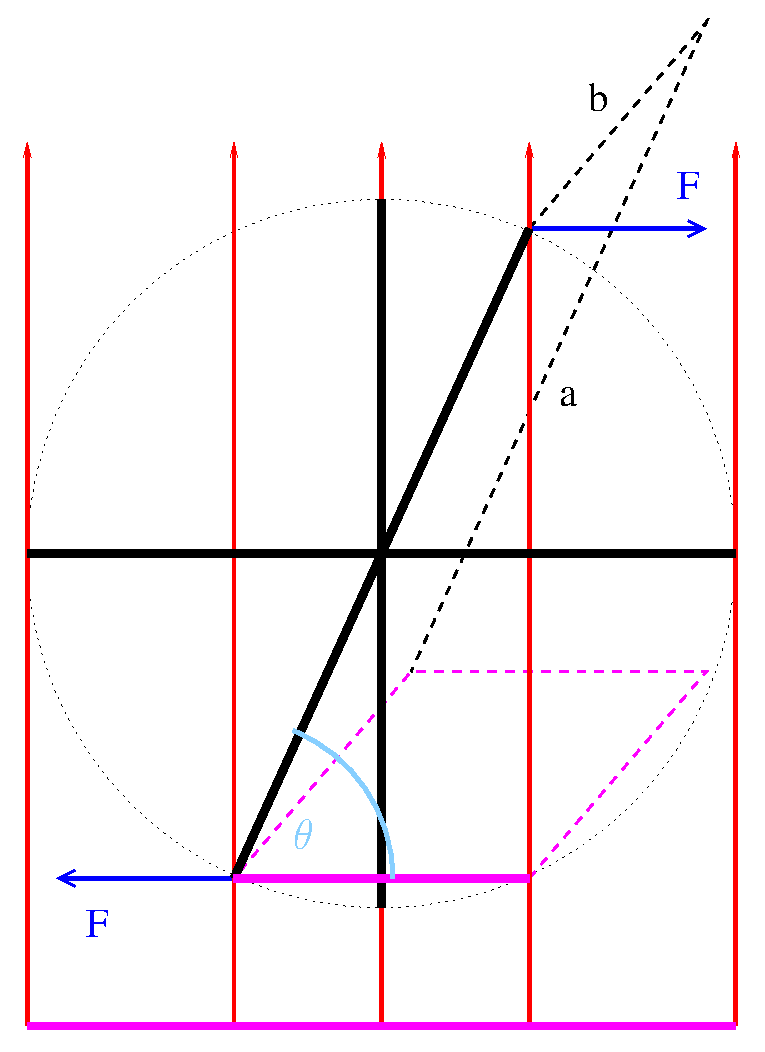
\includegraphics[width=0.5\textwidth]{bilder/schlaufe_bfeld}
   \caption[Schlaufe im B-Feld]{Schlaufe $A = a \cdot b$ im B-Feld mit
     Effektiver Fl"ache $A_e$ (pink) im Winkel $\theta$ geneigt}
   \label{abb_schlaufe-bfeld}
\end{figure}

Wir betrachten nun eine Leiterschlaufe der Fl"ache $A = a \cdot b$ im
B-Feld des Flusses $\vec B$.
(Vgl. Abb. \ref{abb_schlaufe-bfeld}). Die Elektronen, die an der
Vorderseite flie"sen haben eine Bewegungskomponente $\vec v^a_\bot$
senkrecht zu $\vec B$ und eine $\vec v^a_\|$ parallel zu $\vec B$. Nur
erstere ist f"ur eine Lorentzkraft verantwortlich\footnote{das
  $\times$-Produkt paralleler Vektoren verschwindet}. Da aber auf der
Vorderseite der Strom in die eine und auf der R"uckseite in die
Gegenrichtung flie"st, heben sich die entstehenden Kr"afte auf. Es ist
also nur die Bewegung der Elektronen auf der $b$-Kante interessant.

Mit Gl. \eqref{eq:317} folgt weil $\vec I_b \bot \vec B$:
\begin{equation}
   \label{eq:318}
   F = I \cdot B \cdot b
\end{equation}

Wir wollen nun das \emph{Drehmoment} $\vec M$ gem"a"s
Gl. \eqref{eqn_def_drehmoment} bestimmen, dazu l"osen wir das
Kreuzprodukt $\vec r\times \vec F$ auf zu
\begin{equation}
   \label{eq:321}
   M = 2 \cdot r \cdot F \cdot \sin \theta
\end{equation}
Die "`$2$"' kommt daher, dass die Kraft oben und unten
angreift. $\theta$ (bzw. sein Gegenwinkel) ist in
Abb. \ref{abb_schlaufe-bfeld} zu sehen.

Setzen wir \eqref{eq:318} und $2r = a$ ein, erhalten wir:
\begin{equation}
   \label{eq:322}
   M = a \cdot I \cdot B \cdot b \cdot \sin \theta
\end{equation}
Da $\theta$ auch der Winkel zwischen $\vec A = \vec e_A \cdot (ab) =
\vec a \times \vec b$ und $\vec B$ ist, k"onnen
wir dies schreiben als
\begin{equation}
   \label{eq:323}
   \vec M = I \cdot \vec A \times \vec B
\end{equation}
und weiter mit der Definition \eqref{eq:315}:
\begin{equation}
   \label{eq:324}
   \boxed{ \vec M = \vec \mdm \times \vec B }
\end{equation}

\bigskip

In Analogie zum E-Feld k"onnen wir folgern:
(Tab. \ref{tab_eigenschaften_dipol_bfeld})
\begin{table}[h]
   \centering
   \begin{tabular}{l c c }
\toprule
      ~&  \textbf{magnetischer Dipol} & \textbf{Elektrischer Dipol}\\
\midrule
Drehmoment $\vec M$ & $\vec \mdm \times \vec B$ & $\vec p \times \vec
E$\\
pot. Energie & $- (\vec \mdm \cdot \vec B)$ & $-(\vec p \cdot \vec E)$\\
Kraft $F$ (inhom. Feld) & $(\vec \mdm \cdot \vec \nabla)  \,  \vec B$ &
$(\vec p \cdot \vec \nabla) \, \vec E$\\
\bottomrule
   \end{tabular}
   \caption{Folgerungen aus Analogie zum E-Feld}
   \label{tab_eigenschaften_dipol_bfeld}
\end{table}



\begin{Beispiel}
\textbf{Exkurs}: Atomare magnetische Momente

In einem $H$-Atom kreist ein Elektron (Umlauffrequenz $\nu$) auf einer
Bahn (Radius $R$), was einem Wirbelstrom entspricht:
\begin{equation*}
   I = q \nu = q \frac{v}{2\pi R}
\end{equation*}
Wir bestimmen das Dipolmoment dieses Wirbelstroms (mit $v = \omega R$
und da $\vec A \| \vec \omega$ ist $\|\vec A\| = A = \pi R^2$):
\begin{equation*}
    \| \vec \mdm\| = q \nu \cdot A = q \frac{\omega}{2\pi} \pi R^2 =
    \frac{1}{2}q R^2 \, \omega \text{ bzw. } \vec \mdm =   \frac{1}{2}q R^2 \, \vec\omega
\end{equation*}

Der Drehimpuls des Elektrons ist
$$\vec L = m (\vec R \times \vec v ) = mR^2
\vec \omega$$
und ein Koeffizientenvergleich liefert einen Zusammenhang zwischen
Drehimpuls des Elektrons und magnetischem Dipolmoment:
\begin{equation}
   \label{eq:376}
   \vec \mdm = \frac{1}{2} \cdot \frac{q}{m} \cdot \vec L
\end{equation}


Da der Drehimpuls von Elektronen im $H$-Atom
\index{gequantelt}gequantelt ist und nur als ganzzahliges Vielfaches
$l \in \mathbb N$ vom \textsc{Planck}'schen Wirkungsquantum $\hbar$
vorkommt ($L = l \cdot \hbar$) k"onnen wir f"ur $l = 1$ einsetzen: $q
= -e$ und $m = m_e$.
\begin{equation}
   \label{eq:377}
   \mdm^e = \frac{1}{2} \frac{e}{m_e} \hbar =: \mu_B
\end{equation}
Diese Gr"o"se bezeichnet man als \textbf{\textsc{\index{Bohr'sches
      Magneton}Bohr}'sches Magneton}.
\end{Beispiel}








\subsection{Bahnen freier Ladungen im B-Feld}
\label{kap_bahnen-freier-ladungen-im-b}

Die Lorentzkraft steht senkrecht auf der Bewegungsrichtung und treibt
das Teilchen so in eine Kreisbahn; das Teilchen beh"alt seine
urspr"ungliche Geschwindigkeit bei, nur seine \emph{Richtung} wird
ver"andert, weil die Kraft keine bremsende ist, da sie nicht parallel
zur Geschwindigkeit wirkt: $\| \vec v \| = v_0$. Es gilt mit der
Zentripetalkraft:
\begin{equation}
   \label{eq:325}
   \frac{m \cdot v^2}{r} = q \cdot v \cdot B \text{ und damit } r =
   \frac{m v}{q B}
\end{equation}
Mit der Kreisfrequenz $\omega = \frac{v}{r}$ erzahlten wir die
\textbf{\index{Zyklotronfrequenz}Zyklotronfrequenz} $\omega_c$ zu
\begin{equation}
   \label{eq:326}
   \boxed{\omega_c = \frac{q}{m} \cdot B }
\end{equation}
Kreiselt also ein Teilchen in einem B-Feld, so h"angt seine
Kreisfrequenz nur von der St"arke des B-Felds und der
\textbf{spezifischen Teilchenladung} $\frac{q}{m}$ ab.


\begin{Beispiel}
\begin{description}[\setlabelstyle{\bfseries\slshape}]
\item[\index{Zyklotron}Zyklotron] (S. Abb. \ref{abb_zyklotron}) Ein
   Elektron wird zwischen metallenen Platten, die von einem B-Feld
   durchsetzt sind, durch eine angelegte Spannung $U$ beschleunigt (Es
   bildet sich ein E-Feld mit $E = \frac{U}{d}$). Innerhalb der
   Platten wird es ohne Geschwindigkeitsverlust abgelenkt und wieder
   zum Spalt zur"uckbef"ordert, wo es erneut beschleunigt
   wird, wof"ur die Polung der Platten nat"urlich umgekehrt werden muss.\footnote{Die Geschwindigkeit der Teilchen ist nach oben
     beschr"ankt, weil sie bei gro"sen Geschwindigkeiten Strahlen und so
     (Bewegungs)Energie verlieren.}
\item[\index{Massenspektrometer}Massenspektrometer] (S. Abb. \ref{abb_massenspektrometer})
   Teilchen einer Geschwindigkeit fallen in ein B-Feld ein und
   absolvieren je nach spezifischer Teilchenladung einen
   unterschiedlich gro"sen Radius. Ein Detektor registriert die
   Teilchenstr"ome.
\item[\index{Geschwindigkeitsfilter}Geschwindigkeitsfilter] (S. Abb. \ref{abb_geschwfilter}) Nur
   Teilchen, bei denen sich Lorentz- und Coulombkraft ausgleichen
   kommen durch die Blende: Sind sie zu schnell, werden sie vom B-Feld
   zu stark abgelenkt, sind sie zu langsam, sind sie zu lange im
   E-Feld und werden davon abgelenkt. Die Filtergeschwindigkeit ist:
   \begin{equation*}
      \label{eq:327}
      q \cdot \vec E = q \cdot (\vec v \times \vec B) \text{ oder } q
      E = q v B \Leftrightarrow E = Bv \Leftrightarrow v = \frac{E}{B}
   \end{equation*}
\item[\index{Schraubenbahn}Schraubenbahn] Ist $\vec v$ nicht senkrecht
   zu $\vec B$, so ist $\vec v = \vec v_\bot + \vec v_\|$ und damit
   \begin{equation}
      \label{eq:328}
      \vec F = q \cdot (\vec v \times \vec B)
= q \left ( (\vec
         v_\bot \times \vec B ) +  \underbrace{( \vec v_\| \times \vec
         B )}_{\vec 0}\right )
   \end{equation}
   Es ergibt sich also wegen $\vec v_\bot$ eine Kreisbewegung und
   $\vec v_\|$ wird davon nicht beeinflusst. Auf seiner Kreisbahn wird
   das Teilchen noch zus"atzlich in Richtung Kreisachse bewegt: Auf
   einer Schraubenbahn.
\item[\index{Teilchenfalle}Teilchenfalle]
   (S. Abb. \ref{abb_teilchenfalle}) Je tiefer das Teilchen kommt,
   desto st"arkter wird $\vec B$ und damit der Radius kleiner
   (Gl. \eqref{eq:325}). Weil das B-Feld inhomogen ist, hast die
   Lorentzkraft eine Komponente, die f"ur die Kreisbahn zust"andig ist,
   aber auch eine Komponente, die nach \emph{oben} zeigt: Das Teilchen
   wird abgebremst und schlie"slich nach oben reflektiert. Damit der
   Drehimpuls $L$ erhalten bleibt, rotiert das Teilchen schneller: Wegen
   \begin{equation*}
      L = m\omega r^2 = \const \text{ und mit } \omega =
      \frac{qB}{m} \text{ folgt } B \cdot r^2 = \const \text{ und } r
      \sim \frac{1}{\sqrt{B}}
   \end{equation*}
\end{description}
\end{Beispiel}


\begin{figure}
   \centering
   \subfigure[\label{abb_zyklotron}Zyklotron]{ 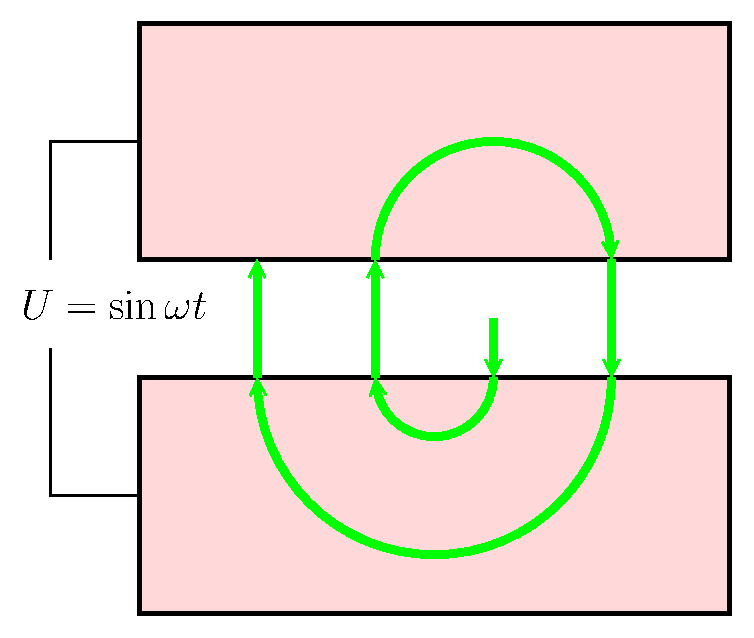
\includegraphics[width=0.23\textwidth]{bilder/zyklotron}}
\subfigure[Massenspektromet\label{abb_massenspektrometer}er]
{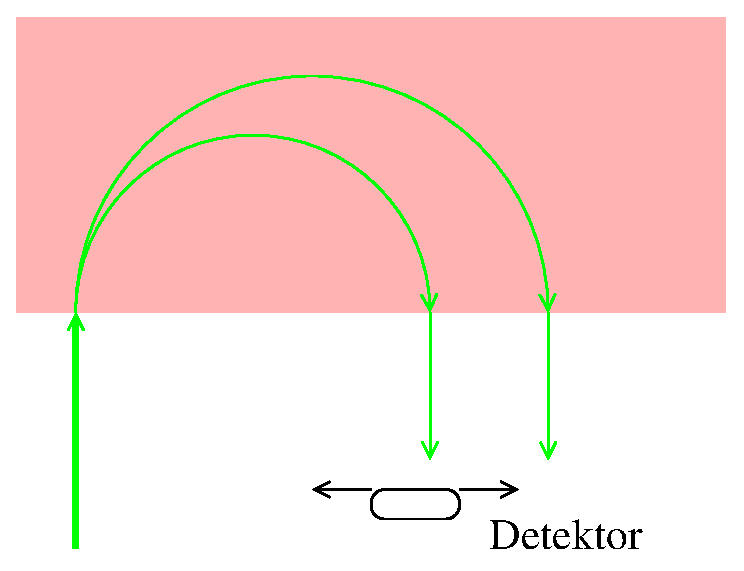
\includegraphics[width=0.2\textwidth]{bilder/massenspektrometer}}
\subfigure[Geschwindigkeitsfilte\label{abb_geschwfilter}r]{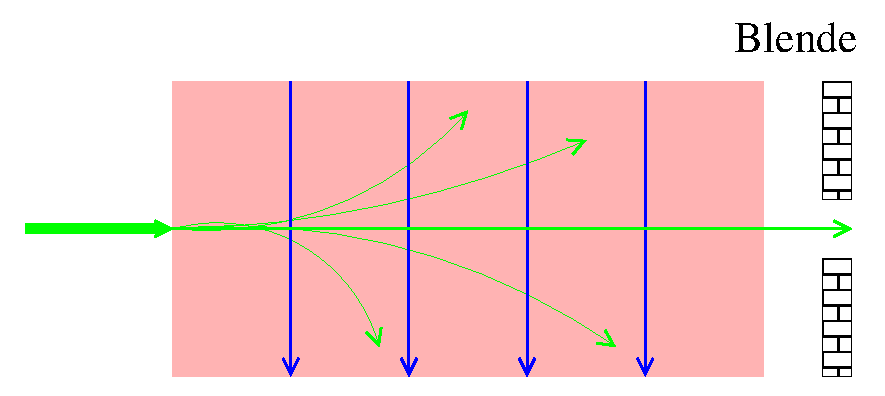
\includegraphics[width=0.28\textwidth]{bilder/geschwfilter}}
\subfigure[Teilchenfall\label{abb_teilchenfalle}e]{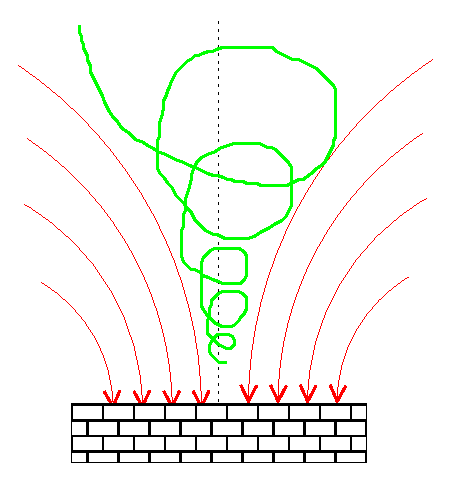
\includegraphics[width=0.25\textwidth]{bilder/teilchenfalle}}
\caption[Bahnen freier Ladungen im B-Feld]{Anwendung: Bahnen freier
  Ladungen im B-Feld}
   \label{abb_bahnen-im-bfled}
\end{figure}

















\section{Induktionserscheinungen}
\label{kap_induktionserscheinungen}




\subsection{\textsc{Faraday}'sches Induktionsgesetz}
\label{kap_faradaysches-induktionsgesetz}

Durch Experimente findet man:
\begin{Wichtig}
   [\textsc{\index{Faradaysches Induktionsgesetz}Faraday}'sches
   Induktionsgesetz]
"Andert sich der Magnetische (Kraft)Fluss durch eine Leiterschlaufe, so
wird die Spannung $U_i$ induziert:
\begin{equation}
   \label{eq:329}
   \boxed{U_i = - \dot \Phi_B} = - \frac{\diff }{\diff t} \int_A \vec B
   \diff \vec A
\end{equation}
\end{Wichtig}



\begin{Beispiel}
L"asst man eine Leiterschlaufe der Fl"ache $A$ in einem homogenen,
zeitlich konstanten B-Feld rotieren, wird Wechselstrom
induziert:\footnote{W"are $\vec B$ nicht homogen, so m"usste man f"ur
  $\Phi_B$ schreiben:
$$
\Phi_B(t) = \int_{A(t)} \vec B \diff \vec A ~ \text{ also bspw. } ~
\Phi_B(t) = \int_{\hat A \cdot \cos \omega t} \vec B \diff \vec A 
$$}
\begin{equation*}
   \label{eq:330}
   \Phi_B = \int_A \vec B \diff \vec A = \vec B \int_A \diff A = \vec
   B \cdot \vec A(t) = B \cdot \hat A \cdot \cos \theta
\end{equation*}
Ist $\theta$ der Winkel zwischen Spulennormaler ($\vec e_A$) und
B-Feldvektor, so gilt f"ur $\theta$, weil die Spule rotiert:
\begin{equation*}
   \theta = \omega t
\end{equation*}
Setzt man dies ein, folgt
\begin{equation*}
   \Phi_B = B \cdot \hat A \cdot \cos \omega t \text{ und } - \dot
   \Phi_B = - \left ( - B \cdot \hat A \cdot \omega \cdot \sin \omega t \right ) =U_i^{(1)}
\end{equation*}
F"ur $N$ Windungen gilt entsprechend
\begin{equation*}
   U_i^{(N)} = N \cdot B \hat A \omega \, \sin \omega t
\end{equation*}

\end{Beispiel}


Wenn man umgekehrt die Schlaufe festh"alt und das B-Feld variiert
($\vec B = \vec B(t)$), so ist
\begin{equation}
\label{eq:331}
   \Phi_B = \Phi_B(t) = \int_A \vec B(t) \diff \vec A \text{ und } - \dot \Phi_B = -
   \int_A \dot {\vec B}(t) \diff \vec A = U_i
\end{equation}
Diese Spannung kann auf ein E-Feld zur"uckgef"uhrt werden; mit
Gl. \eqref{eq:184} gilt:
\begin{equation}
   \label{eq:332}
   U = \int_\gamma \vec E \diff \vec s
\end{equation}
wobei $\gamma = \partial A$ ist. Demnach handelt es sich um einen
geschlossenen Integrationsweg -- also $\oint$ statt $\int$. Es gilt
mit dem Satz von \textsc{Stokes}
(vgl. Kap. \ref{kap_satz-von-stokes}):
\begin{equation}
   \label{eq:333}
  U = \oint_\gamma \vec E \diff \vec s = \int_A \vec \nabla \times \vec E
   \diff \vec A
\end{equation}
Ein Vergleich von Gl. \eqref{eq:331} und Gl. \eqref{eq:333} liefert:
\begin{Wichtig}
   \begin{equation}
      \label{eq:334}
      \vec \nabla \times \vec E = - \frac{\partial t}{\partial }{\vec
        B} = - \dot{\vec B}
   \end{equation}
   Eine zeitliche "Anderung des B-Felds induziert ein elektrisches
   \textbf{\index{Wirbelfeld}Wirbelfeld}!
\end{Wichtig}
Dieses induzierte E-Feld hat kein Potential: Es verl"auft rund um die
B-Feldlinien und beginnt und endet nicht bei Ladungen. Es verh"alt sich
also v"ollig anders, als wir es bisher kennengelernt hatten.

Das $\dot ~$ in Gl. \eqref{eq:334} steht f"ur eine \emph{partielle}
Zeitableitung. Diese abk"urzende Schreibweise sollte nur dann
verwendet werden, wenn eine Verwechslung mit der totalen Zeitableitung
ausgeschlossen ist!






\subsection{Die \textsc{Lenz}'sche Regel}
\label{kap_lenzsche-regel}

\begin{Wichtig}[\textsc{Lenz}'sche Regel]
\label{wichtig_lenzsche_regel}
   Die Induktion wirkt ihrer Ursache entgegen.
\end{Wichtig}

Verkleinert sich $\vec B$, so wird eine Spannung induziert welche
Ursache f"ur einen Strom ist, der wiederum
ein B-Feld hervorruft, welches $\vec B$ verst"arkt. Nimmt $\vec B$ zu,
so wirkt das neue B-Feld $\vec B$ entgegen.

\begin{quote}
   Werden in einem Leiter Str"ome induziert, so flie"sen diese so,
   dass sie die Bewegung, die sie verursachte, hemmen.
\end{quote}


\abs
Man kann dies mit dem Energieerhaltungssatz zeigen: Bewegt man einen
Magneten in eine Leiterschlaufe, so wird mit $U_i = - \dot \Phi_B$ ein
Strom $I = \frac{U_i}{R} = - \frac{\dot \Phi_B}{R}$ erzeugt. Dazu muss
in der Leiterschlaufe die Leistung $P = I^2 \cdot R$ aufgebracht
werden. Diese Leistung kommt aus der Kinetischen Energie des
Stabmagneten: Er wird gebremst, d.h. auf den Magneten wirkt effektiv
eine Kraft $\vec F$ entgegen $\vec v$. Diese Kraft Ist die Absto"sung
des Stabmagneten und dem B-Feld, welches sich durch den
Induktionsstrom etablieren konnte.

\abs
\begin{Beispiel}
Wir wollen ein paar Beispiele betrachten:
   \begin{itemize}
   \item Kurzzeitig hohe B-Felder erzeugen
      (S. Abb. \ref{abb_hohes_bfeld}): (Permantente Felder sind bis
      maximal 25T m"oglich.) Durch Sprengstoff wird die Fl"ache
      kurzfristig stark verkleinert; $\Phi_B$ "andert sich hier sehr
      stark : $\dot \Phi_B \ll 0$ und $U_i \gg 0$. Diese starke
      Spannung l"asst eine starken Strom flie"sen, welcher ein B-Feld
      induziert. Das induzierte Feld ist bis zu $1\, 400
      \operatorname{T}$ stark.
   \item Eine Leiterschlaufe aus einem B-Feld ziehen
      (S. Abb. \ref{abb_schlaufe_aus_bfeld}): Bewegt man die Schlaufe,
      wird ein Strom induziert. Die geladenen Teilchen erfahren eine
      Lorentzkraft entgegen der Zugrichtung.

      Ist der Widerstand $R \to 0$, so ist $I \to \infty$ und wegen $I
      \sim F$ ist der Leiter nicht zu bewegen. Bei $R \to \infty$
      dagegen geht $I\to 0$ und so auch $F \to 0$.

      W"ahlt man $R$ so, dass man das erzeugte B-Feld ignorieren kann,
      so ist
      \begin{equation*}
         \Phi_B = B \cdot b \cdot x  \text{ und } \dot \Phi_B = B
         \cdot b \cdot v \text{ und so } I = -\frac{B  b }{R} \cdot v
      \end{equation*}
      und damit die Lorentzkraft
      \begin{equation*}
         F = I \cdot B \cdot b = - \frac{B^2 \, b^2 }{R}\cdot v \sim - v
      \end{equation*}

Auf eine Spule "ubertragen hei"st das: M"ochte man eine Spule in ein
B-Feld einbringen, wird sie abgesto"sen: Der Fluss in der Spule soll
erh"oht werden und durch Induktion ensteht ein (absto"sendes)
Gegenfeld. M"ochte man sie herausziehen,
wird sie zur"uckbehalten: Der Fluss soll erniedrigt werden und durch
Induktion wird er erh"oht und das entstehende Feld verst"arkt das bestehende.

   \end{itemize}
   \begin{figure}[h]
      \centering
      \subfigure[\label{abb_hohes_bfeld}Hohes B-Feld
      erzeugen]{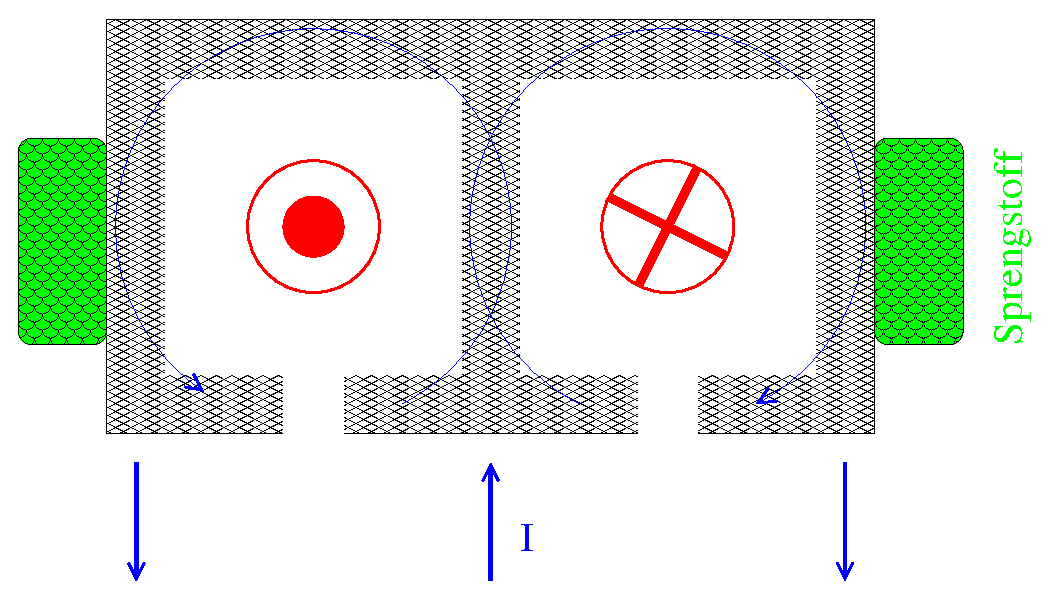
\includegraphics[width=0.4\textwidth]{bilder/hohes_bfeld}}
\subfigure[\label{abb_schlaufe_aus_bfeld}Schlaufe wird aus B-Feld gezogen]{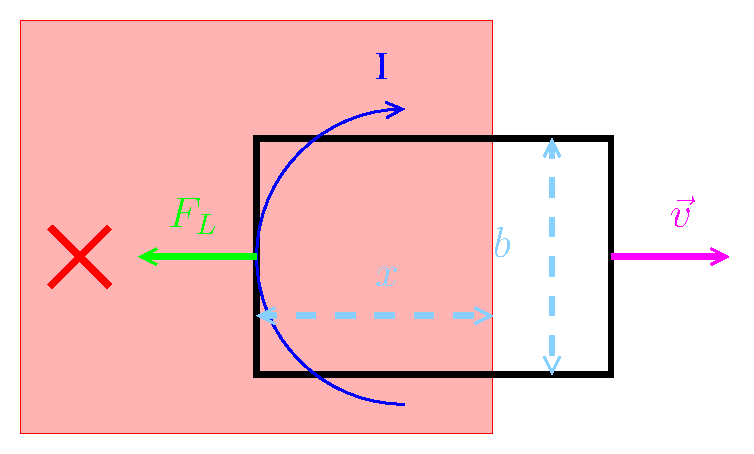
\includegraphics[width=0.4\textwidth]{bilder/schlaufe_bfeldF}}
      \caption{Beispiele f"ur das Induktionsgesetz}
      \label{abb_induktionsgesetz_bsp}
   \end{figure}
\end{Beispiel}






\subsection{Selbstinduktion}
\label{kap_selbstinduktion}

Eine Stromdurchflossene Leiterschleife baut ein B-Feld auf. Dieses
B-Feld selbst induziert eine Spannung in der Spule und "andert $U$
damit selbst.

Aus Kap. \ref{kap_b-felder-verschiedener-korper} wissen, ist in einer
Spule $B \sim I$ und damit innerhalb der Spule auch
\begin{equation*}
   \Phi_B \sim I \sim B
\end{equation*}
Die Proportionalit"atskonstante f"ur $\Phi_B \sim I$ hei"st
\begin{Def}
   [(\index{Eigeninduktivit"at}Eigen- oder \index{Selbstinduktivit"at}Selbst)\index{Induktivit"at}Induktivit"at
  $L$] ist der Quotient
  \begin{equation}
     \label{eq:335}
     L = \frac{\Phi_B}{I} \text{ oder differenziell } L = \frac{\diff
       \Phi_B}{\diff I}
  \end{equation}
\end{Def}
Mit der Einheit $[L] =
\frac{\operatorname{V}\cdot\operatorname{s}}{\operatorname{A}} = H
\text{ (Henry)}$.

Mit ihr lassen sich Induktionsspannungen $U_i$ einfacher berechnen,
als wenn man immer $\Phi_B$ und dann $\dot \Phi_B$ bestimmen muss. Es
gilt der wichtige Zusammenhang:
\begin{equation}
   \label{eq:336}
   \boxed{ U_i = -  L \cdot \frac{\diff }{\diff t} I } = - L \cdot
   \dot I
\end{equation}
"Andert sich in einer Spule also der Stromfluss, so wird eine Spannung
induziert, die dieser "anderung entgegenwirkt! Dieses Prozess hei"st
\textbf{\index{Selbstinduktion}Selbstinduktion}.

\bigskip
Wir bestimmen die Eigeninduktivit"at einer \textsc{Spule} der L"ange $l$
mit $N$ Windungen: Aus
\eqref{eqn_B-spule} wissen wir $B = \mu_0 I \frac{N}{l}$. Weil $\vec
B$ in der Spule (ann"ahrend) homogen ist, gilt
\begin{equation*}
   \label{eq:337}
   \Phi_B = B \cdot A = \mu_0 I \frac{N}{l} \cdot A \text{ und }
   -\dot\Phi_B = -\mu_0 \cdot \dot I \cdot \frac{N}{l} \cdot A = -\mu_0
   \frac{N}{l}A \cdot \dot I
\end{equation*}
und f"ur die Induktionsspannung
\begin{equation*}
\label{eq:338}
   U_i = -N \cdot \dot\Phi_B = -\mu_0
   \frac{N^2}{l}A \cdot \dot I
\end{equation*}
\begin{Wichtig}
   Die Induktivit"at $L$ einer langen d"unnen Spule ist
   \begin{equation}
      \label{eqn_induktivitaet_lange_Spule}
      L_{\text{Spule}} = \mu_0 \cdot \frac{N^2}{l}\cdot A
   \end{equation}
\end{Wichtig}
oder in technischerer Schreibweise
\begin{equation*}
   L_\text{Spule} = \mu_0 \cdot n^2 \cdot A \cdot l = \mu_0 \cdot n^2
   \cdot V
\end{equation*}



\begin{Beispiel}
   Ladevorg"ange bei einer Spule.
   \begin{figure}
      \centering
      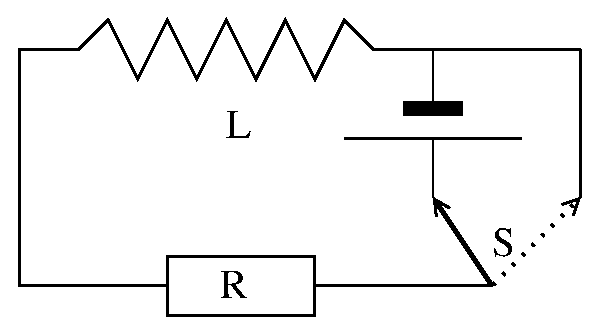
\includegraphics[width=0.3\textwidth]{bilder/laden_spule_schalt}
      \caption{Schaltplan beim Laden und Entladen einer Spule}
      \label{abb_spule_laden_schaltplan}
   \end{figure}
   Beim \textbf{Ausschaltvorgang} wird der Schalter $S$ ge"offnet. Aus
   der \emph{Maschenregel} folgt:
\begin{equation*}
   R I +  L \dot I = 0 \text{ oder } RI = -L\dot I
\end{equation*}
Dabei \emph{addiert} man bei der linken Gleichung, obwohl man nach der
Maschenregel ja eigentlich alle Spannungen aufsummiert; danach m"usste
gelten $RI + (-L \dot I) = 0$. Hier ist aber wichtig, dass die
Induktionsspannung $U_i = -L\dot I$ \emph{entgegen} der herrschenden
Spannung wirkt, deswegen m"ussen wir sie abziehen: $RI -(-L\dot I) =
0$. 

Die Spannung, $U_L$, die an der Spule selbst von au"sen anliegt
(so wie eine Spannung bspw. am Kondensator anliegt) ist
formal \emph{verschieden} von $U_I$: Dieses $U_i$ ist eine
(indirekte)\footnote{Aus der angelegten Spannung folgt ein Stromfluss
  und aus der "Anderung dieses Flusses folgt die Induktionsspannung.}
Folgerung aus der anliegenden Spannung $U_L$.


Die L"osung der DGL ist:
\begin{equation*}
   \label{eq:339}
   I(t) = \hat I \cdot \exp \left ( -\frac{ R}{L} \cdot t \right ) \text{
     also } \tau = \frac{L}{R}
\end{equation*}
Vergleiche dazu den Kondensator (Kap.
\ref{kap_kirchhoffschen-gesetze}): Hier war $\tau = R \cdot C$.

Mit der Anfangsbedingung $I(t = 0) = I_0$ folgt
\begin{equation}
   \label{eq:342}
   I(t) = I_0 \cdot\exp \left ( -\frac{ R}{L} \cdot t \right )
\end{equation}

F"ur den \textbf{Einschaltvorgang} gilt entsprechend mit der
Maschenregel
\begin{equation*}
   RI + L\dot I = U_0
\end{equation*}
Mit einem Ansatz vom Typ der Rechten Seite kann man dies L"osen:
\begin{equation*}
   I(t) = \hat I \cdot \exp \left (- \frac{ R}{L} \cdot t \right ) + I_0
\end{equation*}
Mit der Anfangsbedingung $I(t = 0) = 0$ folgt
\begin{equation*}
   I_0 = \frac{U_0}{R} \text{ und } \hat I = - I_0
\end{equation*}
und damit als L"osung
\begin{equation}
   \label{eq:340}
   I(t) = \frac{U_0}{R} \cdot \left (1 -  \exp \left (- \frac{ R}{L} \cdot t
   \right ) \right )
\end{equation}
\end{Beispiel}

\begin{Wichtig}
Induktionsspannungen werden nach der \textsc{Lenz}'schen Regel bei
Rechnung mit den \textsc{Krichhoff}'schen Gesetzen mit $(-1)$
multipliziert, weil sie der (eigentlichen) Spannung \emph{entgegen}wirken.
\end{Wichtig}






\subsection{Die Energie des B-Felds}
\label{kap_energie-des-b-felds}



Schaltet man eine Spule ab, so flie"st ein Strom
(s. Gl. \eqref{eq:342}). Dieser verrichtet am Widerstand\footnote{Man
  kann die Arbeit auch ohne Widerstand herleiten; der Ansatz ist der
  selbe: $W = \int P \diff t$, wobei diesmal $P = I \, L\dot I$
  ist. Integriert man dies nach $t$ so erh"alt man, weil $\dot I$ die
  "`innere Ableitung"' von $I$ ist: $W = \frac{1}{2}LI^2$.} die Arbeit
$W$ mit
\begin{eqnarray}
\nonumber
   W &=& \int_0^\infty I \cdot U \diff t = \int_0^\infty R I^2 \diff t
   \\
\nonumber
   &=& \int_0^\infty R \cdot I_0^2 \cdot \exp \left ( -\frac{2 R}{L}
      \cdot t \right ) \diff t 
= \left [ -I_0^2 \cdot \frac{L}{2} \cdot \exp \left ( -\frac{2 R}{L}
      \cdot t \right ) \right ]_0^\infty\\
\label{eq:343}
&=&\boxed{ \frac{1}{2} \cdot I_0^2 \cdot L = W}
\end{eqnarray}


Um die \textbf{\index{Energiedichte einer Spule}Energiedichte der
  Spule} zu bestimmen, setzen wir $L$ aus
Gl. \eqref{eqn_induktivitaet_lange_Spule} und $B$ aus
Gl. \eqref{eqn_B-spule} ein:
\begin{equation*}
   \label{eq:341}
   \varrho_{E,V} = \frac{W}{V} = \frac{1}{2} \mu_0 A l
     \left(\frac{N}{L}\right)^2 \cdot I_0^2 \cdot \frac{1}{V} =
   \frac{1}{2} \cdot Al \cdot \frac{1}{V} \cdot \frac{1}{\mu_0} \cdot B^2
\end{equation*}
und erhalten so
\begin{equation}
   \label{eq:344}
   \varrho_{E,V} = \frac{1}{2} \cdot \frac{1}{\mu_0} \cdot B^2
\end{equation}




\bigskip
Diese Formeln sind wieder denen des E-Feldes sehr "ahnlich:
\begin{tabular}[c]{c c}
   \textbf{E-Feld} & \textbf{B-Feld} \\
$W = \frac{1}{2} C U^2$ & $ W = \frac{1}{2} L I^2$\\
$\varrho_{E,V} = \frac{1}{2} \varepsilon_0 E^2$ & $\varrho_{E,V} =
\frac{1}{2} \frac{1}{\mu_0} B^2$
\end{tabular}















\section{Wechselstromkreis}
\label{kap_wechselstromkreis}

Bei einem Stromkreis mit einem \textbf{\textsc{Ohm}'schen Widerstand}
schwingen Strom und Spannung in Phase. Statt der (Momentan)Leistung $P
= P(t)$ verwendet man
\begin{Def}
   [\index{Wirkleistung}Wirkleistung $\bar P$] Dies ist der Mittelwert
   der Leistung:
   \begin{equation}
      \label{eq:345}
      \bar P = \frac{1}{T} \cdot \int_0^T P(t) \diff t
   \end{equation}
\end{Def}
Im Wechselstrom mit $U(t) = \hat U \cos \omega t$ ist
\begin{equation}
   \label{eq:346}
   \bar P = \frac{1}{2\pi} \cdot \int_0^{2\pi} {\hat I} \cdot \hat U \cos^2
   \theta \diff \theta = \frac{1}{2} \cdot \hat U \cdot \hat I
\end{equation}

W"urden wir statt des Wechselstroms Gleichstrom verwenden, sodass sich die
selbe Wirkleistung ergibt, w"urde man
\begin{equation}
   \label{eq:347}
   U_e(t) = \frac{1}{\sqrt{2}} \hat U \text{ und }    I_e(t) = \frac{1}{\sqrt{2}} \hat I
\end{equation}
verwenden. Dies bezeichnet man auch als
\begin{Def}
   [\index{Effektiver Strom}Effektiver Strom $I_e$
   bzw. \index{Effektive Spannung}Effektive Spannung $U_e$]
   Gleichstrom, der die selbe Leistung abgibt, wie der entsprechende
   Wechselstrom:
$$\bar P_e \equiv \bar P$$
\end{Def}
Man schreibt f"ur das (zeitliche) Mittel einer Gr"o"se $x$ manchmal auch
$\langle x \rangle$.

\bigskip

Verf"ugt der Stromkreis dagegen "uber eine \textbf{Spule} oder einen
\textsc{Kondensator}, so sind Strom und Spannung nicht mehr in
Phase. Sei bspw.
\begin{equation*}
   U = \hat U \cdot \cos \omega t \text{ und } I = \hat I \cdot \cos
   (\omega t + \varphi)
\end{equation*}
wobei $\varphi$ die (zeitlich konstante) \emph{Phasenverschiebung} angibt, so ist die
Wirkleistung abh"angig von derselben:\footnote{Zur Integration
  ben"otigt man das Additionstheorem (\textsc{Bronstein}\textsuperscript{7} Gl (2.124))
  $\cos a \cdot \cos b = \frac{1}{2} \left ( \cos(a-b) + cos(a+b)
  \right )$ und kann anschlie"send $x = 2\theta + \varphi$
  substituieren.}
\begin{equation*}
   \bar P = \frac{1}{2\pi} \int_0^{2\pi} U I \diff \theta =
   \frac{1}{2\pi} \hat U \hat I \cdot \int_0^{2\pi} \cos\theta \cdot
   \cos(\theta + \varphi) \diff \theta = \frac{1}{2} \hat U \hat I
   \cdot \cos \varphi
\end{equation*}


\bigskip Um dreiphasige Wechselspannung zu erzeugen, l"asst man einen
Magneten rotieren und h"alt drei Spule in der N"ahe in denen die
Spannung induziert wird
(\textbf{\index{Generatorprinzip}Generatorprinzip}). Die drei Spulen
werden symmetrisch um den rotierenden Magneten verteilt und alle an
einem Ende geerdet. So erh"alt man drei Phasen, die alle um
$\frac{2\pi}{3}$ phasenverschoben sind:
\begin{equation*}
   \label{eq:348}
   U_1 = \hat U \cos(\omega t + 0) \text{ , ~ }
   U_2 = \hat U \cos(\omega t + \frac{2\pi}{3}) \text{ und ~ }
   U_3 = \hat U \cos(\omega t + \frac{4\pi}{3})
\end{equation*}
Verwendet man nun eine der Phasen gegen die Erde, erh"alt man
"`normale"' Wechselspannung mit $\hat U$. Schaltet man dagegen zwei
Phasen gegeneinander, so erh"alt man\footnote{Additionstheorem $\cos a
  - \cos b = -2 \sin \frac{a + b}{2} \cdot \sin \frac{a-b}{2}$,
  \textsc{Bronstein}\textsuperscript{7} Gl. (2.118)}
\begin{equation*}
    U_1 - U_2  = -2 \hat U \cdot \sin (\omega t + \frac{\pi}{3}) \cdot \sin
   \frac{2\pi}{3}  = - \sqrt{3} \cdot \hat U \cdot \sin (\omega t + \Delta \varphi)
\end{equation*}

Man kann auch weitere Spulen hinzuf"ugen und bekommt so mehrphasigen Strom.











\subsection{Komplexe Widerst"ande}
\label{kap_komplexe-widerstande}

Wir betrachten einen Stromkreis, der nur eine Spule $L$
(\textbf{\index{Induktivit"at}Induktivit"at}) und eine
Wechselspannungsquelle enth"alt. Nach der Maschenregel
(vgl. \ref{kap_kirchhoffschen-gesetze}) gilt, wenn die Spannung $U =
\hat U \cos \omega t$ angelegt wird:\footnote{Interessant ist hier,
  dass die Induktivit"at positiv auf der Seite der Spannungsquelle
  steht. Diest ist aber nur folgerichtig, weil wir oben
  (Kap. \ref{kap_selbstinduktion}) besprochen hatten, dass $U_i$ der
  allgemeinen Stromrichtung \emph{entgegen}l"auft und damit eigentlich
ein "`$-$"' verdient. Wir h"atten also rein formal aufgestellt: $-U -
U_i = 0$ (das Minus bei $U$, weil hier eine \emph{Quelle} ist).}
\begin{equation}
   \label{eq:349}
   U + U_i = 0 \text{ bzw } \hat U \cos \omega t = L \dot I \text{ und
   damit } \dot I = \frac{\hat U}{L} \cos \omega t
\end{equation}
L"ost man dies per Integration nach $t$, erh"alt man
\begin{equation}
   \label{eq:350}
   I = \frac{\hat U}{\omega \cdot L} \sin \omega t = \hat I \cdot \sin
   \omega t \text{~ mit } \hat I = \frac{\hat U}{\omega \cdot L}
\end{equation}
Damit hat man eine \emph{Phasenverschiebung} zwischen Strom $I$ und
Spannung $U$ von $\varphi = \frac{\pi}{2}$: \emph{Der Strom flie"st der
Spannung um $90^\circ$ hinterher.} Zuerst muss eine Spanung aufgebaut
werden, damit Strom flie"sen kann.

Der \textbf{induktive Widerstand} der Spule ist im reellen
\begin{equation}
   \label{eq:351}
   |R_\text{Spule}| = \frac{\hat U}{\hat I} = \omega \cdot L
\end{equation}






\abs
\begin{quote}
Wir f"uhren nun einen Formalismus ein; wir betrachten \textbf{Strom und
Spannung} in der \textbf{Komplex}en Ebene:
\begin{equation*}
   \label{eq:352}
   Z, U, I \in \mathbb C
%\text{ ~ bspw. }  I(t) = \hat I \cdot \e^{\omega t + \varphi}
\end{equation*}
Die eigentlich messbaren Gr"o"sen stellen den \emph{Realteil} der Zahl
dar, w"ahrend der \emph{Imagin"arteil} als Blindwert bezeichnet
wird. D.h. der Strom flie"st zwar im Stromkreis, kann dort jedoch keine
Arbeit verrichten.\footnote{Dass diese eigentlich nicht messbaren
  Blindwerte existieren sieht man bei gro"sen Firmen: Diese m"ussen f"ur
  (gro"se) Blindwerte bezahlen, weil diese daf"ur sorgen, dass die
  Leistung kurzzeitig aus dem Netz gezogen werden und sofort danach
  wieder eingespeist werden: Das belastet das Stromnetz.}
\end{quote}






\abs
Wir wollen nun die Rechnung zur Spule nochmal im Komplexen
durchf"uhren. Die Gr"o"sen, mit denen wir oben gerechnet haben seien die
jeweilgen Realteile:\footnote{Achtung: $U \in \mathbb C$ aber $\hat U
  \in \mathbb R$!}
\begin{equation}
   \label{eq:353}
   U = \hat U \E^{\I \omega t} = \hat U \left ( \cos \omega t +  \I \cdot
       \sin \omega t \right ) \text{ also } \Re U = \hat U \cos \omega t
\end{equation}
Analog zu Gl. \eqref{eq:349} gilt:
\begin{equation}
   \label{eq:354}
   \dot I = \frac{\hat U}{L} \E^{\I \omega t}
\end{equation}
und damit mit Integration
\begin{equation}
   \label{eq:355}
   I = \frac{\hat U}{\I \cdot \omega \cdot L} \cdot \E ^{\I \omega t}
\end{equation}
Mit $\I = \E^{\I\frac{\pi}{2}}$ folgt nun f"ur den Widerstand als
Quotient $\frac{U}{I}$, den wir $Z_L$  nennen wollen:
\begin{equation}
   \label{eqn_kompl_widerst_spule}
  Z_L = \frac{U}{I} = \frac{ \hat U \E^{\I \omega t}}{ \frac{\hat U}{\I
       \cdot \omega \cdot L} \cdot \E ^{\I \omega t}} = \omega \cdot L
   \cdot \E^{\I \frac{\pi}{2}} = \boxed{ \I \cdot \omega \cdot L = Z_L}
\end{equation}
Wie man sieht ist $Z_L$ betragsm"a"sig wie $R_\text{Spule}$ und hat die
Phase\footnote{f"ur $\xi \in \mathbb C$ gibt es zwei
  Darstellungen: $$\xi = \Re x + \I \Im x = a + \I b \text{ oder }
  \xi = |\xi| \cdot \E ^{\I \varphi} = r \cdot \E^{\I \varphi} \text{
    mit } \tan\varphi = \frac{\Im
  \xi}{\Re \xi}$$ wobei
$\varphi$ als \emph{Phase} bezeichnet wird.} $\varphi =
\frac{\pi}{2}$.

\begin{Wichtig}
[\index{Komplexer Widerstand}Der Komplexe Widerstand $Z = \frac{U}{L}$] enth"alt alle
   Informationen wie sich Spannung und Strom zueinander verhalten.
\end{Wichtig}
D.h. bei Wechselstrom rechnet man am besten nur mit komplexen
Werten. Dabei muss man aber bedenken:
\begin{Wichtig}
   [Die Natur ist reell] Nur die Realteile $\Re I$ und $\Re U$ sind in
   einer Schaltunge messbar!
\end{Wichtig}


\abs 
Wir wollen nun noch den Komplexen Widerstand eines Kondensators
(einer \textbf{\index{Kapazit"at}Kapazit"at}) bestimmen. Dazu
betrachten wir einen Stromkreis, der nur eine Wechselspannungsquelle
$U = \hat U \E^{\I \omega t}$ und einen Kondensator $C$ mit Spannung
$U_c$ enth"alt. Mit der \emph{Maschenregel} folgt (hier m"ussen wir
als mathematische Hilfe $Q \in \mathbb C$ zulassen):
\begin{equation}
   \label{eq:357}
   U = U_c \text{ und damit } \hat U \cdot \E^{\I \omega t} =
   \frac{1}{C} \cdot Q
\end{equation}
wegen $I = \dot Q$ folgt durch Ableiten nach der Zeit $t$:
\begin{equation}
   \label{eq:358}
   I = \hat U \cdot C  \cdot \I \omega \cdot \E^{\I\omega t}
\end{equation}
und f"ur den komplexen Widerstand
\begin{equation}
   \label{eqn_kompl_wiederst_kondens}
   Z_C = \frac{U}{I} = \frac{\hat U \cdot \E^{\I \omega t}}{\hat U
     \cdot C \cdot \I \cdot  \omega \cdot \E^{\I\omega t}} =
\frac{1}{\omega \cdot C} \cdot \E^{\I \frac{-\pi}{2}} =\boxed{   \frac{1}{\I \cdot \omega \cdot C} = Z_C}
\end{equation}
Und wir k"onnen als Phase $\varphi = -\frac{\pi}{2}$ ablesen: \emph{Der
  Strom l"auft der Spannung um $90^\circ$ voraus.} Eine Erkl"arung daf"ur
ist, dass zuerst Ladung flie"sen muss, damit sich Spannung im
Kondensator aufbauen kann.


\abs
Trivialerweise gilt f"ur einen (normalen) Widerstand $R$ im Komplexen
\begin{equation}
   \label{eqn_kompl_widerst_widerst}
   \boxed{ R = Z_R }
\end{equation}
damit hat man hier keine Phasenverschiebung $\varphi = 0$.





\subsection{Schaltungen mit Komplexen Widerst"anden}
\label{kap_schaltungen-mit-komplexen-widerstanden}

\begin{Wichtig}
   [F"ur Schaltungen mit komplexen Widerst"anden] gelten die selben Regeln
   wie gewohnt.
\end{Wichtig}

Man kann sogar sagen, dass die "`normalen"' oder
Gleichstromschaltungen nur sonderf"alle der neuen komplexen
Betrachtungsweise sind.


\bigskip


Wir betrachten einen Stromkreis mit Widerstand $R$, Spule $L$ und
Kondensator $C$ mit einer Wechselspannungsquelle $U = \hat U \E^{\I
  \omega t}$ in Reihe geschaltet.

Aus der \emph{Maschenregel} folgt\footnote{Hier haben die
  Spannungsquelle und die induzierte Spannung  negative Vorzeichen: Die
  Spannungsquelle, weil sie Leistung \emph{liefert} anstatt sie zu
  verbrauchen, und die Induktionsspannung, weil sie dem allgemeinen
  Stromfluss (der allgemeinen Spannung) in der Masche
  entgegenarbeitet.} mit $I = \dot Q$:
\begin{equation}
   \label{eq:356}
   U_C + U_R - U - U_i = 0 \text{ also } \frac{1}{C}Q + R \dot Q + L
   \ddot Q = \hat U \E^{\I \omega t}
\end{equation}
und durch ableiten nach der Zeit
\begin{equation*}
   \frac{1}{C}I + R \dot I + L \ddot I = \hat U \cdot \I \omega \cdot \E^{\I \omega t}
\end{equation*}
Also eine DGL 2. Ordnung. Der L"osungsansatz ist\footnote{Man verwendet
"`$-\varphi$"', weil die Phase eigentlich bein Widerstand $Z$ liegt;
mit $U = Z \cdot I$ wird so die Phase ("`$+\varphi$"')  des
Widerstands ausgeglichen zur "`Phase"' "`$0$"' der Spannung.}
\begin{equation*}
   \label{eq:359}
   I = I(t) = \hat I \E^{\I (\omega t - \varphi)}
\end{equation*}
Dieser liefert
\begin{equation}
   \label{eq:361}
   \left ( \frac{1}{C} + \I \omega R - L \omega^2 \right ) \cdot I = \I
   \omega U
\end{equation}
Und damit ist wegen $\frac{1}{\I} = -\I$
\begin{equation}
   \label{eq:362}
   Z = \frac{U}{I} = \frac{ \left ( \frac{1}{C} + \I \omega R - L
        \omega^2 \right ) }{\I \omega}
=  \frac{1}{\I \omega C} + R + \I \omega L
= R + \I \left ( - \frac{1}{\omega C}  + \omega L \right )
\end{equation}
Dies ist also als h"atten wir die komplexen Widerst"ande addiert, wie
man es von der Reihenschaltung gew"ohnt ist:
\begin{equation*}
   Z = Z_R + R_C + Z_L
\end{equation*}
Wir haben also eine Phase von
\begin{equation}
   \label{eq:363}
 \boxed{\varphi = \arctan \frac{\omega L - \frac{1}{\omega C}}{R}}
\end{equation}
und ein $\hat I$ von
\begin{equation}
   \label{eq:364}
  \boxed{\hat I = \frac{\hat U}{|Z|}}
\end{equation}



\bigskip
\begin{Beispiel}
Legt man an einem \textbf{\index{Tiefpass}Tiefpass} (S. Abb. \ref{abb_schalt_tiefpass}) die Eingangsspannung $U_e =
U_e(t)$ an, so flie"st der Strom $I = I(t) = \frac{U_e(t)}{Z}$. Man
kann sagen, dass dieser Aufbau ein Kondensator und ein Widerstand in
Reihe geschaltet sind, wobei man die Spannung des Kondensators
bestimmt. Was man dabei ignoriert, ist, dass $U_a$ einen Widerstand
hat, also dass hier die Schaltung eigentlich \emph{belastet}
wird. Weil ein Spannungsmesser aber einen recht gro"sen
(\textsc{Ohm}'schen) Widerstand hat, kann man dies ignorieren...

Mit der
Maschenregel folgt f"ur die linke Masche\footnote{Mit der oben
  angesprochenen N"aherung ist $I_R = I_C$.}
\begin{equation*}
   Z = R + \frac{1}{\I\omega C} \text{ und } I = \frac{U_e}{R +
     \frac{1}{\I \omega C}}
\end{equation*}
und f"ur die rechte Masche
\begin{equation*}
   U_a = I \cdot Z_C = \frac{1}{\I \omega C} \cdot \frac{1}{R +
     \frac{1}{\I \omega C}} \cdot U_e = \frac{U_e}{1 + \I \omega RC}
\end{equation*}
Uns interessiert nun das Verh"altnis der Spannungen:\footnote{Darauf
  kommt man, wenn man mit $(1-\I \omega RC)$ erweitert, den Real- und
  Imagin"arteil bestimmt und anschlie"send $\sqrt{\Re^2 + \Im^2}$ rechnet.}
\begin{equation*}
   \left | \frac{U_a}{U_e} \right | = \frac{1}{\sqrt{1 + \omega^2 R^2 C^2}}
\end{equation*}
Dieses ist bei klein(st)en Frequenzen am Gr"o"sten und nitmmt f"ur gro"se
Frequenzen ab.

Bei einem \textbf{\index{Hochpass}Hochpass} nimmt man entprechend die
Spannung am Widerstand ab (vgl. Abb. \ref{abb_schalt_hochpass}) und
erh"alt so
\begin{equation*}
   U_a = I \cdot R = \frac{R}{R + \frac{1}{\I \omega C}} \cdot U_e =
   \frac{1}{1 + \frac{1}{\I \omega RC}}U_e
\end{equation*}
Und f"ur das Spannungsverh"altnis:\footnote{Gleicher Trick wie oben,
  diesmal noch mit $x^2$ durchmultiplizieren...}
\begin{equation*}
     \left | \frac{U_a}{U_e} \right | = \frac{\omega RC}{\sqrt{1 + \omega^2 R^2 C^2}}
\end{equation*}
Bei kleinen Frequenzen verschwindet das Verh"altnis praktisch: Es kommt
kein Signal durch, bei gro"sen Frequenzen ist das Verh"altnis ungef"ahr
$1:1$.

Die Frequenzabh"angigen Spannungsverh"altnisverl"aufe sind in
Abb. \ref{abb_hochtiefpass} zu sehen.


   \begin{figure}
      \centering
\subfigure[\label{abb_schalt_tiefpass}Schaltung Tiefpass]{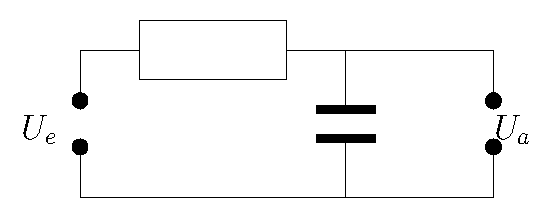
\includegraphics[width=0.2\textwidth]{bilder/schalt_tiefpass}}
      \subfigure[\label{abb_schalt_hochpass}Schaltung
      Hochpass]{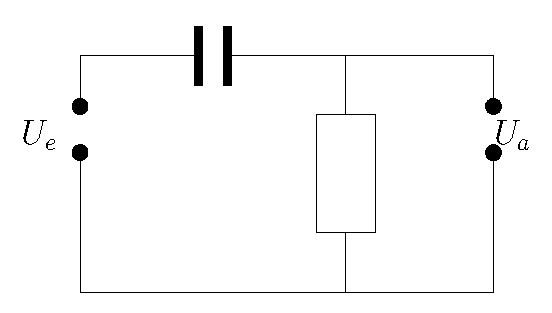
\includegraphics[width=0.2\textwidth]{bilder/schalt_hochpass}}
\subfigure[Ve\label{abb_hochtiefpass}rh"altnis $|U_a / U_e|$ bez"uglich Frequenz
$\omega$]{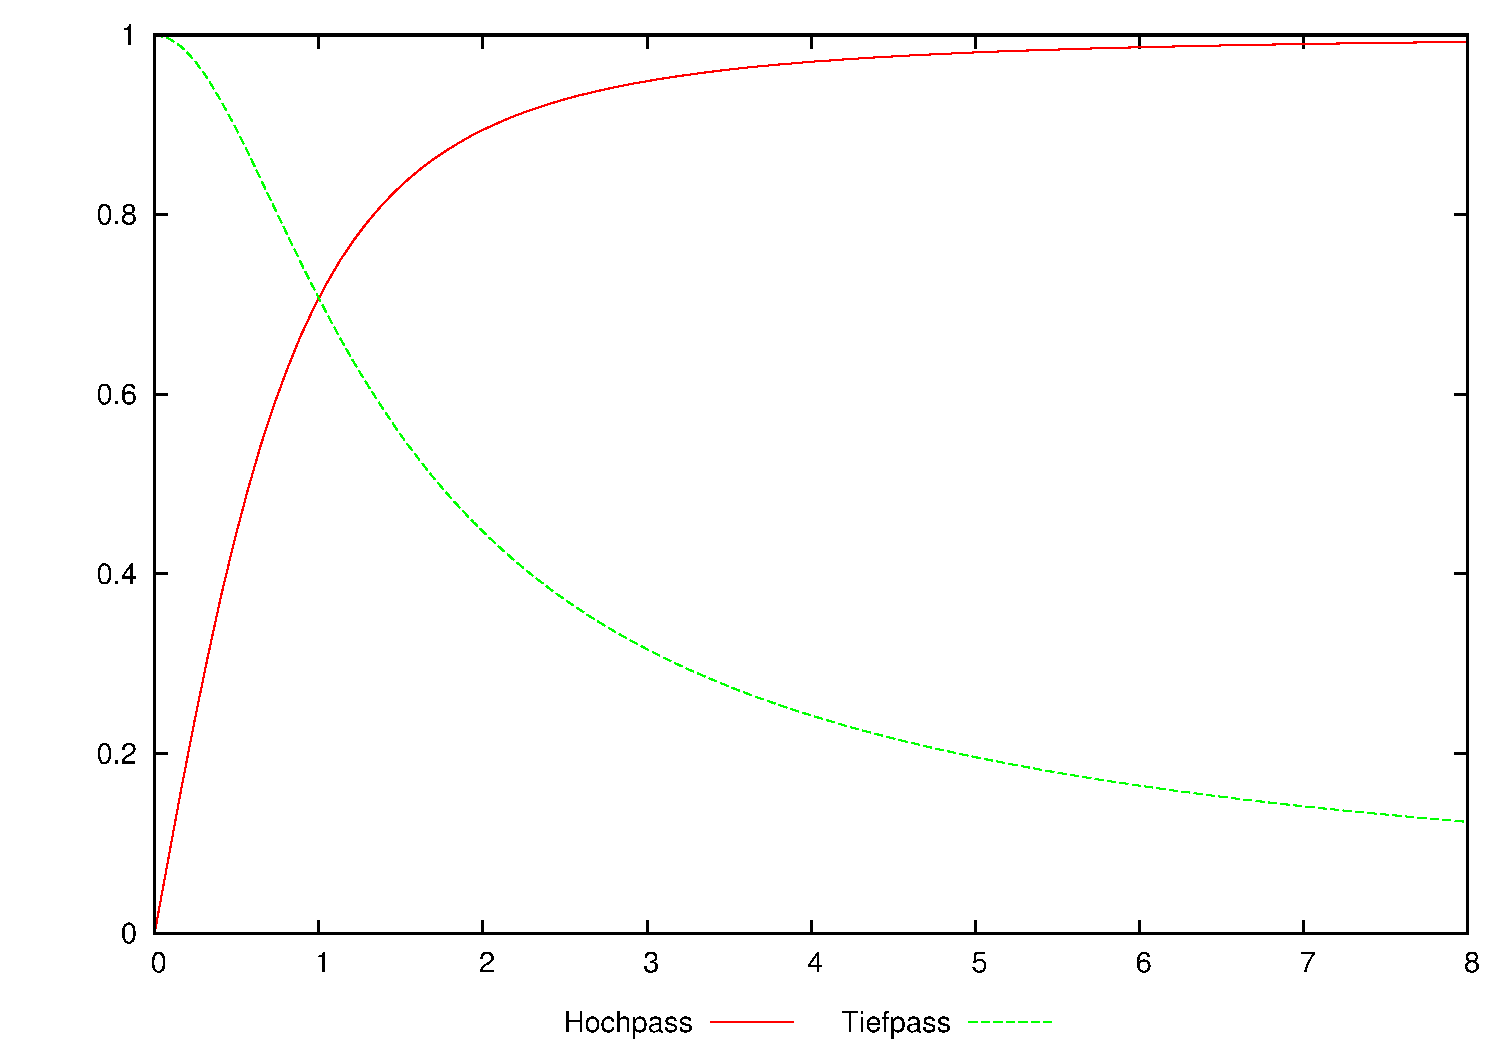
\includegraphics[width=0.5\textwidth]{bilder/hochtiefpass2}}
      \caption{Hoch- und Tiefpass mit Kondensator}
      \label{abb_hoch-tiefpass_kond}
   \end{figure}
\end{Beispiel}






\subsection{Transformator}
\label{kap_transformator}

An einem \index{Eisenjoch}Eisenjoch\footnote{viereckiger
  Donought} sind an zwei Seiten zwei Spulen mit verschiedenen
Windungszahlen $N_i$ angebracht. Legt man an eine eine Wechselspannung
$U_1$ an, so erh"alt man an der anderen ebenfalls eine Spannung $U_2$:
Die erste Spule erzeugt ein sich "anderndes B-Feld, welches in der
zweiten Spule $U_2$ induziert.

F"ur die erste Spule gilt mit Maschenregel:
\begin{equation}
   \label{eq:360}
   U_1 + U_{i,1} = 0
\end{equation}
und f"ur die Induktionsspannungen gilt:
\begin{equation}
   \label{eq:365}
   U_{i,1} = -N_1 \cdot \dot \Phi_B \text{ und } U_{i,2} = -N_2 \cdot
   \dot \Phi_B
\end{equation}
Und weil an der Zweiten Spule nur die Induktionsspannung abf"allt:
\begin{equation*}
   \label{eq:366}
   U_2 = U_{i,2} = -N_2 \cdot \dot \Phi_B = -N_2 \cdot
   \frac{U_{i,1}}{-N_1} = - \frac{N_2}{N_1} U_1
\end{equation*}
Und damit der allgemeine Zusammenhang
\begin{equation*}
   \label{eq:367}
   {\frac{U_2}{U_1} = - \frac{N_2}{N_1}}
\end{equation*}
D.h. zwischen den beiden Spannungen liegt eine Phase von $\varphi =
\pi$, also $180^\circ$.\footnote{Diese Phasenbeziehung gilt, weil $U_2
= - \frac{N_2}{N_2}U_1$ ist; das entscheidende ist das \emph{negative}
vorzeichen. Aus $\cos\theta$ wird so $-\cos\theta$, welches einen
Phasenunterschied von $\pi$ bedeutet.}

Hat die Sekund"arspule einen angeschlossenen Stromkreis mit Widerstand
$R$, so gilt wegen der Energieerhaltung
\begin{equation*}
   U_1 I_1 = U_2 I_2
\end{equation*}
und damit
\begin{equation}
   \label{eq:368}
   \boxed{ \frac{I_1}{I_2} = \frac{U_2}{U_1} = - \frac{N_2}{N_1}}
\end{equation}




\begin{Beispiel}
   Leistungsverlust minimieren durch Hochspannungsleitungen:

   Eine Leitung hat Widerstand $R$, dann f"allt die Leistung $P = UI =
   RI^2$ ab; der relative Leistungsverlust ist (die Stromst"arke $I$
   bleibt konstant, weil ja keine Ladungen aus der Leitung entfernt werden):
\begin{equation*}
   \frac{\Delta P}{P} = \frac{\Delta UI}{UI} = \frac{\Delta U}{U}
\end{equation*}

Bei der "Ubertragung von $20\operatorname{kW}$ mit einem Leiter mit
Widerstand $R = 2.125\Omega$ ergibt sich
\begin{description}[\setlabelstyle{\bfseries\slshape}]
\item[Bei 230V] $I =\frac{P}{V}= 87\operatorname{A}$ und $\Delta U = RI =
   185\operatorname{V}$, also $\frac{\Delta U}{U} = 0.80$
\item[Bei 20 kV] $I = 1\operatorname{A}$ und $\Delta U = 2,125
   \operatorname{V}$, also $\frac{\Delta U}{U} = 1.1 \cdot 10^{-4}$.
\end{description}
Der relative Leistungsverlust ist also weit geringer bei hohen Spannungen.
\end{Beispiel}







\subsection{Der Elektrische Schwingkreis}
\label{kap_elektrische-schwingkreis}

In einem Stromkreis liegen Spule $L$, Kondensator $C$ und Widerstand
$R$ vor, au"serdem ein Schalter $S$. Der Kondensator wird geladen und
der schalter bei $t =0$ geschlossen.

Der gemessene Strom schwingt: $C$ entl"adt sich --  wegen $U_i$ der
Spule nur langsam. Ist $C$ entladen, sollte der Strom abbrechen, wird
aber von $U_i$ aufrecht erhalten, wodurch $C$ wieder entgegengesetzt
geladen wird usw.

\begin{Wichtig}
   Es wird st"andig Elektrische Energie ($W = \frac{1}{2}CU^2$) in
   Magnetische ($W = \frac{1}{2}LI^2$) umgewandelt.
\end{Wichtig}

Diesen Aufbau haben wir in
Kap. \ref{kap_schaltungen-mit-komplexen-widerstanden} behandelt. In
Gl. \eqref{eq:356} k"onnen wir deshalb einfach $U = 0$ setzen:
\begin{equation}
   \label{eq:369}
   \frac{1}{C}I + R \dot I + L\ddot I = 0
\end{equation}
Der Ansatz ist nun
\begin{equation*}
   I(t) = A \E^{\lambda t} \text{ und so } \dot I = \lambda I \text{
     und } \ddot I = \lambda^2 I
\end{equation*}
Durch Einsetzen folgt das \index{charakteristisches
  Polynom}charakteristische Polynom
\begin{equation}
   \label{eq:370}
     \frac{1}{C} + R \lambda + L \lambda^2 = 0
\end{equation}
mit den L"osungen
\begin{equation}
   \label{eq:371}
   \lambda_{1,2} = -\frac{R}{2L} \pm \frac{1}{2L}\sqrt{R^2 -
     4\frac{L}{C}}
=
-\underbrace{\frac{R}{2L}}_\alpha \pm \underbrace{\sqrt{\frac{R^2}{4L^2} -
     \frac{1}{CL}}}_\beta
\end{equation}
Und damit ist die L"osung der eine Linearkombination der bisher
gefundenen L"osungen:
\begin{equation}
   \label{eq:372}
   I(t) = A_1 \E^{-(\alpha + \beta)t} + A_2 \E^{-(\alpha - \beta)t}
\end{equation}
Wir unterscheiden die folgenden F"alle:
\begin{description}[\setlabelstyle{\bfseries\slshape}]
\item[\index{Kriechfall}Kriechfall] $\frac{R^2}{4L^2} > \frac{1}{LC}$ bzw. $R^2 > 4{\frac{L}{C}}$: $\beta \in
   \mathbb R$ und damit $\lambda \in \mathbb R$. $I$ f"allt einfach
   exponentiell ab.
\item[\index{Aperiodischer Grenzfall}Aperiodischer Grenzfall]  $R^2 = 4\frac{L}{C}$ und
   damit $\beta = 0$. Die L"osung ist
   \begin{equation}
\label{eq:374}
      I(t) = \E^{-\alpha t} \left (A_1 + A_2 \cdot t \right )
   \end{equation}
\item[\index{Ged"ampfte Schwingung}Ged"ampfte Schwingung] $R^2 < 4\frac{L}{C}$: $\beta \in \mathbb
   C\backslash \mathbb R$ und damit $\lambda \in \mathbb C\backslash
   \mathbb R$. $\beta \equiv \I \omega$ und
   \begin{equation*}
      I (t) = \E^{-\alpha t} \left ( A_1 \E^{\I \omega t} + A_2 \E^{-\I
         \omega t} \right ) \text{ mit } \bar A_1 = A_2
   \end{equation*}
   (Die zeite Bedingung machen wir, damit wir eine reelle L"osung
   bekommen.) Damit kann man dies umformen zu
  \begin{equation}
     \label{eq:373}
     I(t) = \E^{-\alpha t} |A| \cos (\omega t + \varphi)
  \end{equation}
D.h. eine abklingende, harmonische Schwingung mit der Frequenz
\begin{equation}
   \label{eq:375}
   \omega = \sqrt{- \frac{R^2}{4L^2} +
     \frac{1}{CL}} \text{ und der Eigenfrequenz } \omega_0 = \sqrt{\frac{1}{CL}}
\end{equation}
\end{description}
%
Legt man eine "au"sere Spannung $U$ an, so hat man eine
\textbf{erzwungene Schwingung} mit Gl. \eqref{eq:356}. Aus
Kap. \ref{kap_schaltungen-mit-komplexen-widerstanden} wissen wir
(Gl. \eqref{eq:362}), den Gesamtwiderstand $Z$ und die Phase $\varphi$
des Systems. Untersuchen wir dies auf die Abh"angigkeit der Frequenz
$\omega$, so ergibt sich dass $|Z|$ minimal wird, wenn $\omega \to
\omega_0$; dann verschwindet der Imagin"arteil von $Z$. Der Realteil ,
$R$, wird von der Frequenz nicht ver"andert! F"ur $\omega \to \omega_0$
verschwindet auch die Phase.

Man kann eine \textbf{\index{gekoppelte Schwingung}gekoppelte
  Schwingung} erzeugen, indem man die Spulen zweier Schwingkreise
nebeneinander h"alt, damit diese ineinander Spannungen induzieren, oder
indem sich die Schwingkreise einen Kondensator teilen.


\abs
All diese Rechnungen verlaufen analog zu denen aus
Kap. \ref{kap_schwingungen-und-wellen}.









\section{Materie im B-Feld}
\label{kap_materie-im-b-feld}

Wird eine Luftspule von Strom durchflossen, etabliert sich
gem. Gl. \eqref{eqn_B-spule} das B-Feld
\begin{equation*}
   B_0 = \mu_0 I \frac{N}{L}
\end{equation*}
F"uhrt man nun Materie ein, so steigt $B$
an.\footnote{\emph{Eigentlich} bemerkt man nur, dass sich $\Phi_B =
  \int_A \vec B \diff \vec A$ "andert, aber da $A$ bei dem Versuch
  konstant bleibt, muss sich $B$ "andern.} Analog zu $\varepsilon_r$
(vgl Kap. \ref{kap_isolatoren-im-e-feld}) definiert man:
\begin{Def}
   [\index{relative Permeabilit"at}relative Permeabilit"at $\mu_r$] Ist
   der Quotient der B-Feldst"arke mit ($B$) und ohne ($B_o$) Materie:
   \begin{equation}
      \label{eqn_def_mu_r}
      \mu_r = \frac{B}{B_0} \text{ oder } B_\text{Materie} = \mu_r
      \cdot B_\text{Vakuum}
   \end{equation}
\end{Def}
$\mu_r$ ist eine \emph{dimensionslose} Materialkonstante: $[\mu_r] =
1$.

Wie im E-Feld, wo Dipole des Dielektrikums ausgerichtet wurden, werden
vom angelegten B-Feld magnetische Pole mit den Momenten $\vec \mdm$
ausgerichtet; diese sorgen nun selbst f"ur eine magnetische
Eigenschaft, die man als \textbf{\index{Magnetisierung}Magnetisierung}
$\vec M$ bezeichnet (analog zur
\emph{\index{Polarisierung}Polarisierung} $\vec
P$):\footnote{Verwendet man die Schreibweise $\vec m = \vec \mdm$ so
  f"uhrt dies zu der etwas verwirrenden Schreibweise $\vec M = n \vec m$.}
\begin{equation}
   \label{eqn_def_magnetisierung}
   \vec M = \frac{1}{V} \sum_V \vec \mdm ~ ~ \text{ wenn alle $\vec \mdm$
     parallel: } \boxed{\vec M = n \cdot \vec \mdm}
\end{equation}
Mit der Einheit $[M] = \frac{\operatorname{A}}{\operatorname{m}}$.

Das B-Feld in der Materie ist nun\footnote{Vergleiche $E_D = E_0 - \frac{P}{\varepsilon_0}$}
\begin{equation}
   \label{eq:378}
   \vec B = \vec B_0 + \mu_0 \cdot \vec M = \mu_0 \left (\vec H + \vec
      M \right )
\end{equation}
Wobei $\vec H = \frac{1}{\mu_0} \vec B_0$ (bzw in Materie: $\vec H =
\frac{1}{\mu_0 \mu_r}\vec B$) die \textbf{magnetische Erregung} ist,
die wir bereits aus Kap. \ref{kap_magnetische-feld} kennen.

Experimentell ergibt sich, dass bei nicht zu gro"sen Feldst"arken
\begin{equation}
   \label{eq:379}
   \vec M = \chi \cdot \vec H_0
\end{equation}
ist mit:
\begin{Def}
   [\index{Magnetische Suszeptibilit"at}Magnetische Suszeptibilit"at
   $\chi$] Ist eine Materialkonstante, welche angibt, wie gut ein
   Stoff durch ein externes B-Feld zu magnetisieren ist.
\end{Def}
$\chi$ hat keine Einheit: $[\chi] = 1$.

Dabei wissen wir bereits, dass $B_0 = \mu_0 H_0$ und damit
\begin{equation}
   \label{eq:380}
   \vec B = \mu_r \vec B_0 = \mu_0 \mu_r \cdot \vec H_0
\end{equation}
Setzt man \eqref{eq:379} in \eqref{eq:378} ein, liefert ein
Koeffizientenvergleich mit \eqref{eq:380} den Zuammenhang
\begin{equation}
   \label{eq:381}
   \mu_r = 1 + \chi
\end{equation}



\subsection{Arten der Magnetisierung}
\label{kap_arten-magnetisierung}

Nach der Gr"o"se von $\chi$ (also ihrer Magnetisierbarkeit) ordnet man
verschiedene Stoffe ein in die Kategorien:
\begin{description}[\setlabelstyle{\bfseries\slshape}]
\item[Diamagnetische Stoffe] $|\chi| \ll 1$, $\chi < 0$

Schw"achen ext. B-Feld ab: Aus $\chi < 0$ folgt $\mu_r < 1$ und $B < B_0$.

Bsp.: Helium, Neon, argon, Xenon, Wasserstoff, Stickstoff, Bismut.

\bigskip

Dieser Effekt trifft eigentlich \emph{immer}, also in allem
Materialien auf und ist bei Stoffen ohne permamentes magnetisches
Dipolmoment wichtig.

Wird das Meterial ins B-Feld gebracht, werden darin Kreisstr"ome
induziert, die (nach \textsc{Lenz}'scher Regel) dem externen B-Feld
entgegenwirken.

Ein St"abchen Diamagnet w"urde im B-Feld rotieren, bis es senkrecht zum
B-Feld steht. Gase werden aus dem B-Feld gedr"angt.
\item[Paramagnetische Stoffe]  $|\chi| \ll 1$, $\chi > 0$

Verst"arken B-Feld: Aus $\chi > 0$ folgt $\mu_r > 1$ und $B > B_0$.

Bsp.: Aluminium, Natrium, Mangan, Sauerstoff, Wolfram.


\bigskip

Im Material liegen permanente Dipole vor, die aber ungeordnet sind.;
wegen thermischer Bewegung der Teilchen sind die Dipole zuf"allig
orientiert und heben einander auf: $\frac{1}{V}\sum_V \vec \mdm = \vec
0 = \vec M$.

Durch ein Externes B-Feld werden die DIpole teilweise in Richtung von
$\vec B$ orientiert, damit $\vec M \| \vec B$. Der Grad der
Ausrichtung (also $\|\vec M\|$) ist \emph{temperaturabh"angig}. Die
Parallel und antiparallel ausgerichteten Teilchen bilden eine
\textsc{Boltzmann}-Verteilung
\begin{equation}
   \label{eq:382}
   \frac{n_\text{antipar}}{n_\text{parallel}} = \exp \left ( -
      \frac{E_\text{antipar} - E_\text{parallel}}{K_B \cdot T} \right
   ) \text{ mit } E = \vec \mdm \cdot \vec B
\end{equation}

und es gilt f"ur kleine Energiedifferenzen ($\Delta E \ll K_B \cdot T$)
\begin{Wichtig}
   \textbf{\textsc{Curie}-Gesetz}:
   \begin{equation}
      \label{eq:383}
      \chi \sim \frac{1}{T}
   \end{equation}
\end{Wichtig}

Ein St"abchen Paramagnet rotiert, bis es parallel zum B-Feld steht.

\item[Ferromagnete]  $|\chi| \gg 1$, $\chi > 0$

Verst"arken B-Feld \emph{deutlich}.

Bsp.: Eisen, Nickel.

\bigskip

Wie beim Permamagnetismus liegen hier permanente Dipole
vor. \emph{Aber:} Zus"atzlich zur Ausrichtung von Au"sen beeinflussen
sich die einzlenen Elemtarmagnete: Zwischen ihnen wirkt eine
Austauschwechselwirkung.

Die einzelnen Dipole bilden \textsc{\index{Wei"ssche Bezirke}Wei"s}'sche
Bezirke; also Bereiche, in denen alle $\vec \mdm$ parallel ausgerichtet
sind.

Die Magnetisierung ist wieder stark von der Temperatur abh"angig. Bei
hohen Temperaturen verh"alt sich ein Ferromagnet wie ein
Permanentmagnet. Die Austauschwechselwirkungsenergie $E_A$, die f"ur
Ordnung sorgt, wirkt gegen
die Thermische Energie $K_B T$ an, die f"ur Unordnung sorgt. "Uberhalb
der \textbf{\textsc{\index{Curietemperatur}Curie}-Temperatur} $T_C$
ist $E_A < K_BT$. Hier kann $\chi(T)$ n"ahrungsweise beschrieben werden
durch:
\begin{Wichtig}
   [\textsc{Curie-Wei"s}'sches Gesetz] F"ur $T > T_C$ gilt:
   \begin{equation}
      \label{eq:384}
      \chi = \frac{C}{T - T_C}
   \end{equation}
mit der materialabh"angigen \textbf{\textsc{Curie}temperatur} $T_C$ und
der materialabh"angigen \textbf{\textsc{Curie}konstanten} $C$.
\end{Wichtig}


\begin{figure}[h]
   \centering
   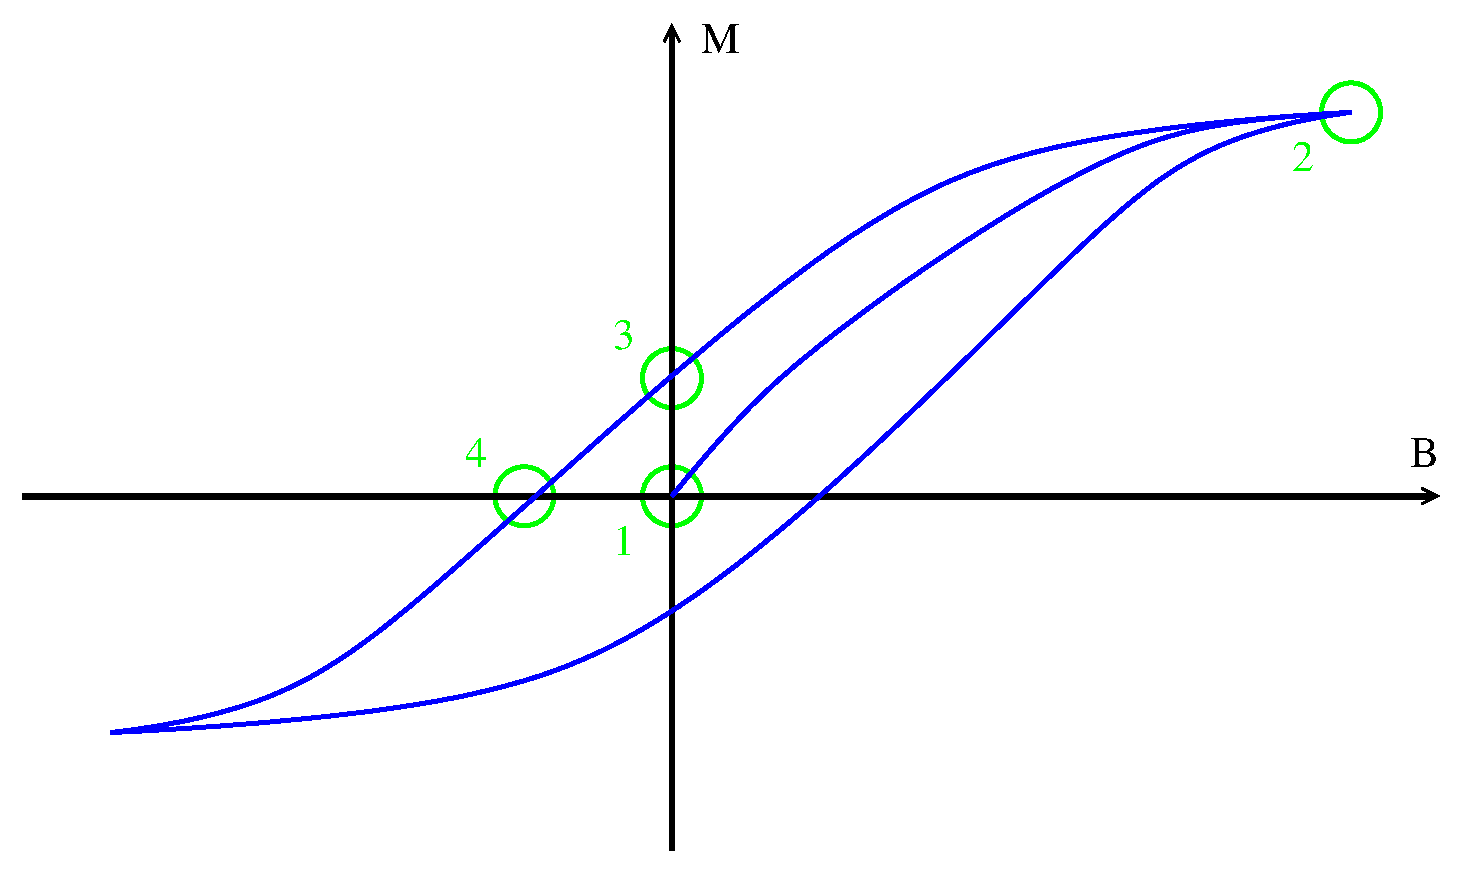
\includegraphics[width=0.7\textwidth]{bilder/hysterese_ferro}
   \caption{Hysteresekurve der Magnetisierung eines Ferromagneten}
\label{abb_hysterese_ferro}
\end{figure}

Magnetisiert man einen Ferromagneten mit einem "au"seren B-Feld, so
bleibt danach eine restmagnetisierung "ubrig: Man hat einen Magneten
"`erschaffen"'. Dies bezeichnet man als
"`\index{Hysterese"'}Hysterese"': Die Ausgangsgrr"o"se ($M$) h"angt nicht
nur von der Eingangsgr"o"se ($B$) ab, sondern auch von der
\emph{Geschichte}, welche die Eingangsgr"o"se hatte. Man unterscheidet
vier verschiedene Zust"ande:
\begin{enumerate}
\item $\vec M = \vec 0$ wird dadurch erreicht, dass die Probe
   aufgeheizt wird und "uberhalb von $T_C$ ihre magnetischen
   Eigenschaften verliert. K"uhlt man schnell genug ab, so bleibt die
   Unordnung und damit $\vec M = \vec 0$ erhalten.
\item $\vec B$ wird erh"oht: Die Dipole richen sich parallel zu $\vec
   B$ aus, bis die \textbf{\index{S"attigung}S"attigung} erreicht ist:
   Dann sind alle Dipole ausgerichtet.
\item Wegen den Austauschwechselwirkungen bleiben die Dipole teilweise
   ausgerichtet. Bei $\vec B = \vec 0$ hat man noch eine endliche
   Magnetisierung $\vec M$. diese hei"st \textbf{\index{Rimanenz}Rimanenz}.
\item Um die Magnetisierung auszul"oschen ist sogar ein Gegenfeld $\vec
   B'$ n"otig; Hier ist $\vec M (\vec B') = \vec 0$. $\vec B'$ nennt
   man \textbf{\index{Koerzitivfeldst"arke}Koerzitivfeldst"arke}.
\end{enumerate}
Um die Hysteresekurve zu messen baut man das Joch eines Transformators
aus dem entsprechenden Material und legt das B-Feld an: $U \sim -N
\dot \Phi_B \sim \dot B_\text{Spule} \sim \dot M$, au"serdem $U \sim I$ in der
Spule. Damit ist $I \sim M$.

\item[Antiferromagnete]  $|\chi| \ll 1$, $\chi > 0$

Schw"achen B-Feld \emph{deutlich} ab.

\bigskip

Im Stoff liegen permanent magnetische Dipole $\vec \mdm$ vor. Ist kein
"au"seres Feld angelegt, gleichen sie sich aus: Did Dipole sind
paarweise antiparallel ausgerichtet, damit ist $\vec M = \vec 0$.
\end{description}











\section{Die \textsc{Maxwell}'schen Gleichungen}
\label{kap_maxwellschen-gleichungen}

Das \textsc{Amp\`ere}'sche Gesetz ($ \oint_\gamma \vec B \diff \vec s
= \mu_0 I$; vgl. \eqref{eqn_gesetz_ampere}) f"uhrt bei
Wechselstromkreisen zu Widerspr"uchen: Betrachtet man einen
Kondensator und integriert einmal um den Leiter ($\gamma_1$) und
einmal einen Kreis zwischen den Platten ($\gamma_2$), so m"usste
zwischen den Platten das B-Feld verschwinden ($B(\gamma_2) = 0$), weil
$I(\gamma_2) = 0$; trotzdem ist aber $B(\gamma_1) \neq 0$. F"ur
Wechselstrom muss demnach eingef"uhrt werden:
\begin{Def}
   [\index{Verschiebungsstrom}\index{Verschiebungsstromdichte}Verschiebungsstrom(dichte)
   $I_v$ ($\vec j_v$)] Flie"st der Strom $I$ durch einen Kondensator, so werden
   Ladungen $q$ von den und auf die Platten bewegt. Es etabliert sich
   ein E-Feld $E = \frac{\sigma}{\varepsilon_0} = \frac{q}{A\cdot
     \varepsilon_0}$ bzw. $q = A \cdot \varepsilon_0 \cdot E$, welches
   den Verschiebungsstrom hervorruft:
   \begin{equation}
      \label{eqn_def_verschiebungsstrom}
      I_v = \frac{\partial q}{\partial t } = A \cdot \varepsilon_0
      \cdot \frac{\partial E}{\partial t} = \varepsilon_0
      \frac{\partial }{\partial t} \int_A \vec E \diff \vec A ~ ~ \text{ und } ~ ~ \vec
      j_v = \varepsilon_0 \cdot \frac{\partial \vec E}{\partial t}
   \end{equation}
\end{Def}
Weniger anschlaulich, daf"ur korrekter ist die Definition
  \begin{equation*}
     I_v = \varepsilon_0 \varepsilon_r \, \frac{\diff
       \Phi_E}{\diff t}
     =
     \varepsilon_0 \varepsilon_r \, \frac{\diff
     }{\diff t} \int_A \vec E \diff \vec A 
     =
     \varepsilon_0 \varepsilon_r \, \int_A \frac{\partial }{\partial t}\vec E \diff \vec A 
  \end{equation*}
Ein Koeffizientenvergleich mit $I = \int_A \vec j \diff \vec A$ aus
\eqref{eq:300} liefert nun \eqref{eqn_def_verschiebungsstrom} (wobei
wir hier noch ein $\varepsilon_r$ eingef"uhrt haben -- in
\eqref{eqn_def_verschiebungsstrom} befinden wir uns im Vakuum mit
$\varepsilon_r = 1$. Hier
sieht man, dass  der Verschiebunsstrom ein Analogon zur
Induktionsspannung beim B-Feld ist; vgl \eqref{eq:329}.

Addiert man diese Gr"o"se beim \textsc{Amp\`ere}'schen Gesetz, so gilt
dieses auch f"ur Wechselstrom:\footnote{Wenn $E$ gen"ugend stetig ist,
  dass man ableitung und Integral vertauschen darf.}
\begin{equation}
   \label{eqn_gesetz_ampere_allg}
   \oint_\gamma \vec B \diff \vec s = \mu_0 (I + I_v) = \mu_0 \int_A
   (\vec j + \vec j_v) \diff \vec A = \mu_0I + \mu_0 \varepsilon_0
   \frac{\partial }{\partial t} \int_A \vec E \diff \vec A
\end{equation}
Dabei hei"st $I$ \emph{\index{Leitungsstrom}Leitungsstrom}. Der letzte
Ausdruck f"ur den Verschiebungsstrom gilt f"ur beliebige Kondensatoren.

Damit k"onnen wir die \textsc{Maxwell}-Gleichungen formulieren:


\clearpage

\begin{Wichtig}[\textsc{\index{Maxwell-Gleichungen!Integralform}Maxwell}-Gleichungen in Integralform]~\\
   \begin{enumerate}[(I)]
   \item Satz von \textsc{Gauss}: Ladungen sind Quellen des E-Felds:
\begin{equation}
   \label{eqn_max1_int}
   \oint_A \vec E \diff \vec A = \frac{1}{\varepsilon_0} \int_V
   \varrho_q \diff V
\end{equation}
\item B-Felder sind quellenfrei, Feldlinien sind in sich geschlossen:
   \begin{equation}
      \label{eqn_max2_int}
      \oint_A \vec B \diff \vec A = 0
   \end{equation}
\item Induktionsgesetz ($U_i = -\frac{\partial }{\partial
     t}\Phi_B$ umgeschrieben): Zeitlich ver"anderliches B-Feld induziert E-Feld
   (bzw. Spannung):
   \begin{equation}
      \label{eqn_max3-int}
      \oint_\gamma \vec E \diff \vec s = -\frac{\partial }{\partial t}
      \int_A \vec B \diff \vec A
   \end{equation}

\item \textsc{Amp\`ere}'sches Gesetz: Zeitlich ver"anderliche E-Felder
   erzeugen B-Felder:
   \begin{equation}
      \label{eqn_max4-int}
      \oint_\gamma \vec B \diff \vec s = \mu_0 \int_A \left(\vec j +
      \varepsilon_0\frac{\partial }{\partial t}\vec E\right) \diff \vec A
   \end{equation}
   \end{enumerate}
\end{Wichtig}

Wendet man die S"atze von \textsc{Gauss}
(Kap. \ref{kap_satz-von-gauss}) [f"ur die ersten beiden Gl.] und \textsc{Stokes}
(Kap. \ref{kap_satz-von-stokes})  [f"ur die beiden letzten Gl.] auf die Integrale an, erh"alt man die
differenzielle Form:

\begin{Wichtig}
   [\textsc{\index{Maxwell-Gleichungen!Differenzialform}Maxwell}-Gleichungen
   in Differenzial-Form]~\\
   \begin{enumerate}[(i)]
   \item Ladungen sind Quellen des E-Felds
      \begin{equation}
         \label{eqn_max1-diff}
         \vec \nabla \, \vec E = \frac{1}{\varepsilon_0} \varrho_q
      \end{equation}

   \item B-Feld hat keine Quellen
      \begin{equation}
         \label{eqn_max2-diff}
         \vec \nabla \, \vec B = 0
      \end{equation}


   \item "Anderung des B-Felds induziert "anderung des E-Felds
      \begin{equation}
         \label{eqn_max3-diff}
         \vec \nabla \times \vec E = - \frac{\partial }{\partial t}
         \vec B
      \end{equation}

   \item Bewegte Ladungen und zeitlich "andernde E-Felder erzeugen
      B-Feld; B-Feld ist Wirbelfeld.
      \begin{equation}
         \label{eqn_max4-diff}
         \vec \nabla \times \vec B = \mu_0 \left ( \vec j +
            \varepsilon_0 \frac{\partial }{\partial t} \vec E \right)
      \end{equation}

   \end{enumerate}
\end{Wichtig}


\begin{Wichtig}
Zusammen mit der \textsc{Lorentz}kraft
\begin{equation*}
   F = q (\vec E + \vec v \times \vec B)
\end{equation*}
und $\vec F = m\vec a$ kann man damit alle elektromagnetischen
Ph"anomene beschreiben.
\end{Wichtig}




\subsection{Neues Potential, DGLs entkoppeln ($\bigstar$)}
\label{kap_neues-potential}


Liegt ein zeitlich ver"anderliches B-Feld vor, so bildet das E-Feld ein
Wirbelfeld (\eqref{eqn_max3-diff}) bzw. die Rotation verschwindet
nicht mehr und somit kann man kein (elektrisches) Potential
$\varphi$ mehr finden sodass
\begin{equation*}
   \vec E = - \vec \nabla \, \varphi
\end{equation*}
Stattdessen hat man in Gl. \eqref{eqn_max3-diff}
\begin{equation*}
   \label{eq:385}
   \vec\nabla \times \vec E + \frac{\partial }{\partial t}\vec B = 0
\end{equation*}
Da wir das Vektorpotential $\vec \Apot$ definiert haben
\eqref{eq:303}, k"onnen wir $\vec B = \vec\nabla\times \Apot$
verwenden, indem wir $\vec\nabla\times \cdot$ mit $\frac{\partial
}{\partial t}$ vertauschen (wir setzen wieder eine ausreichende
Glattheit voraus):
\begin{equation}
   \label{eq:386}
   \frac{\partial }{\partial t}\vec B = \frac{\partial }{\partial t}
   \vec\nabla\times\vec\Apot = \vec\nabla\times \frac{\partial
   }{\partial t} \vec\Apot
\end{equation}
Und dies in \eqref{eqn_max3-diff} eingesetzt, liefert
\begin{equation}
   \label{eq:387}
   \vec\nabla\times \vec E + \vec \nabla \times \frac{\partial }{\partial t}{\vec \Apot} =
   \vec\nabla\times \left (\vec E + \frac{\partial }{\partial t }{\vec \Apot} \right)= 0
\end{equation}
Es verschwindet also die Rotation von $(\vec E + \frac{\partial
}{\partial t }{\vec \Apot})$
und damit k"onnen wir dies mithilfe eines Skalaren Potentials
$\phi_{el}$ schreiben:
\begin{equation}
   \label{eq:388}
    \left (\vec E + \frac{\partial }{\partial t}{\vec \Apot} \right)
    =: - \vec \nabla\, \phi_{el}
\end{equation}
und damit
\begin{equation}
   \label{eq:389}
   \boxed{\vec E = - \vec\nabla \phi_{el} - \frac{\partial }{\partial t}\vec\Apot}
\end{equation}
Wenn kein B-Feld vorliegt oder es zeitlich konstant ist, dann stimmt
$\phi_{el}$ mit $\varphi$ "uberein -- dies ist also ein allgemeinerer
Fall.\footnote{Wendet man die Rotation auf Gl. \eqref{eq:389} an, so
  erh"alt man daraus die Maxwell-Gleichung \eqref{eqn_max3-diff}, wenn
  man beachtet dass $\nabla \times (\nabla\, \phi_{el}) = 0$ ist.}

Wie wir in Kap. \ref{kap_vektorpotential} gesehen hatten, ist $\vec
\Apot$ durch $\vec\nabla \times \vec \Apot = \vec B$ nicht voll
definiert. Man f"uhrt deshalb die \textbf{\textsc{\index{Lorentz'sche
      Eichbedingung}Lorentz}'sche Eichbedingung} ein:
\begin{equation}
   \label{eq:390}
   \boxed{ \vec\nabla\, \vec \Apot = - \frac{1}{c_0^2}
     \frac{\partial }{\partial t} \phi_{el} } = -\varepsilon_0\mu_0    \frac{\partial }{\partial t} \phi_{el}
\end{equation}
Wendet man auf Gl. \eqref{eq:389} die Divergenz an, so folgt mit
dieser Eichbedingung und \eqref{eqn_max1-diff}:
\begin{equation}
   \label{eq:391}
   \vec\nabla \vec E
=
 \vec\nabla\left( - \vec\nabla \phi_{el} - \frac{\partial }{\partial
      t}\vec\Apot\right)
=
-\vec\nabla^2\phi_{el} - \frac{\partial }{\partial
  t}\vec\nabla\vec\Apot
=
\boxed{
-\Laplace{\phi_{el}}+\frac{1}{c_0^2}
     \frac{\partial^2 }{\partial t^2} \phi_{el}  =
   \frac{\varrho}{\varepsilon_0}
}
\end{equation}

Au"serdem folgt aus \eqref{eqn_max4-diff} mit \eqref{eq:390}:
\begin{equation*}
   \label{eq:392}
\vec\nabla\times(\vec\nabla\times\vec\Apot)
=
 \vec\nabla(\vec\nabla\,
\vec\Apot) - \Laplace{\vec\Apot}
=
- \vec\nabla\,   \frac{1}{c_0^2}
     \frac{\partial }{\partial t} \phi_{el}  - \Laplace{\vec\Apot}
=
\mu_0\vec j + \frac{1}{c_0^2}\frac{\partial }{\partial t}\vec E
\end{equation*}
Vertauscht man hier $\vec\nabla$ und $\frac{\partial }{\partial t}$
kann man \eqref{eq:388} verwenden und erh"alt nach k"urzen des $E$-Terms:
\begin{equation}
   \label{eq:393}
   \boxed{ - \Laplace{\vec\Apot} + \frac{1}{c_0^2}\frac{\partial^2
     }{\partial t^2} \vec \Apot = \mu_0 \vec j}
\end{equation}

\begin{Wichtig}[\textsc{Maxwell}-Gl. entkoppelt]
   Die \textsc{Maxwell}-Gleichungen stellen gekoppelte
   Differenzialgleichungen dar. Mit \eqref{eq:391} und \eqref{eq:393}
   und den Potentialen $\vec\Apot$ und $\phi_{el}$ hat man diese
   \emph{entkoppelt} und in Differenzialgleichungen zweiter Ordnung "uberf"uhrt.
\end{Wichtig}








\section{Offerner Schwingkreis und \textsc{Hertz}'scher Dipol}
\label{kap_offerner-schwingkreis-und-hertzscher-dipol}


\begin{figure}
   \centering
   \subfigure[Schwingkreis   \label{abb_morphose_dipol1}]{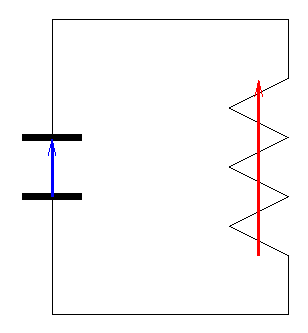
\includegraphics[height=0.15\textheight]{bilder/schwingkreis1}}
   \subfigure[Spule aufgebogen   \label{abb_morphose_dipol2}]{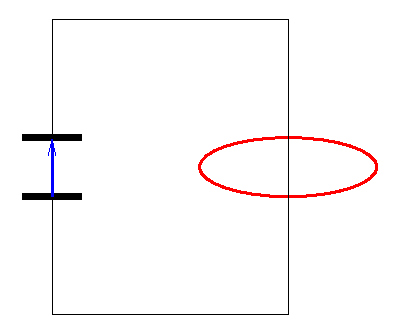
\includegraphics[height=0.15\textheight]{bilder/schwingkreis2}}
   \subfigure[Ring aufgebogen   \label{abb_morphose_dipol3}]{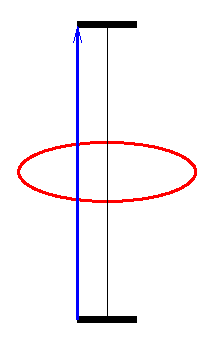
\includegraphics[height=0.15\textheight]{bilder/schwingkreis3}}
   \subfigure[Platten entfernt: \textsc{Hertz}'scher Dipol   \label{abb_morphose_dipol4}]{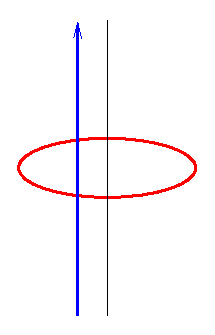
\includegraphics[height=0.15\textheight]{bilder/schwingkreis4}}
   \caption{Morphose eines Schwingkreises zu einem Hertz'schen Dipol}
   \label{abb_morphose_dipol}
\end{figure}
Wie in Abb. \ref{abb_morphose_dipol} gezeigt, handelt es sich bei
einem einfachen Draht um eine Art Schwingkreis: Die bewegten Ladungen
erzeugen Wirbel-B-Felder und an den Enden sorgen sie f"ur ein E-Feld.

Wo anfangs (\ref{abb_morphose_dipol1}) die Elektrische und
magnetische Energie noch lokal konzentriert war, breiten sich die
Felder in \ref{abb_morphose_dipol4} (mit Lichtgeschwindigkeit) im Raum
aus und damit strahlt der Dipol Energie ab.

Damit auf dem Leiter Ladungen flie"sen, muss er in der Mitte angeregt
werden (bspw kann man in die Mitte des Leiters eine kleine Spule
setzen und an diese au"sen eine Spule h"angen, die mit Wechselstrom
beschickt wird).

Weil an den Enden des Leiters der L"ange $L$, der in $z$-Richtung
ausgerichtet ist und der in der Mitte ($z = 0$) angeregt
wird, die Ladungen nicht weiter flie"sen k"onnen, gilt hier
\begin{equation*}
   I(z = \pm\frac{L}{2}) \equiv 0
\end{equation*}
und f"ur den Strom, der eine \emph{\index{Stehende Welle}Stehende
  Welle} bildet, insgesamt
\begin{equation*}
   I(z,t) = \hat I(z) \cdot \sin \omega t
\end{equation*}
Man kann die Stabenden deshalb auch als \emph{feste Enden}
bezeichnen.

Die Amplitude $\hat I (z)$ ist vom Ort auf dem Leiter abh"angig; es
gilt auch   $\hat I(z = \pm\frac{L}{2}) = 0$ wobei sich eine
Sinuswelle der Wellenl"ange
\begin{equation*}
   \lambda = \frac{2L}{n} \text{ ~ mit } n \in \mathbb N
\end{equation*}
ergibt.

In gro"ser Entfernung vom Dipol ist $\vec E$ quasi parallel zum Dipol
und $\vec B$ steht senkrecht zu $\vec E$ und liegt in einer Ebene mit
der Ausbreitungsrichtung. Wenn ein zweiter Dipol also parallel zum
ersten steht, so kann dieser als Antenne von dem E-Feld angeregt
werden. Wichtig ist dabei, dass der Dipol die Energie praktisch nur
radial abstahlt und in seine L"angsrichtung praktisch nichts.



\subsection{Abstrahlung des schwingenden Dipols}
\label{kap_abstrahlung-des-schwingenden-dipols}

Der Dipol strahlt eine \index{elektromagnetische
  Welle}elektromagnetische Welle mit der Energiedichte (auch mit $w$ bezeichnet)
\begin{equation}
   \label{eq:394}
    w_{em} = w_E + w_B= \frac{\varepsilon_0}{2}E^2 + \frac{1}{2\mu_0} B^2
\end{equation}
ab. Im Fernfeld der Welle gilt\footnote{f"allt hier vom Himmel; vgl
  dazu aber Kap. \ref{kap_magnetfeld-em-welle}!}
\begin{equation}
   \label{eq:395}
   B = \frac{1}{c_0}E
\end{equation}
und damit
\begin{equation}
   \label{eq:396}
w_{em} = \frac{1}{2} \left ( \varepsilon_0 E^2 + \frac{1}{\mu_0}
      \frac{1}{c_0^2}E^2 \right ) = \varepsilon_0 E^2
\end{equation}
\begin{Def}
   [Energiestromdichte $S$] Ist die Energie die pro Zeit durch ein
   Fl"achenelement $A$ transportiert wird:
   \begin{equation}
      \label{eq:397}
      S = \frac{W}{t \cdot A}
   \end{equation}
\end{Def}
Hier ist also
\begin{equation}
   \label{eq:398}
   S = \frac{w_{el} \cdot s}{t} = \varepsilon_0 \cdot c_0 \cdot E^2
\end{equation}
Da das Dipolmoment des Leiters wegen $I = \hat I \sin \omega t$ mit
\begin{equation*}
   \vec p(t) = \vec p_0 \cdot \sin \omega t
\end{equation*}
schwingt und die Leistung auf einer Kugeloberfl"ache mit Radius $r$
abgestrahlt wird, ergibt sich f"ur die \emph{Leistung}:\footnote{Weil
  das E-Feld sich "`nur"' mit $v = c_0$ ausbreitet, dauert es
  $\frac{r}{c_0}$, bis die "Anderung des Dipols am Punkt $r$ angekommen
  ist.}
\begin{equation}
   \label{eq:399}
   P(r) = \oint_A \vec S \diff \vec A = \frac{p_0^2 \cdot
     \omega^4}{6\pi \varepsilon_0 c_0^3} \sin^2(\omega (t -
   \frac{r}{c_0}) )
\end{equation}
Und wenn wir das zeitliche Mittel $\langle P  \rangle = \bar P$ bestimmen
wollen, verwenden wir $\langle \sin^2\theta  \rangle = \frac{1}{2}$:
\begin{equation}
   \label{eq:400}
   \bar P = \frac{p_0^2 \cdot \omega^4}{12 \pi \varepsilon_0 c_0^3} ~
   ~ \sim ~ \omega^4
\end{equation}


\begin{Beispiel}
   \begin{itemize}
   \item Ein Elektron im Atom ist praktisch ein oszillierender
      Dipol.

      Absch"atzung der Abstrahlung: Ein Lichtquant habe
      $\lambda = 500\operatorname{nm}$ und damit $W = \hbar \omega = h \nu
      = h\frac{c}{\lambda} = 4 \cdot 10^{-19}\operatorname{J}$.  Es
      ist $\bar P = \frac{W}{\tau}$ mit der Abklingzeit $\tau =
      5\cdot10^{-8}\operatorname{s}$, also $\bar P = 0.8 \cdot
      10^{-11}\operatorname{W}$.

   \item \emph{\index{R"ontgenbremsstrahlung}R"ontgenbremsstrahlung}:
      Wird ein Elektron beschleunigt, so strahlt es Energie
      "`\index{Bremsstrahlung"'}Bremsstrahlung"' ab. Werden die
      Elektronen sehr schnell auf eine Anode geschossen, so werden sie
      dort von den Elektronen des Anodenmaterials abgelenkt
      d.h. beschleunigt und strahlen Energie als R"ontgenstrahlung mit
      einem kontinuierlichen Spektrum $P(\omega)$ ab -- jenachdem, wie
      stark sie abgelenkt wurden.
   \item \emph{\index{Synchrotronstrahlung}Synchrotronstrahlung}: Ein
      Schnelles Elektron kommt in eine B-Feld und wird hier auf eine
      Kreisbahn gezwungen. Dies ist eine Beschleunigte Bewegung:
      \begin{equation*}
         evB = \frac{mv^2}{r} \text{ und so } v = \frac{e}{m} B r
      \end{equation*}
      mit $a = \frac{v^2}{r}$ folgt
      \begin{equation*}
         a = \frac{e^2}{m^2} B^2 r
      \end{equation*}
      Die abgestrahlte Leistung ist dabei proportional zu $a^2$: $P
      \sim a^2$.

      Bei kleinen Geschwindigkeiten ($v \ll c_0$) ist die
      "`Abstrahlungsverteilung"' noch "`normal"', das Elektron strahlt
      nach vorne und hinten "ahnlich viel ab. Je gr"o"ser die
      Geschwindigkeit wrid, desto st"arker werden relativistische
      Effekte, durch die die Elektronen ihre EM-Welle praktisch nur
      nach vorne mit einem sehr kleinen Raumwinkel $\Theta$ abstrahlen.


   \item \emph{Streuung einer Welle an Atomen}: Eine EM-Welle regt die
      Elektronen im Atom zum Schwingen an; es bildet sich ein Dipol:
      \begin{equation*}
         p = \alpha \cdot E = \underbrace{\alpha \cdot \hat E}_{\hat
           p} \sin \omega t = \hat p \sin \omega t
      \end{equation*}
      mit der Polarisierbarkeit $\alpha$.

      Das Dipolmoment $p$ \emph{schwingt} mit der Frequenz der
      einfallenden Welle und ist damit selbst ein Dipol, welcher eine
      EM-Welle der gleichen Frequenz abstrahlt -- aber in Alle
      Raumrichtungen senkrecht zu $\vec p$.


      Wenn der Teilchendurchmesser kleiner als die Wellenl"ange ist,
      spricht man von \emph{\textsc{Rayleight}streuung}; In
      Gl. \eqref{eq:400} kann man $p = \alpha E$ und $\omega =
      2\pi\frac{c}{\lambda}$ einsetzen und erh"alt
      \begin{equation*}
         \bar P \sim \frac{1}{\lambda^4} \text{ und } \bar P \sim E^2
      \end{equation*}
      Hier sieht man: Kurzwelliges Licht wird st"arker gebrochen weil
      $\bar P$ gr"o"ser ist! Deswegen ist der Himmel f"ur uns blau:
      Wei"ses Sonnenlicht wird "uber der Erde gebrochen und der blaue
      Anteil nach unten abgelenkt, der rote Anteil geht weiter ins Weltall.

   \end{itemize}
\end{Beispiel}







\section{EM-Welle im Vakuum}
\label{kap_em-welle-im-vakuum}

\subsection{Die Wellengleichung}
\label{kap_wellengleichung}


Im Vakuum sind keine Teilchen und damit auch keine Ladungen vorhanden:
$\varrho = 0$. Es k"onnen so auch keine Ladungen bewegt werden: $\vec j
= \vec 0$.

Wir wenden die Rotation auf die
III.\textsc{Maxwell}gl. \eqref{eqn_max3-diff} an und verwenden, dass
wegen der I. \textsc{Maxwell}gl. $\vec\nabla\, \vec E = 0$ ist, weil
ja keine Ladungen vorliegen:
\begin{equation}
   \label{eq:401}
   \vec\nabla\times (\vec\nabla\times \vec E) =
\vec\nabla(\vec\nabla\, \vec E) - \Laplace{\vec E} = -\Laplace{\vec E}
=
-\frac{\partial }{\partial t} \vec\nabla\times \vec B
\end{equation}
Setzt man nun die IV. \textsc{Maxwell}gl \eqref{eqn_max4-int} ein,
und beachtet $\vec j = \vec 0$, erh"alt man:
\begin{equation*}
   \label{eq:402}
   -\Laplace \vec E = -\frac{\partial }{\partial t} \mu_0\varepsilon_0
   \frac{\partial }{\partial t} \vec E
\end{equation*}
oder die
\begin{Wichtig}
[{\index{Wellengleichung im Vakuum}Wellengleichung im Vakuum}]
\begin{equation}
   \label{eqn_wellengleichung_vakuum}
   \boxed{ \Laplace \vec E = \mu_0\varepsilon_0 \frac{\partial^2
     }{\partial t^2} \vec E = \frac{1}{c_0^2} \frac{\partial
       ^2}{\partial t^2}\vec E}
\end{equation}
\end{Wichtig}

Beispielsweise gilt alleine f"ur $E_x$:
\begin{equation*}
   \frac{\partial^2 E_x}{\partial x^2}
+    \frac{\partial^2 E_x}{\partial y^2}
+    \frac{\partial^2 E_x}{\partial z^2}
=
\frac{1}{c_0^2} \frac{\partial ^2 E_x}{\partial t^2}
\end{equation*}
Die L"osung ist eine Welle, welche in Zeit und Raum schwingt.

Eine analoge Gleichung findet man auch f"ur das B-Feld, wenn man die
Rotation auf die IV. \textsc{Maxwell}gl. \eqref{eqn_max4-diff} anwendet.





\subsection{Ebene, periodische Welle}
\label{kap_ebene-periodische-welle}

Die Welle h"angt nur von der $z$-Koordinate und der Zeit ab:
\begin{equation}
   \label{eq:404}
   \vec E = \vec E_0 \cdot \E^{\I(kz - \omega t)}
\end{equation}
Hier bilden Real- und Imagin"arteil jeweils l"osungen der
DGL. \eqref{eqn_wellengleichung_vakuum}.

\begin{Def}
   [Wellenvektor $\vec k$] Der Wellenvektor gibt die Richtung an, in
   die sich eine Welle ausbreitet. Der Betrag ist $\|\vec k\| =
   \frac{2\pi}{\lambda}$. Man kann eine Welle folgenderma"sen
   beschreiben:
   \begin{equation}
      \label{eq:403}
      \vec E = \vec E(\vec r, t) = \vec A_0 \cdot \E^{\I (\vec k\cdot
        \vec r - \omega t)}
   \end{equation}
\end{Def}
f"ur $\vec k = (0,0,k)^T$ sind die Gl. \eqref{eq:403} und \eqref{eq:404}
identisch.

Bei der Welle handelt es sich um eine
\emph{\index{Transversalwelle}Transversalwelle} (also $\vec E \bot
\vec k$), bei der $\vec E \bot
\vec B$ ist.
\begin{Wichtig}
   Die Welle ist in Materie nicht mehr unbedingt eine Transversalwelle.
\end{Wichtig}





\subsection{Polarisation vom EM-Wellen}
\label{kap_polarisation-vom-em-wellen}

Wir betrachten eine Welle, die sich nach $z$ ausbreitet;
vlg. \eqref{eq:404}. Hier kann $\vec E_0$ irgendwo in der $xy$-Ebene
liegen. Die Orientierung von $\vec E$ ist durch \textbf{Polarisation}
der Welle bestimmt:
\begin{description}[\setlabelstyle{\bfseries\slshape}]
\item[\index{Lineare Polarisation}Lineare \index{Polarisation}Polarisation]
$\vec E_0$ zeigt immer in die selbe Richtung:
\begin{equation}
\label{eq:405}
   \vec E_0 = (E_0^{(x)}, E_0^{(y)}, 0)^T
\end{equation}
Dann ist
\begin{equation*}
   \vec E = \vec E(\vec r,t) =
   \begin{pmatrix}
      E_x\\E_y\\E_z
   \end{pmatrix}
=
\begin{pmatrix}
   E_0^{(x)} \cdot \E^{\I (k z - \omega t)}\\
   E_0^{(y)} \cdot \E^{\I (k z - \omega t)}\\
0
\end{pmatrix}
\end{equation*}
D.h die $x$ und die $y$-Komponenten schwingen in Phase.
\item[\index{Zirkulare Polarisation}Zirkulare Polarisation]
Die Betr"age von $E_0^{(x)}$ und $E_0^{(y)}$ sind gleich, die beiden
schwingen aber um $\frac{\pi}{2}$ phasenverschoben.
\begin{equation}
   \label{eq:406}
   \vec E_0 = \vec E_0(t) = (\hat E' \cdot \cos \omega t, ~ \hat E' \cdot \sin \omega
   t, ~ 0) ^T
\end{equation}
Im Komplexen ist die Darstellung besser (Achtung: Dieses $\hat E$ ist
verschieden von dem $\hat E$ in \eqref{eq:406}: $\hat E' = 2 \hat E$.):
\begin{equation}
   \label{eq:407}
   \vec E_0 = (\hat E,~ \I \cdot \hat E,~ 0)^T
\end{equation}
Und damit ist die Wellengleichung:
\begin{equation*}
   \vec E = \vec E(\vec r,t) =
   \begin{pmatrix}
      \hat E\\\I \cdot \hat E\\ 0
   \end{pmatrix} \cdot \E^{\I (kz  - \omega t)}
\end{equation*}

Man spricht von $\sigma^+$ polarisiertem Licht, wenn $\vec E_0$ sich
im mathematisch positiven Sinn dreht (also Rechte-Faust-Regel: Daumen
in Richtung $\vec k$ und Finger zeigen Rotationsrichtung).

\item[\index{Elliptische Polarisation}Elliptische Polarisation]
Wie die Zirkulare, nur dass $E_0^{(x)} \neq E_0^{(y)}$ ist: Die
Spirale hat eine elliptische Form.


\item[unolarisierte Welle]
$\vec E_0$ verh"alt sich zuf"allig: Statistische Richtungs"anderung;
Bspw. Sonnenlicht.
\end{description}






\subsection{Magnetfeld einer EM-Welle}
\label{kap_magnetfeld-em-welle}

Wir betrachten eine Welle mit
\begin{equation}
\label{eq:409}
   \vec E = \vec E_0 \E^{\I(\omega t - k z)} ~ \text{ mit } \vec E_0 =
   (\hat E,0,0)^T
\end{equation}
und wenden darauf die \emph{Rotation} an, um die
IV. \textsc{Maxwell}gl. anzuwenden \eqref{eqn_max4-diff}:
\begin{equation}
   \label{eq:408}
   \vec\nabla\times \vec E =
   \begin{pmatrix}
      \frac{\partial E_z}{\partial y} - \frac{\partial E_y}{\partial
        z}\\
      \frac{\partial E_x}{\partial z} - \frac{\partial E_z}{\partial
        x}\\
      \frac{\partial E_y}{\partial x} - \frac{\partial E_x}{\partial
        y}
   \end{pmatrix}
=
\begin{pmatrix}
   0\\\frac{\partial E_x}{\partial z}\\0
\end{pmatrix} = -\frac{\partial }{\partial t} \vec B =
\begin{pmatrix}
-   \frac{\partial B_x}{\partial t}\\
-   \frac{\partial B_y}{\partial t}\\
-   \frac{\partial B_z}{\partial t}
\end{pmatrix}
\end{equation}
Hier sieht man, dass $B_x$ und $B_z$ zeitlich konstant sein
m"ussen (oBdA $0$). Setzt man \eqref{eq:409} ein, so erh"alt man die DGL
\begin{equation}
   \label{eq:410}
   -\I k   E_x = -\I k  \cdot  E_0^{(x)} \E^{\I(\omega t - k z)}  = - \frac{\partial }{\partial t} B_y
\end{equation}
die man durch Integration nach $t$ l"ost:
\begin{equation*}
   \label{eq:411}
   B_y = \frac{k}{\omega}  E_x =
   \frac{\frac{2\pi}{\lambda}}{2\pi\frac{c}{\lambda}} E_x =
   \frac{1}{c} E_x
\end{equation*}
Es ist also
\begin{equation*}
   \label{eq:412}
   \vec E = (E_x, 0, 0)^T   \text{ und } \vec B = (0, \frac{1}{c} E_x, 0)^T
\end{equation*}
und offensichtlich $\vec E \bot \vec B$. Und weil $\vec k = (0, 0, k)^T$ ist, kann man $\vec B$ umschreiben zu
\begin{equation}
   \label{eq:413}
\boxed{ \vec B = \frac{1}{\omega} \cdot \left (\vec k \times \vec E \right)}
\end{equation}

\begin{Wichtig}
   Wir betrachten hier ein \emph{Fernfeld}. B- und E-Feld sind hier in
   Phase, wobei sie im Nahfeld um $90^\circ$ phasenverschoben sind.
\end{Wichtig}




\subsection{Stehende EM-Welle}
\label{kap_stehende-em-welle}

Wir betrachten einen lineare Welle
$$
E_i = E_{0,i} \cos (\omega t -
kz)
$$
 die an einem Metallspiegel bei $z = 0$ als $E_r$ zur"uckgeworfen
wird. Bei $z = 0$ muss $\vec E(z = 0) = 0$ sein, weil in Metallen
keine E-Felder vorkommen (vgl. Kap. \ref{kap_e-feld-im-leiter}). Der
Spiegel ist also ein \emph{\index{festes Ende}festes Ende} bei der
Reflexion.

Da die Welle reflektiert wird, muss sie die gleiche Gestalt haben wie
vorher, nur dass sie sich in die andere Richtung bewegt, also
\begin{equation*}
E_r = E_{0,r} \cos (\omega t +
kz)
\end{equation*}

Betrachten wir nun die Welle beim Spiegel, gilt:
\begin{equation}
   \label{eq:414}
   E_i(0,t) + E_r(0,t) = 0 \text{ oder } E_{0,i} \cos \omega t +
   E_{0,r} \cdot \cos \omega t = 0 \text{ also } E_{0,i} = -E_{0,r}
\end{equation}
und damit ist die Gesamt-Welle die \emph{"Uberlagerung}\footnote{Wir
  sind in einer Linearen Theorie!} der beiden Wellen:\footnote{Mit dem
  Additionstheorem (2.118) aus \textsc{Bronstein}\textsuperscript{7}}
\begin{equation}
   \label{eq:415}
   E_{ges} = E_i + E_r = \hat E \left ( \cos( \omega t - k z) - \cos
      (\omega t + k z) \right )
=
2 \cdot \hat E \cdot \sin kz \cdot \sin \omega t
\end{equation}
Die "Uberlagerung ist also eine Stehende Welle!

Sei oBdA $\hat {\vec E} = (\hat E, 0, 0)^T$, also die Welle linear in
$x$-Richtung polarisiert, dann folgt wegen der
III. \textsc{Maxwell}gl. \eqref{eqn_max3-diff} mit
\begin{equation*}
   \vec E_{ges} =
   \begin{pmatrix}
      2\hat E\\0\\0
   \end{pmatrix} \sin kz \sin \omega t
\end{equation*}
f"ur das B-Feld (die Cosini kommen hier, weil  man den einen Sinus ableitet
und den anderen aufleitet):
\begin{equation*}
\vec B_{ges} =
\begin{pmatrix}
   0\\2 \hat E \frac{k}{\omega}\\0
\end{pmatrix} \cos kz \cos \omega t
\end{equation*}
\begin{Wichtig}
   Die Felder sind also wieder um $90^\circ$ phasenverschoben und
   aufeinander senkrecht! Wo beim B-Feld ein Bauch ist, hat das E-Feld
   einen Knoten und umgekehrt.
\end{Wichtig}






\subsection{Dreidimensionale Stehende Welle}
\label{kap_dreidimensionale-stehende-welle}

Wir betrachten einen Quader aus leitendem Material mit Kantenl"angen
$a, b, c$. Die Tangentialkomponenten von $\vec E$ m"ussen an allen
Oberfl"achen verschwinden.

Die allgemeine L"osung daf"ur ist kompliziert, es bilden sich nur in
bestimmten F"allen stehende Wellen:
\begin{equation}
   \label{eq:416}
   a = n \cdot \frac{\lambda_x}{2} \text{ und damit } k_x = n \cdot
   \frac{\pi}{a} \text{ wobei } n \in \mathbb N
\end{equation}
und entsprechend f"ur $y$ und $z$ (mit $m, q \in \mathbb N$). Dann ist
\begin{equation}
   \label{eq:417}
   \|\vec k\| = k= \pi \cdot \sqrt{
\frac{n^2}{a^2} + \frac{m^2}{b^2} + \frac{q^2}{c^2}
}
\end{equation}
Da $\omega = c_0 \cdot k$ ist, gibt es f"ur $\omega$ unendlich viele,
unterschiedliche \emph{Moden}.

Wir geben nun eine Grenzfrequenz $\omega_G$ vor und untersuchen, wie
viele Frequenzen $\omega$ mit $\omega < \omega_G$ es gibt. Bzw. wir
suchen alle $\vec k$ sodass $\|\vec k\| < \frac{\omega_G}{c_0}$. Dabei
beschr"anken wir uns auf den einfacheren Fall $a = b = c$.

Wir betrachten ein Koordinatensystem $\mathbb N \times \mathbb N
\times \mathbb N = \mathbb N^3$ welches wir auf $\mathbb R$
projezieren mit
\begin{equation}
   \label{eq:418}
   f : \mathbb N^3 \to \mathbb R : (n,m,q) \mapsto \frac{\pi}{a}
   \sqrt{n^2 + m^2 + q^2}
\end{equation}
Dies definiert eine Norm $f$ auf den $\mathbb N^3$.

Wir betrachten den $\mathbb N^3$ nun als Gitter im $\mathbb R^3$
eingebettet; jedem "`Gitterpunkt"' ist eine Volumeneinheit $V_e =
(\frac{\pi}{a})^3$ zugeordnet. Wir bestimmen nun die Anzahl der
Gitterpunkte, f"ur die $f(n,m,q) < k_G$ ist, indem wir n"ahrungsweise
betrachten, wie viele Volumenelemente sich in der
Achteslkugel\footnote{Die Gleichung $f(n,m,q) < k_G$ definiert eine
  Achtelskugel, weil $n, m, q > 0$ sein m"ussen.} im $\mathbb
R^3$ aufhalten.

Die Achtelskugel hat das Volumen $V_K = \frac{1}{8} \cdot \frac{4}{3} \pi k_G^3$, damit
befinden sich etwa
\begin{equation*}
   \label{eq:419}
   \tilde N_G = \frac{V_K}{V_e} = \frac{a^3 \cdot 4 \cdot \pi \cdot k_G^3}{8
     \cdot 3 \cdot \pi^3} = \frac{1}{6} \frac{a^3 \cdot k_G^3}{\pi^2}
\end{equation*}
Gitterpunkte in der Kugel.

 Betrachtet man nun noch, dass die Welle
beliebig polarisiert sein kann und man f"ur jede Polarisation
\emph{zwei} "uberlagerte Wellen braucht, gilt insgesamt:
\begin{equation}
   \label{eq:420}
   N_G = \frac{1}{3} \frac{a^3 \cdot \omega_G^3}{\pi^2 \cdot  c^3}
\end{equation}
Und die \emph{Modendichte}, also die zahl der Moden pro Volumeneinheit
ist:
\begin{equation}
    \label{eq:421}
    n = \frac{N_G}{a^3} = \frac{1}{3} \frac{ \omega_G^3}{\pi^2 \cdot  c^3}
\end{equation}







\subsection{Wellenleiter}
\label{kap_wellenleiter}

Wir betrachten die Wellenleitung zwischen zwei parallelen
Metallplatten mit
\begin{equation*}
   \label{eq:422}
   \vec k = (k_x, 0, k_z)^T \text{ und } \vec E_0 = (0, E_y, 0)^T
\end{equation*}
Die Welle
\begin{equation*}
   \vec E_i = \vec E_i(\vec r,t) = \vec E_0 \sin(\omega t - \vec k
   \vec r)
\end{equation*}
wird an der Wand in $x$-Richtung (also die Wand ist $\bot \vec e_x$)
gespiegelt zu
\begin{equation*}
   \vec E_r = \vec E_r(\vec r,t) = - \vec E_0 \sin (\omega t + k_x x -
   k_z z)
\end{equation*}
Weil nur an einer Wand gespiegelt wird, kehrt sich die
Ausbreitungsrichtung der Welle auch nur in der entsprechenden Richtung
um. F"ur die "Uberlagerung der weiterlaufenden Welle
gilt:\footnote{Mit dem Additionstheorem (2.118) aus
  \textsc{Bronstein}\textsuperscript{7}}
\begin{equation}
   \label{eq:423}
   \vec E_{ges} = \vec E_i + \vec E_r = 2 \vec E_0 \sin k_x x \cdot
   \cos ( \omega t - k_z z )
\end{equation}

F"ur $k_x = n\cdot \frac{\pi}{a}$ mit $n \in \mathbb N$ bildet sich
eine in $x$-Richtung stehende Welle, die aber in $z$-Richtung weiter
fortschreitet.

Im Hohlleiter kommt nun hinzu, dass auch in $y$-Richtung eine Wand da
ist, dass es also  weitere -- analoge -- Einschr"ankungen an $E_y$
und $k_y$ gibt.

Hier wird die effektive Wellenl"ange $\lambda_\text{eff}$ (der Abstand
zwischen zwei Knoten) der Stehenden Welle gr"o"ser als die der Stehenden
Welle zwischen nur zwei Platten $\lambda$:
\begin{equation}
   \label{eq:424}
   \lambda_\text{eff} = \frac{\lambda}{1 - \left (\frac{\lambda}{2a} \right)^2}
\end{equation}

Zudem zeigt die Welle \emph{\index{Dispersion}Dispersion}: Die
Phasengeschwindigkeit ist frequenzabh"angig.

Unterhalb einer bestimmten Frequenuz
("`\index{Abschneidefrequenz"'}Abschneidefrequenz"') werden keine
Signale mehr "ubertragen.


























%%%%%%%%%%%%%%%%%%%%%%%%%%%%%%%%%%%%%%%%%%%%%%%%%%%%%%%%%%%%%%%%%%%%%%
%%%%%%%%%%%%%%%%%%%%%%%%%%%%%%%%%%%%%%%%%%%%%%%%%%%%%%%%%%%%%%%%%%%%%%
%%%%%%%%%%%%%%%%%%%%%%%%%%%%%%%%%%%%%%%%%%%%%%%%%%%%%%%%%%%%%%%%%%%%%%
%%%%%%%%%%%%%%%%%%%%%%%%%%%%%%%%%%%%%%%%%%%%%%%%%%%%%%%%%%%%%%%%%%%%%%
%%%%%%%%%%%%%%%%%%%%%%%%%%%%%%%%%%%%%%%%%%%%%%%%%%%%%%%%%%%%%%%%%%%%%%



